% \iffalse meta-comment
%
% Copyright (C) 2013-2026 by Walter Daems <walter.daems@uantwerpen.be>
%
% This work may be distributed and/or modified under the conditions of
% the LaTeX Project Public License, either version 1.3 of this license
% or (at your option) any later version.  The latest version of this
% license is in:
% 
%    http://www.latex-project.org/lppl.txt
% 
% and version 1.3 or later is part of all distributions of LaTeX
% version 2005/12/01 or later.
%
% This work has the LPPL maintenance status `maintained'.
% 
% The Current Maintainer of this work is Walter Daems.
%
% This work consists of the files listed in the file manifest.txt.
%
% \fi
%
% \iffalse
%<*driver>
\ProvidesFile{uantwerpendocs.dtx}
%</driver>
%<@@=uantwerpendocs>
%<ct|bmt|pt|rp|le|ex|bmr>\NeedsTeXFormat{LaTeX2e}[1999/12/01]
%<clo>\ProvidesFile{uantwerpencommonoptions.clo}
%<cls>\ProvidesPackage{uantwerpencolorlogoscheme}
%<ct>\ProvidesClass{uantwerpencoursetext}
%<bmt>\ProvidesClass{uantwerpenbamathesis}
%<pt>\ProvidesClass{uantwerpenphdthesis}
%<rp>\ProvidesClass{uantwerpenreport}
%<le>\ProvidesClass{uantwerpenletter}
%<ex>\ProvidesClass{uantwerpenexam}
%<bmr>\ProvidesPackage{beamerthemeuantwerpen}
%<cls|ct|bmt|pt|rp|le|ex|bmr>    [2026/04/06 v4.12 .dtx skeleton file]
%<*driver>
\documentclass[a4paper,10pt]{ltxdoc}
\usepackage{geometry}
\usepackage{newpxtext,newpxmath}
\def\fileversion{v4.12}
\def\filedate{2026/04/06}
\usepackage{makeidx}
\usepackage{alltt}
\usepackage{longtable}
\usepackage{booktabs}
\usepackage{metalogo}
\IfFileExists{tocbibind.sty}{\usepackage{tocbibind}}{}
\IfFileExists{hyperref.sty}{\usepackage[bookmarksopen]{hyperref}}{}
\EnableCrossrefs
\CodelineIndex
\RecordChanges
\ExplSyntaxOn
\str_new:N \l__myverbatim_arg_str
\NewDocumentEnvironment { imacro } { v }
  {
    \str_set:Nn \l__myverbatim_arg_str { #1 }
    \str_replace_all:Nnn \l__myverbatim_arg_str {\\} {\textbackslash{}}
    \hspace*{-2ex}\textbf{\str_use:N \l__myverbatim_arg_str}\\
  }
  {
  }
\ExplSyntaxOff
\begin{document}
  \DocInput{uantwerpendocs.dtx}
\end{document}
%</driver>
% \fi
%
% \changes{v1.0}{2013/05/11}{\@ Consolidated uacoursetext class and
% uamasterthesis class}
% \changes{v1.1}{2013/05/29}{\@ Small bugfixes and 'filled' option}
% \changes{v1.2}{2014/08/22}{\@ Added lmodern package and increased
% headheight to 13.7pt to please Fancyhdr}
% \changes{v1.3}{2015/12/31}{\@ Minor bugfixes, abondonment of a few
% packages, font freedom}
% \changes{v1.4}{2016/01/07}{\@ Implemented uantwerpenletter class}
% \changes{v1.5}{2016/01/11}{\@ Replaced bottom arcs in footer of
% letter by official PDF versions}
% \changes{v1.6}{2016/02/04}{\@ Added diploma codes for Faculty of
% Applied Economics}
% \changes{v1.7}{2016/05/01}{\@ Added babel translations of elements
% of master's thesis title page}
% \changes{v1.8}{2017/01/08}{\@ Corrected minor typographic mistakes,
% added signature and solved problems with shell escape}
% \changes{v1.81}{2017/01/08}{\@ Bugfixes for release v1.8}
% \changes{v1.9}{2018/03/02}{\@ Integrated uantwerpenexam class into
% package} 
% \changes{v2.0}{2018/05/16}{\@ Implemented uantwerpenphdthesis class
% into package} 
% \changes{v2.1}{2018/06/20}{\@ Bugfix release after promotion event
% on research day}
% \changes{v2.2}{2018/10/23}{\@ Improved visibility of chapter numbers
% by adding a white outline}
% \changes{v2.3}{2019/03/27}{\@ Reworked masterthesis to bamathesis and minor bug fixes}
% \changes{v2.4}{2019/04/10}{\@ Added option for diploma without specialization for EM}
% \changes{v3.0}{2021/02/05}{\@ Adapted to the new house style of
% UAntwerpen and added a beamer template}
% \changes{v3.1}{2021/03/21}{\@ Renamed generic images to be unique
% for TexLive distribution}
% \changes{v3.2}{2021/03/21}{\@ Small bugfixes (e.g., frame numbering
% instead of page numbering)}
% \changes{v4.00}{2021/07/11}{\@ Last update of house style (phdthesis
% coursetext and bamathesis), added uantwerpenreport class,
% improvements based on use feedback
% and major rework to benefit from expl3, removed all diploma codes
% to ease maintainability}
% \changes{v4.01}{2021/08/03}{\@ Adapted coursetext again to
% universitas agreement + added bleed version for phd texts + small bugfixes}
% \changes{v4.02}{2021/10/04}{\@ Added in-style bamathesis class}
% \changes{v4.03}{2021/11/11}{\@ Small bugfixes and corrections to
% optional fields of letter class}
% \changes{v4.04}{2022/04/04}{\@ Made titlepages insensitive to
% parindent and parskip settings + small bugfixes}
% \changes{v4.05}{2023/04/10}{\@ Small bugfixes: more robust fonts for
% overleaf, added some missing degrees}
% \changes{v4.06}{2024/04/09}{\@ Solved font issue on title page of
% exams, improved gender neutralilty of PhD jury chair, allowed for
% multiple degree programs for exams and course texts, corrected
% disclaimers, replaced 'basic usage' in documentation by heavily
% commented examples}
% \changes{v4.07}{2024/06/13}{\@ Minor bugfixes on the request of the library}
% \changes{v4.08}{2024/08/27}{\@ Minor bugfixes on the request of the Antwerp Doctoral School}
% \changes{v4.09}{2025/04/08}{\@ Minor bugfixes on the request of users}
% \changes{v4.10}{2025/05/29}{\@ Updated PhD template to comply with
% new PhD regulations (regarding defense date, DOI number, scientific integrity
% clause, embargo clauses and copyright disclaimer)}
% \changes{v4.11}{2025/06/03}{\@ Removed spurious 'check-declarations' expl3 debugging option, as this breaks other packages}
% \changes{v4.12}{2026/04/06}{\@ Allowed for double use of degree specification and corrected title spacings in examples; improved protective scoping in beamertheme; adopted l3build; corrected camerareadydocumentation; enabled making a book cover for phd class}
% \DoNotIndex{\newcommand,\newenvironment,\begin,\bfseries,\draw,\clip,\else,\fi,\if,\fill,\filldraw,\ifthenelse,\ifx,\textwidth,\node,\\,\@empty,\@tempdima,\@tempdimb,\@tempswatrue,\{,\},\ ,\bf,\BODY,\break,\Alph,\and,\define@key,\color,\dx,\dy,\g,\gdef,\hbox,\tiny,\scriptsize,\footnotesize,\small,\normalsize,\large,\Large,\LARGE,\huge,\Huge,\l,\LaTeX,\let,\p@,\relax,\renewcommand,\Requirepackage,\textbf,\textsf,\texttt,\textbackslash,\vspace,\hspace,\hfill,\hskip,\vskip,\hline,\vrule,\typeout,\usebox,\end,\paperheight,\paperwidth,\par,\NewDocumentCommand,\seq}
% \setlength{\parindent}{0em}
% \addtolength{\parskip}{0.5\baselineskip}
%
% \title{The |uantwerpendocs| classes\thanks{Thanks to Paul Levrie for testing and proofreading.}}
% \author{Walter Daems (|walter.daems@uantwerpen.be|)}
% \date{release \filedate{} --- \fileversion{}}
%
% \newgeometry{left=3cm,right=2cm,top=2cm,bottom=2.5cm}
%
% \maketitle
%
% \section{Introduction}
%
% This package implements the house style of Universiteit Antwerpen
% (version 2021) for letters, course texts, master/PhD theses, reports and
% slides (beamer). It also implements a class to format exams.
% Using these class files will make it easy for you to make and keep
% your course texts and theses compliant to this version and future
% versions of the UAntwerpen house style. 
%
% If you think (1) there's an error in compliancy w.r.t. the house
% style, (2) there's a feature missing in this class or theme file, or
% (3) there's a bug in this package, please, contact me through e-mail
% (|walter.daems@uantwerpen.be|) about the issue.
% I'll provide you with an answer and if (and as soon as) possible
% with a solution to the problem you spotted.
%
% Do you like these class files? You're welcome to send us beer, wine,
% or just kind words.
%
% \section{Synopsis}
% The |coursetext|, |bamathesis| and |phdthesis| 
% classes\footnote{For readability the class names have been
% abbreviated by omitting the |uantwerpen| prefix} are 
% an extension of the standard \LaTeX{} |book| class.  They are
% intended to be used for writing course texts and master's or PhD
% theses. They provides a title page that is compliant to the
% UAntwerpen house style, and they also typeset the rest of your
% document appropriately.
%
% The |report| class is derived from the standard \LaTeX{}
% |report| class. It is intended for writing generic (e.g. research or
% educational) reports.
% The |letter| class is derived from the standard \LaTeX{}
% |letter| class. It is intended to be used for writing business
% letters. It is compliant to the house style and allows for using
% windowed envelopes of the DL format, with right-aligned window.
%
% The |exam| class is derived from the standard \LaTeX{}
% |article| class.
%
% The slides come under the form of a custom beamer theme.
%
% \begin{center}
%   \framebox[0.95\textwidth]{
%    \begin{minipage}{0.92\textwidth}
%      The documentation of the class files for letters, course texts
%      theses, and exams can be found in this document.
%
%      The documentation for the beamer theme is embedded in the
%      demo/user-guide presentation
%      |beamerthemeuantwerpenuserguide.pdf|.
%
%      Template files for all of the formats can be found below in
%      section~\ref{sec:basicusage}.
%    \end{minipage}
%   }
% \end{center}
%
% Using this package, requires the following packages:
% \begin{itemize}
% \item the |adjustbox| package
% \item the |babel| package
% \item the |background| package
% \item the |color| package
% \item the |environ| package
% \item the |eso-pic| package
% \item the |etooblox| package
% \item the |expl3| package
% \item the |fancyhdr| package
% \item the |geometry| package
% \item the |graphicx| package
% \item the |graphbox| package
% \item the |iftex| package
% \item the |ifthen| package
% \item the |tikz| package
% \item the |ulem| package
% \item the |xparse| package
% \end{itemize}
% So make sure these packages are available to your
% \LaTeX{} compiler.
%
% You will notice that as of version 4.0 |expl3| and |xparse| are part
% of the game. Indeed, the uantwerpendocs package will be slowly
% refactored to \LaTeX3{} to prepare for a package that is easier to
% maintain. However, the \LaTeX3{} constructs are never exposed to the
% user of the classes. So: don't worry about it!
%
%
% \section{A note on fonts}
%
% The house style of the University of Antwerp recommends using
% \begin{itemize}
% \item Prenton RP Pro for the logos and sublogos; all the logoware is
%   included in this package, so nothing to worry about.
% \item ITC Officina Sans for posters, titlepages, cards a.s.o.\\
%   This font is not a part of the \LaTeX{} standard fonts.
%   It is also not provided with this package. I cannot do
%   this without incurring legal problems (the font is not free).
%   However, if you have a valid license, for
%   this font, I can help you to set it up, such that you can typeset
%   proper title pages for course texts, PhD theses and the like. Just
%   send me an e-mail.
% \item Calibri for office-like documents. Just load the |\fontspec|
%   package and issue a |\setmainfont{Calibri}| and you're all set.
% \end{itemize}
%
% Adhering to these fonts is recommended, but not
% enforced. Personally, I always use a Palatine serif font for my courses.
% I did not find any better (free) font yet. My second favorite is
% still the original computer modern font by Donald E. Knuth. You are
% reading it right now.
%
%
% \section{Portability}
% These class files should be ready to use with all common modern \LaTeX{}
% compilers (XeLaTeX{}, \LuaLaTeX{}, \ldots)
% from the major \TeX{}-distributions (TeTeX, TexLive, MikTeX).
% However, using an old \LaTeX{} + dvips setup or PDF\LaTeX{}, is
% likely to get you into font 
% problems. Advice: ditch the route via dvi and abandon the old
% PDF\LaTeX{} compiler. If you experience other problems, please
% inform the author.
%
% \section{Thanks}
% Thanks to the many users of this class who provide me with bug reports and feedback.
% Special thanks to Paul Levrie, my standard reviewer. Also special
% thanks to Lukas Leitner who provided the idea, the secret sauce and some
% example code for the PhD bookcover add on.
% 
% \changes{v4.06}{2024/04/09}{improved organization of the docstrip
% container}
%
% In the first part, we will describe the classes intended to produce
% paper documents:
% \begin{itemize}
% \item coursetext class
% \item bachelor and master thesis classes
% \item phd thesis class
% \item letter class
% \item report class
% \item exam class
% \end{itemize}
%
% In the second part, we will describe the uantwerpen beamer theme that can be
% used to make PDF slides.
%
% \clearpage
% \newgeometry{left=4.75cm,right=2cm,top=2cm,bottom=2.5cm}
% \part*{\hspace*{-2cm}Part I. The paper classes}
% 
% \section{Usage}
%
% \subsection{Basic Usage}
% \label{sec:basicusage}
%
% As of v4.06 of this document, this section has been stripped from
% contents, as it turns out that documentation in a working example
% is more appreciated by the users of this package.
% Therefore, check out the examples in section~\ref{sec:examples}.
%
% A good modus operandi is to start from one of the examples and to
% adapt them gradually for your needs.
%
% \subsection{The class options explained}
% \label{sec:classopt}
% The classes have several options. They are listed below.
% After every option, it has been indicated to which class the option
% applies (between square brackets, without prefix uantwerpen).
% \changes{v1.1}{2013/05/28}{Added option user documentation}
%
% \DescribeMacro{xx(x)} [letter / coursetext / bamathesis / phdthesis
% / report / beamertheme]\\
% \begin{center}\small
%   \begin{tabular}{cp{10cm}}
%       \toprule
%       Option & Faculty \\
%       \midrule
%       |be|  & Faculty of Business and Economics\\
%                & Faculteit Bedrijfswetenschappen en Economie\\
%       |fbd| & Faculty of Pharmaceutical, Biomedical and Veterinary Sciences\\
%                & Faculteit Farmaceutische, Biomedische en Diergeneeskundige
%                    Wetenschappen\\
%       |ggw| & Faculty of Medicine and Health Sciences\\
%                & Faculteit Geneeskunde en Gezondheidswetenschappen\\
%       |lw|  & Faculty of Arts \\
%                & Faculteit Letteren en Wijsbegeerte\\
%       |ow|  & Faculty of Design Sciences\\
%                & Faculteit Ontwerpwetenschappen\\
%       |re|  & Faculty of Law\\
%                & Faculteit Rechten\\
%       |sw|  & Faculty of Social Sciences\\
%                & Faculteit Sociale Wetenschappen\\
%       |ti|  & Faculty of Applied Engineering\\
%                & Faculteit Toegepaste Ingenieurswetenschappen\\
%       |we|  & Faculty of Science\\
%                & Faculteit Wetenschappen\\
%       |iob| & Institute of Development Policy\\
%                & Instituut voor Ontwikkelingsbeleid- en beheer\\
%       \bottomrule
%   \end{tabular}
% \end{center}
%
% \DescribeMacro{cameraready} [phdthesis/coursetext]\\
% For the |phdthesis| class, this option forces the book format to be
% printed on A4 with bleed space. This accomodates what your printshop
% requires you to provide as a camera-ready copy.
%
% For the |coursetext| class, this options removes the colored areas
% and the logo from the titlepage (and removes the finalpage
% altogether) to allow for universitas to print the text of your
% titlepage on a standard sheet that contains these colored areas and
% the logo (pre-printed).
%
% \DescribeMacro{bare} [phdthesis]\\
% For the |phdthesis| class, this option removes the
% title page and the back page from the file, such that you can give a
% 'bare' version to your printshop.
%
% \DescribeMacro{copyright} [coursetext]\\
%   This option forces printing a watermark on every page. For the
%   paper version of your document, this is inappropriate, but for any
%   e-copy you make available, this may be appropriate;
%
% \DescribeMacro{examiner} [exam]\\
%   This option allows to set the exam class in examiner mode,
%   mentioning the examiner mode on every page (as regular text in the
%   header and also in a watermark) to make sure you never hand out
%   that copy to students and suppressing the fillout pages.
%
% \DescribeMacro{filled} [letter / coursetext /
% bamathesis / phdthesis / report]\\ 
%   This option causes the text to be filled (simultaneous left and
%   right alignment). Though this setting is not recommended, it is
%   provided because the default |\raggedright| cannot be undone. The
%   |filled| option prevents the |\raggedright| from being
%   issued. However, if you care about the typographic readability of
%   your text, you shouldn't use this option.
%
%   \DescribeMacro{nofoldline} [letter]\\
%   This option suppresses the fold line on a letter.
%
% Common sets of options depend on the purpose:
% \begin{itemize}
% \item to make a text ready for electronic distribution:
% |a4paper|, |copyright|.
% \item to make a camera-ready text (for printing):
%   |a4paper|
% \item to make a camera-ready coursetext (for printing at
%   universitas):
%   |a4paper|,|cameraready|
% \item to make a letter:
%   no options (filling a letter is discouraged)
% \item to make an exam:
%   no options (filling an exam is discouraged)
% \item to make a PhD text:
%   |twoside|, |openright| and (optionally) |filled|
% \item to make a camera-ready PhD text:
%   |twoside|, |openright|, |cameraready| and (optionally) |filled|
% \item to make a bare version of your PhD text for the Nieuwe
%   Mediadienst: |twoside|, |openright|, |bare| and (optionally)
%   |filled|
% \item to make a report:
%   |twoside|, |openright| and (optionally) |filled|
% \end{itemize}
%
% \subsection{The macros explained}
%
% \subsubsection{Macros for the coursetext, bamathesis, phdthesis
% classes}
%
% \DescribeMacro{\academicyear} [coursetext / bamathesis]
% (mandatory)\\
% Use this macro to specify the academic year in full, i.e. in the
% form |XXXX-YYYY|. 
% 
% \DescribeMacro{\author} [coursetext / bamathesis / phdthesis /
% report ] (mandatory)\\ 
% This macro sets the author of the document.
% It also sets the |pdfauthor| tag of the hyperref package (if it is
% loaded), so that 
% the PDF-document meta-information is correct.
%
% \DescribeMacro{\copyrightnotices} [coursetext / report]
% (optional)\\ 
% Use this macro to specify additional copyright notice messages to
% appear in the copyright notice on the bottom of page 2 of your
% course text.
% 
% \DescribeMacro{\course} [coursetext] (mandatory)\\
% \label{dm-course}
% Code (first argument) and name (second argument) of the curriculum
% course this coursematerial or exam belongs to. The code should be of
% the form:\\ 
% |TNNNFFFAAA|,
% with:
% \begin{center}
%   \begin{tabular}{cp{10cm}}
%     \toprule
%       Code & Explanation \\
%     \midrule
%       |T|    & a number indicating the type of programme \\
%              & (1 for Bachelor courses, 2 for Master courses , 5 for
%                specific courses of preparatory programmes) \\
%       |NNN|  & a number assigned by the Faculty's administration\\
%       |FFF|  & the acronym of your Faculty, e.g., FTI\\
%       |AAA|  & an alphanumeric code assigned by the Faculty's
%                administration \\
%     \bottomrule
%   \end{tabular}
% \end{center}
%
% An example of such a code: 1001FTIWIS, for the first-semester
% mathematics course of the Faculty of Applied Engineering.
%
% \DescribeMacro{\courseversion} [coursetext] (optional)\\
% This macro indicates which version of the course this is.
%
%
% \DescribeMacro{\defensedate} [phdthesis] (mandatory)\\
% Mention the full date, i.e. day month and year of your public defense
% 
% \DescribeMacro{\defenselocation} [phdthesis]
% (optional)\\ 
% Location of the defense. Defaults to ``Antwerpen''.
%
%
% \changes{v1.6}{2016/02/04}{Added diploma code documentation}
% \changes{v2.0}{2018/05/16}{Updated diploma code documentation to
% incorporate PhD degrees}
% \changes{v2.3}{2019/03/27}{Introduced bachelor level codes to allow
% for bachelor theses}
% \changes{v4.00}{2021/07/11}{Removed diploma codes, as too many
% faculties are requesting to maintain them}
% \DescribeMacro{\diploma} [bamathesis] (discontinued)\\
% This macro is no longer used. Use |\degree{}| instead.
%
%
% \changes{v4.10}{2025/05/30}{Added doi option and removed isbn and
% depot options}
% \DescribeMacro{\doi} [phdthesis] (optional)\\
% Specify the correct doi URL you obtained for your document.
% It will be typeset in your colofon.
%
% \changes{v4.10}{2025/05/30}{Added full embargo option}
% \DescribeMacro{\embargofull} [phdthesis] (optional)\\
% Generates the correct embargo message in your colofon. Adds the word
% 'CONFIDENTIAL' to your title page.
%
% \changes{v4.10}{2025/05/30}{Added temporary embargo option}
% \DescribeMacro{\embargotemp} [phdthesis] (optional)\\
% This macro takes two arguments, an embargo starting date and an
% embargo ending date.
% Generates the correct temporary embargo message in your colofon.
% Adds the word 'CONFIDENTIAL' to your title page.
%
% \DescribeMacro{\lecturer} [coursetext] (mandatory)\\
% You can add one or more lecturers to the course notes (in
% Dutch: titularis). If there are multiple persons, please, use the
% macro multiple times. 
%
% \DescribeMacro{\phddegree} [phdthesis] (discontinued)\\
% This macro is no longer used. Use |\degree{}| instead.
%
% \DescribeMacro{\degree} [bamathesis,phdthesis,coursetext] (mandatory)\\
% This is the official degree name (in the appropriate language,
% possibly mixed ``dutch (english)'').
% Specify the official title of your diploma. This must be the
% official title. For bachelor and master programmes in Dutch, it must
% be the Dutch title. For programmes in English it may be the English
% title. For PhD degrees, language constraints are less strict.\\
% Consult \url{https://www.hogeronderwijsregister.be} for correct
% bachelor and master degree titles. Consult the Doctoral bylaws of
% the university for correct PhD degree titles.
% Students of FTI and FWET, can use the |\bamadegree| command instead.
%
% \DescribeMacro{\bamadoctype} [bamadocument] (mandatory)\\
% This allows to set the nature of the thesis. The proper values of
% the argument are listed below. Don't use this macro when you are
% using the |\bamadegree| macro (see below), unless you want to change
% the document type to 'project'.
%
% \begin{center}
%  % This data comes from uantwerpendocs-doctype.data
%  \begingroup
%  \catcode`\^^M=13%
%  \def^^M{~\\}%
%  \catcode`\==4 %~
%  \begin{longtable}{p{3cm}p{8.5cm}}%
%       \toprule  argument \\ \midrule ~\input{uantwerpendocs-doctype.data}
%       \bottomrule%
%  \end{longtable}%
%  \endgroup
% \end{center}
%
% \DescribeMacro{\bamadegree} [bamathesis] (mandatory)\\
% This allows to specify the official degree through an
% abbreviation. Using this abbreviation 
% \begin{center}
%  % This data comes from uantwerpendocs-degree.data
%  \begingroup
%  \catcode`\^^M=13%
%  \def^^M{~\\}%
%  \catcode`\==4 %~
%  \begin{longtable}{p{3cm}p{8.5cm}}%
%       \toprule  argument & degree \\ \midrule \input{uantwerpendocs-degree.data}
%       \bottomrule%
%  \end{longtable}%
%  \endgroup
% \end{center}
% 
% \DescribeMacro{\programme} [coursetext] (discontinued)\\
% This macro is no longer used. Use |\degree{}| instead.%
% \DescribeMacro{\publisher} [coursetext] (mandatory)\\
% This macro sets the publisher information of the document.
% It is printed on the front page. It defaults to the repographic
% service of campus Groenenborger, one of the standard printing
% services of Universiteit Antwerpen. Separate the different fields
% (name, addres, a.s.o) using a pipe symbol.
%
% \DescribeMacro{\publishercode} [coursetext] (mandatory)\\
% This macro sets the publisher code of the document.
% It is printed on the front page. This is code that the publisher
% uses for its internal administration. It may be a proprietary code,
% or an ISBN number.
%
% \DescribeMacro{\subtitle} [coursetext / phdthesis / report] (optional)\\
% This macro sets the title of the document. You may use this 
% \begin{itemize}
% \item to further clarify the title
% \item to indicate the nature of this document
% \end{itemize}
% The latter is to be considered when you want to provide multiple
% documents as parts of the full course text (e.g., Course Notes,
% Formula Collection, Exercise Book, Solution Book).
% This macro also sets the |subject| tag of the hyperref package  (if
% it is loaded), 
% so that the PDF-document meta-information is correct.
%
% \DescribeMacro{\supervisor} [bamathesis / phdthesis] (mandatory)\\
% Specifies the person(s) that promote(s)/supervise(s) the thesis.
% Please, use the macro multiple times if needed.
%
% \DescribeMacro{\title} [coursetext / bamathesis / phdthesis /
% report] (mandatory)\\  
% This macro sets the title of the document.
% It also sets the |pdftitle| tag of the hyperref package (if it is
% loaded), so that 
% the PDF-document meta-information is correct.
%
% \DescribeMacro{\titlepageimage} [phdthesis / report]
% (optional)\\
% This sets the filename of the central image on the title page to
% appear clipped % within the curves. For PhD theses this is highly
% advized. For course texts, this is optional. If the image is not
% set, a flat colored area will appear. This is part of the house
% style.
%
% \DescribeMacro{\versionyear} [coursetext / report] (mandatory)\\
% This is to be the year in which you published the current version of
% the course in the form YYYY.
%
% 
% \subsubsection{Macros for the letter class}
%
% \DescribeMacro{\address} [letter] (mandatory)\\
% Address of the sending unit (or faculty). This can be different from
% the return address. Newlines are allowed and encouraged.
%
% \DescribeMacro{\carboncopy} [letter] (optional)\\
% List of persons receiving a copy of this letter. Format at will.
%
% \DescribeMacro{\closeletter} [letter] (optiontal)\\
% Close the letter (with the closing greetings and underwriting) such
% that the letter can be continued if desired with attachments. This
% macro generates a |\textbackslash{}clearpage|. The default is not to use this macro.
% It is automatically invoked at the end of the letter if you did not do
% so.
%
% \DescribeMacro{\closing}  [letter] (mandatory) \\
% Closing clause of the letter. E.g. 'Best regards,'.
%
% \DescribeMacro{\date} [letter] (optional) \\
% Date of the letter. If not specified today's date (at the time of
% running \LaTeX{}) will be used.
%
% \DescribeMacro{\email} [letter] (optional)\\
% E-mail address of the sending person, or the administrative person
% tracking the letter. This must definitely be someone that can answer
% questions related to this letter.
% \begin{itemize}
% \item first argument: user name
% \item second argument: domain name
% \end{itemize}
% You can specify multiple email addresses by using the command
% multiple times.
%
% \DescribeMacro{\enclosed} [letter] (optional)\\
% List of enclosed documents. Format at will.
%
% \DescribeMacro{\fax} [letter] (optional)\\
% Probably facsimile is not used anymore, but anyway: fax number of
% the sending person. See also |\email|.
% You can specify multiple fax addresses by using the command
% multiple times.
%
% \DescribeMacro{\logo} [letter] (optional)\\
% file name of an alternative logo to use. The file name must be the
% name of a file in the search path of type PDF.
% If this macro is not used, The default logo of the university or
% your faculty/institute will
% be used.
%
% \DescribeMacro{\mobile} [letter] (optional)\\
% Mobile phone number of the sending person. See also |\email|.
% You can specify multiple mobile phone numbers by using the command
% multiple times.
%
% \DescribeMacro{\opening}  [letter] (mandatory) \\
% Opening address of the letter. E.g. 'Dear X,'.
%
% \DescribeMacro{\phone} [letter] (optional)\\
% Phone number of the sending person. See also |\email|.
% You can specify multiple phone numbers by using the command
% multiple times.
%
% \DescribeMacro{\returnaddress} [letter] (mandatory)\\
% This is a short return address (listed in small font on top of the
% destination address (such that it is visible in a windowed envelope
% (European format)). It should fit on a single line. Typically we list
% an acronym for the unit, a room number, a campus name and address.
% The goal is to get the undelivered letter back to the person that
% can take action accordingly.
%
% \DescribeMacro{\sender} [letter] (mandatory)\\
% Description of the person writing the letter.
% \begin{itemize}
% \item first argument: name of the person writing the letter
% \item second argument: title / role of the person
% \end{itemize}
% Newlines are not allowed in the arguments.
%
% \DescribeMacro{\signature}  [letter] (optional) \\
% Add a signature (in between the closing statement of the
% letter and the sender's name. This might be a text message or a
% picture of your signature.
%
% \DescribeMacro{\subject} [letter] (mandatory) \\
% Short descriptive subject that describes the contents of the
% letter.
%
% \DescribeMacro{\to} [letter] (mandatory)\\
% Name of the addressee. Newlines are allowed. 
% Preferably name and role are split over two lines.
%
% \DescribeMacro{\toaddress} [letter] (optional)\\
% Address of the addressee. Newlines are allowed. The address should
% fit on max. 3 lines.
%
% \DescribeMacro{\toorganization} [letter] (optional)\\
% Name of the organization that employs the addressee.
%
% \DescribeMacro{\unit} [letter] (optional)\\
% Name of the unit to which the person belongs. This can be a
% research group, a laboratory, an administrative division, etc.
% Newlines are allowed.
%
% \subsubsection{Macros for the exam class}
%
% \DescribeMacro{\author} [exam] (mandatory)\\
% The author of the exam (may be multiple authors, separated by
% commas). On the title page, these will be labeled as 'Professor(s) -
% Titularis(sen)'.
%
% \DescribeMacro{\academicyear} [exam] (mandatory)\\
% Use this macro to specify the academic year in full, i.e. in the
% form |XXXX-YYYY|.
%
% \DescribeMacro{\course} [exam] (mandatory)\\
% see description of |\course| macro on page~\pageref{dm-course}.
%
% \DescribeMacro{\degree} [exam] (mandatory)\\
% This is the official degree name (in the appropriate language,
% possibly mixed ``dutch (english)'').
% Specify the official title of your diploma. This must be the
% official title. For bachelor and master programmes in Dutch, it must
% be the Dutch title. For programmes in English ti may be the English
% title. For PhD degrees, language constraints are less strict.\\
% Consult \url{https://www.hogeronderwijsregister.be} for correct
% bachelor and master degree titles. Consult the Doctoral bylaws of
% the university for correct PhD degree titles.
%
% \DescribeMacro{\examdate}
% specifies the date of the exam. We recommend the YYYY-MM-DD format,
% but you are free to chose your own coding scheme for dates. We
% advize against using UNIX epoch time, to avoid problems in the first
% semester exams in 2038.
%
% \DescribeMacro{\examgroupnumber} [exam]\\
% mentions the group number (may be empty)
%
% \DescribeMacro{\examlength}
% specifies the length of the exam in a unit of time, e.g. '4h'
%
% \DescribeMacro{\exampart} [exam] (mandatory)\\
% Description of the part of the course the exam covers.
% Often the evaluation of a course consists of multiple evaluation
% elements (e.g. a written exam, a portfolio defense and lab
% reports). Using this macro you can indicate the part this exam
% covers. E.g. it could be 'Written Exam' (to distinguish from the
% other parts 'portfolio defense' and 'lab reports').
%
% \DescribeMacro{\extrainfo}
% specifies the extra information that appears on the back of the
% title page, regarding the materials that can be used during the
% examination and cautioning the students not to commit fraude.
% You can specify an optional first argument 'firstpage', such that
% your extra info starts on the first page, below the title block. In
% that case the extra info will also not be terminated with a
% clearpage (as we assume you want to conserve space).
%
% \DescribeMacro{\lecturer} [exam] (mandatory)\\
% You can add one or more lecturers to the course notes (in
% Dutch: titularis). If there are multiple persons, please, use the
% macro multiple times. 
%
% \DescribeMacro{\programme} [exam] (discontinued)\\
% This macro is no longer used. Use |\degree{}| instead.%
%
% \DescribeMacro{\room}
% specifies the rooms in which the exam will take place. This is
% useless info for the student, but may be of convenience for you as
% author or supervisor of the exam. Use UAntwerpen standard room
% designators, e.g. 'G.U.025' for room number 025, on the
% Groenenborgercampus in the U-building.
% If your exam is taken in multiple rooms, just specify multiple
% |\room{}| commands.
%
% \DescribeMacro{\studentnr}
% specifies the exam copy number. This will appear on every page of
% the exam, easing the reassembly of pages that do not contain any
% name. Moreover, it allows for blind correction as the student only
% writes his name ot he front page.
%
% \DescribeMacro{\tend}
% specifies the end time of the exam in a format identical to the one
% chosen for |\tstart|.
%
% \DescribeMacro{\tstart}
% specifies the start time of the exam, preferrable in the format
% 'HHhMM', e.g. '08h30'.
%
% \clearpage
% \newgeometry{left=3cm,right=2cm,top=2cm,bottom=2.5cm}
% \subsection{Examples}
%
% Below you can find an example for every class. They also serve as
% their quickstart documentation.
%
% Remember to
% \begin{itemize}
% \item use modern compiler: no pdf\LaTeX{}, use \LuaLaTeX{} instead!
% \item compile your source file twice.
% \end{itemize}
%
% Especially in the beamer theme some features require to run \LaTeX{}
% twice in order to get the position of some elements correct.
%
% In many of the classes, you need to specify a faculyt option. The
% available faculty options are listed in a table on page \pageref{sec:classopt}.
%
% \changes{v4.06}{}{added quite some info to the examples}
%
% \subsubsection{\texttt{uantwerpencoursetext}}
%
% \changes{v2.5}{}{changed publisher to universitas in example}
% \begin{verbatim}
%<*ct-example> 
\documentclass[ti,a4paper,11pt,oneside,openright,cameraready,filled]
              {uantwerpencoursetext}

%% ti           specifies the department, change to the letter combination of
%%              your department
%% a4paper      specifies the paper format
%% 11pt         sets the font size to 11pt, i.e. a good average
%% oneside      if you want a one-sided document, change to twoside if you
%%              want a recto verso document
%% openright    causes you chapters to start on a right-hand page when
%%              your document is twosided
%% cameraready  removes the graphical elements from the title and final
%%              page, as they will be typeset by universitas (in color)
%% filled       causes left and right filling (which - by the way - is
%%              not helpful for easy reading; remove for a left-filled
%%              document)w

%% make paragraphs indent
\setlength\parindent{1in}
%% provide a space of 1ex bewteen paragraphs
\setlength\parskip{0ex}

%% load the proper language(s) (last language will trigger the language
%% of the logo a.o.)
\usepackage[english,dutch]{babel}
%% You can then use \selectlanguage{english} to start a piece of text
%% in english, and \selectlanguage{dutch} to start a piece of text in
%% dutch. This will cause the correct hypernation patterns to be
%% loaded.
%% To keep a consistent naming of the chapters (a.o.) make sure you
%% switch back to the document's overall language!

%% this is just for some dummy text, please remove in your copy
\usepackage{kantlipsum}

%% set title, subtitle and author
\title{Z\'agen, zoeken en zuchten}
\subtitle{Cursusnota's}
\author{Walter Daems en Paul Levrie}

%% better keep track of the different versions (and the corresponding
%% publication year) of your course
\courseversion{1.3}
\versionyear{2023}

%% mention who lectures the course (can be different from the author)
\lecturer{Zoltan Zo\"ekers}
\lecturer{Siana Sigh}
\lecturer{Zeger de Z\'ager}

%% you can use two ways to specify a dgree:
%% (1) explicitly with text
%%     e.g. \degree{Master of Science in de industri\"ele wetenschappen:
%%     elektronica-ICT}
%% (2) by specifying the correct code, to fetch the text from a table
%%     with correct degree mentions
\bamadegree{ti-en-ma-ei}
%% you can even add multiple degrees and mix the two ways!

%% you can specify multiple courses:
%% - first  argument is the course number
%% - second argument is the course name
\course{2023FTIZZZ}{5-Zoekmachines in een zaagperspectief}
\course{2045FTIIII}{6-Zaagmachines in \'e\'en zuchtperspectief}

%% for which academic year the course is intended
\academicyear{2023-2024}

%% leave this as is if you use Universitas as print shop
\publisher{Universitas Cursusdienst |
  Prinsesstraat 16 |
  2000 Antwerpen |
  T +32 3 233 23 73 |
  E info@cursusdienst.be}

%% universitas will provide you with a code, that you can provide on
%% your PDF copy (if you distribute any to your students. If not, just omit.
\publishercode{C11111102}

%% you can specify additional copyright notices on the copyright page
%% (i.e. the back of the title page)
\copyrightnotices{
  The graphics in this document have been typeset using \texttt{TikZ}.\\
  This document has been \TeX-ed on a GNU/Linux workstation.
}

\begin{document}

%% creates the title page, remove if you don't want any
\maketitle

%% causes the first pages to be roman numbered
\frontmatter

%% sets the table of contents (automatically for you)
\tableofcontents

%% changes the numbering system to arabic and restart from 1
\mainmatter

%% a non-numbered chapter
\chapter*{Inleiding}
%% some automatically generated bogus text: remove in your copy
\kant[1]

%% a first numbered chapter
\chapter{Onzin voor dummies}

%% a first numbered section
\section{Het gebeuren}
\kant[2]
\begin{equation}
  e^{-j\pi} + 1 = 0
\end{equation}

\kant[3]
\section{En waartoe het geleid heeft}

\kant[4]

\subsection{Herhaling}
\kant[5]

\subsection{Begint vervelend te worden}
\kant[6]

\clearpage

\subsection{Begint echt vervelend te worden}
\kant[7-10]

\chapter{Besluit}

%% changes the chapter numbering to letters and uses 'Appendix' or
%% 'Bijlage' (in dutch) as chapter name.
%% !! do not use \backmatter before \appendix: it is broken!
\appendix

\chapter{Symbolen}
\chapter{Romeinse sprekers}
\chapter{Referentielijst}

%% typeset the final page with some graphic material on it
\makefinalpage

\end{document}
%</ct-example> 
% \end{verbatim}
% 
% 
% \subsubsection{\texttt{uantwerpenbamathesis}}
%
% \changes{v4.04}{2022/04/04}{Added some suggestions for a two column
% summary of a bamathesis}
% \begin{verbatim}
%<*bmt-example> 
\documentclass[ti,a4paper,11pt,twoside,openright]{uantwerpenbamathesis}

%% ti           specifies the department, change to the letter combination of
%%              your department - currently only ti (for FTI) and we
%%              for (FWET) are supported
%% a4paper      specifies the paper format
%% 11pt         sets the font size to 11pt, i.e. a good average
%% twoside      if you want a two-sided document, change to oneside if you
%%              want a recto only document
%% openright    causes you chapters to start on a right-hand page when
%%              your document is twosided
%% for two-sided theses, specify 'twoside' and 'openright' as options 
%% for one-sided theses, specify 'oneside' and 'openany' as options

%% load the proper language(s) (last language will trigger the language
%% of the logo a.o.)
\usepackage[english]{babel}

%% this is just for some dummy text, please remove in your copy
\usepackage{kantlipsum}

%% this package allows to generate a PDF with clickable links
\usepackage[backref,hyperindex=true,pagebackref=true]{hyperref}
%% you must load the hyperref package yourself, to allow putting it
%% in the correct order with the other packages you load!

%% as an example - loading some fonts, feel free to change
\usepackage{mathptmx}
\iftutex
%% Just an example of font-scheme: this is in no way a recommended font
%% scheme!
\usepackage{fontspec}
\setmainfont
[UprightFont = *,
 BoldFont = *b,
 ItalicFont = *i,
 BoldItalicFont = *z,
]
{calibri}
\usepackage{sansmathaccent}
\fi

%% Use this package if you need to provide a twocolumn summary at the
%% start of your document.
\usepackage{multicol}

%% specify your degree
\bamadegree{ti-en-ba-em}
%% You can specify your degree manually here, using \degree{}
%% if you don't trust 'the system'

%% set title, subtitle and author
\title{Minimax optimisatie voor performantie-
  ruimtemodellering} %% either don't split titles, or do so with hyphen
                     %% and a newline
\subtitle{Deze subtitel mag je weglaten}
\author{Bert Bibber}

%% you can specify multiple supervisors, cosupervisors and external supervisors
%% in Dutch: promotoren, copromotoren (dagelijkse begeleiders) en
%% bedrijfspromotoren
\supervisor{prof.~dr.~ir.~P.~Kumulus}{UAntwerpen}
\supervisor{prof.~dr.~ir.~E.~Snuffel}{UAntwerpen}
\cosupervisor{ing.~P.~Pienter}{Cosys, UAntwerpen}
\extsupervisor{prof.~dr.~H.~Warwinkel}{TNT-Bang, N.V.}

%% set the academic year: keep the spaces around the dash!
\academicyear{2023 - 2024}

%% you can specify a company logo
%% \companylogo{\includegraphics[width=4.5cm,height=2.5cm,keepaspectratio]
%%             {companylogo.jpg}}

\begin{document}

%% creates the title page, remove if you don't want any
\maketitle

%% causes the first pages to be roman numbered
\frontmatter

%% sets the table of contents (automatically for you)
\tableofcontents

%% changes the numbering system to arabic and restart from 1
\mainmatter

%% Use this template if you need to provide a twocolumn summary at the
%% start of your document. Remove it if you don't need it.
\pagestyle{empty}
\thispagestyle{empty}
\begin{multicols}{2}
  [
  \begin{center}
    \textbf{
      \Large Samenvatting\\[1ex]
      \@title~\\[1ex]
      \large \@subtitle\\[0.5ex]}
    \@author
  \end{center}
  ]
  
  \kant[11]
  
  \kant[12]

  \kant [13]
  
  \kant [14]

  \kant [15]
  
\end{multicols}
\pagestyle{fancy}

%% An even better suggestion is to create your twocolumns summary as a
%% separate document (using a dedicated paper-writing class e.g. the
%% IEEEtran class) and load the individual pdf pages using the pdfpages
%% package (https://ctan.org/pkg/pdfpages).

%% a first numbered chapter
\chapter{Inleiding}

%% some fancy typeset text (see the PDF yourself)
\insettext{Bene vixit qui bene latuit!}

%% some dummy text: remove in your copy
\kant[1]

%% a second numbered chapter
\chapter{Onderzoeksvraag}

\insetquote{As any dedicated reader can clearly see, the Ideal of
  practical reason is a representation of
  as far as I know, the things themselves, a vast overexaggeration.}

%% a first numbered section
\section{Het gebeuren}
\kant[2]

\begin{equation}
  e^{-j\pi} + 1 = 0
\end{equation}

\foreach \i in {3,4,...,10} {
\kant[\i]

}

\chapter{Literatuurstudie}

\chapter{Theoretische achtergrond}

\chapter{Eigen realisatie}

\chapter{Besluit}

%% changes the chapter numbering to letters and uses 'Appendix' or
%% 'Bijlage' (in dutch) as chapter name.
%% !! do not use \backmatter before \appendix: it is broken!
\appendix

\chapter{Symbolen}
\chapter{Referentielijst}

\end{document}
%</bmt-example> 
% \end{verbatim}
% 
%
% \subsubsection{\texttt{uantwerpenphdthesis}}
%
% \paragraph{Dutch}
% \begin{verbatim}
%<*pt-example1> 
\documentclass[ti,10pt,twoside,openright,filled]{uantwerpenphdthesis}

%% ti            specifies the department, change to the letter combination of
%%               your department
%% 10pt          sets the font size, 10pt is ok for a phd manuscript
%% twoside       if you want a two-sided document, change to oneside if you
%%               want a recto only document
%% openright     causes you chapters to start on a right-hand page when
%%               your document is twosided
%% for two-sided theses, specify 'twoside' and 'openright' as options 
%% for one-sided theses, specify 'oneside' and 'openany' as options
%% filled        causes left and right filling (which - by the way - is
%%               not helpful for easy reading; remove for a left-filled
%%               document)
%% cameraready   this option will change the paper format from the official
%%               $\qty{26}{\centi\meter}\times\qty{18}{\centi\meter}$
%%               to A4 and trigger alignment marks and cut-lines (embedding
%%               the official $\qty{26}{\centi\meter}\times\qty{18}{\centi\meter}$
%%               into an A4-page) for your
%%               printing service - check with them whether they want
%%               this.
%% bare          this option removes title page and final page. Many
%%               print services required this format and they will
%%               typeset the title page and final page for you.


%%
%% Some blunt advertizing: do you want to check out some of the common mistakes
%% authors make when using LaTeX? Check out: https://www.digmanwaves.net/TeX-Therapy
%%

%% You may want to use common fonts
\usepackage{mathptmx}
\iftutex
%% Just an example of font-scheme: this is in no way a recommended font
%% scheme!
\usepackage{cmbright}
\usepackage{fontspec}
\setmainfont
[UprightFont = *,
 BoldFont = *b,
 ItalicFont = *i,
 BoldItalicFont = *z,
]
{calibri}
\usepackage{sansmathaccent}
\fi

%% load the proper language(s) (last language will trigger the language
%% of the logo a.o.)
\usepackage[dutch]{babel} %% or english if your text is in English

%% this is just for some dummy text, please remove in your copy
\usepackage{kantlipsum}

%% this package allows to generate a PDF with clickable links
\usepackage[backref,hyperindex=true,pagebackref=true]{hyperref} 
%% you must load the hyperref package yourself, to allow putting it
%% in the correct order with the other packages you load!

%% set title, subtitle and author and his/her/their affilliation and
%% address 
\title{Harmonische Signaalanalyse\\met Lineaire
  Operatoren}
\subtitle{Waarom moeten titels van doctoraatsthesissen toch altijd
  lang en onverstaanbaar zijn?}
\author{Theofiel Hoekaff}
\affiliation{Universiteit Antwerpen\\
  Faculteit Toegepaste Ingenieurswetenschappen\\
  Co-design of Cyber-Physical Systems (Cosys-Lab)}
\address{Groenenborgerlaan 171, 2020 Antwerpen, Belgi\"e\\
  M: theofiel.hoekaff@uantwerpen.be\\
  T: +32 265 00 00
}

%% specify your supervisors and their affiliation
\supervisor{prof.~dr.~W.~Vlaams}{Universiteit Antwerpen, Belgi\"e}
\supervisor{prof.~dr.~J.~Stekker}{Universiteit Antwerpen, Belgi\"e}

%% specify the chairman of the jury and his/her/their affiliation
\jurychair{prof.~dr.~P.~Dalinckx}{Universiteit Antwerpen, Belgi\"e}

%% specify the memers of the jury and their affiliations
\jurymember{prof.~dr.~J.~Dezerooder}{Universiteit Antwerpen, Belgi\"e}
\jurymember{prof.~dr.~P.~De Tollenaere}{Flanders Make, Belgi\"e}
\jurymember{prof.~dr.~M.~Byr}{IMEC, Nederland}

%% specify your degree (manually) and where and when you obtain your degree
\degree{doctor in de Toegepaste Ingenieurswetenschappen}
\defenselocation{Antwerpen}
\defensedate{21 mei 2024}

%% specify a fancy photo for your titlepage (if you don't want a dull one)
\titlepageimage{Images/uantwerpen-keyboard.jpg}

%% if your manuscript is under full embargo, give the following command
%% \embargofull

%% if your manuscript is under a temporary embargo (1, 2 or 5 years),
%% please, specify begin and end date of the embargo period as first
%% and second argument to the \tempembargo command:
\embargotemp{21 mei 2024}{20 mei 2029}

%% some data about your manuscript
%% \doi{https://dio.org/10.1000/182} %% only specify one if you obtained one!

\begin{document}

%% creates the title page, remove if you don't want any
\maketitle

%% creates a bookcover file \jobname-cover.tex
% Note: this only works if you don't specify the options cameraready and bare
% specify the weight of your paper in gram per square meter
% probably this is 80 g/m2
% It might be that the page calculation for the final pages is wrong (usually by 2 pages).
% In that case, correct the final page manually in the \jobname-cover.tex file.
% In case you want a special font on the bookcover spine, edit the \jobname-cover.tex file.
\makebookcover{80}

%% causes the first pages to be roman numbered
\frontmatter

%% sets the table of contents (automatically for you)
\tableofcontents

%% changes the numbering system to arabic and restart from 1
\mainmatter

%% a first unnumbered chapter
\chapter*{Inleiding}

%% some dummy text, remove in your copy
\kant[1]

%% a first numbered chapter
\chapter{Onderzoeksvraag}

%% a first numbered section
\section{Het gegeven}

\kant[2]

\begin{equation}
  e^{-j\pi} + 1 = 0
\end{equation}

\kant[3-17]

\chapter{Literatuurstudie}

\kant[18-19]

\chapter{Theoretische achtergrond}

\kant[20-21]

\foreach \i in {A,B,C} {
  \chapter{Dummy hoofdstuk \i}
  \foreach \j in {1,...,50} {
    \kant[22-24]
  }
}

\chapter{Eigen realisatie}

\chapter{Besluit}

\kant[25]


%% change the chapter numbering to letters and uses 'Appendix' or
%% 'Bijlage' (in dutch) as chapter name.
%% !! do not use \backmatter before \appendix: it is broken!
\appendix

\chapter{Symbolen}

\chapter{Publicaties}
%% Put your bibliography here using BibTeX

%% typeset the final page with some graphic material on it
\makefinalpage

\end{document}
%</pt-example1> 
% \end{verbatim}
%
% \paragraph{English}
% \begin{verbatim}
%<*pt-example2> 
\documentclass[ti,10pt,twoside,openright,filled,cameraready]{uantwerpenphdthesis}

%% ti            specifies the department, change to the letter combination of
%%               your department
%% 10pt          sets the font size, 10pt is ok for a phd manuscript
%% twoside       if you want a two-sided document, change to oneside if you
%%               want a recto only document
%% openright     causes you chapters to start on a right-hand page when
%%               your document is twosided
%% for two-sided theses, specify 'twoside' and 'openright' as options 
%% for one-sided theses, specify 'oneside' and 'openany' as options
%% filled        causes left and right filling (which - by the way - is
%%               not helpful for easy reading; remove for a left-filled
%%               document)
%% cameraready   this option will change the paper format from the official
%%               $\qty{26}{\centi\meter}\times\qty{18}{\centi\meter}$
%%               to A4 and trigger alignment marks and cut-lines (embedding
%%               the official $\qty{26}{\centi\meter}\times\qty{18}{\centi\meter}$
%%               into an A4-page) for your
%%               printing service - check with them whether they want
%%               this.

%%
%% Some blunt advertizing: do you want to check out some of the common mistakes
%% authors make when using LaTeX? Check out: https://www.digmanwaves.net/TeX-Therapy
%%

%% use some fancy fonts: just an example!
\usepackage{newpxtext}
\usepackage{newpxmath}
\linespread{1.05} % recommended line spreading for pallatino fonts

%% load the proper language(s) (last language will trigger the language
%% of the logo a.o.)
\usepackage[english]{babel} %% or dutch if your text is in Dutch

%% this is just for some dummy text, please remove in your copy
\usepackage{kantlipsum}  %% this is just for some dummy text, please remove

%% this package allows to generate a PDF with clickable links
\usepackage[backref,hyperindex=true,pagebackref=true]{hyperref} 
%% you must load the hyperref package yourself, to allow putting it
%% in the correct order with the other packages you load!

%% set title, subtitle
\title{Harmonic Signal analysis\\based on Linear Operators}
\subtitle{How did Mindy linearly kill Mork's IC signal analyzer?}

%% trigger the generation of a secondary title page in Dutch by
%% specifying a \titel (and optionally a \subtitel).
\titel{Harmonische Signaalanalyse\\met behulp van Lineaire
  Operatoren}
\subtitel{Waarom moeten titels van doctoraatsthesissen toch altijd
  lang en onverstaanbaar zijn?}

%% specify the author and his/her/their affilliation and address
\author{Theodore Edgeoff}
\affiliation{University of Antwerp\\
  Faculty of Applied Engineering\\
  Cosys-Lab}
\address{Groenenborgerlaan 171, 2020 Antwerpen, Belgi\"e\\
  M: theofiel.hoekaff@uantwerpen.be\\
  T: +32 265 00 00
}

%% specify your supervisors and their affiliation
\supervisor{prof.~dr.~W.~Vlaams}{University of Antwerp, Belgium}
\supervisor{prof.~dr.~J.~Stekker}{University of Antwerp, Belgium}

%% specify the chairman of the jury and his/her/their affiliation
\jurychair{prof.~dr.~P.~Dalinckx}{University of Antwerp, Belgium}

%% specify the memers of the jury and their affiliations
\jurymember{prof.~dr.~J.~Dezerooder}{University of Antwerp, Belgium}
\jurymember{prof.~dr.~P.~De Tollenaere}{Flanders Make, Belgium}
\jurymember{prof.~dr.~M.~Byr}{IMEC, The Netherlands}

%% specify your degree (manually) and where and when you obtain your degree
\degree{doctor in Applied Engineering}
\defenselocation{Antwerp}
\defensedate{May 24, 2024}

%% specify a fancy photo for your titlepage (if you don't want a dull one)
\titlepageimage{Images/uantwerpen-keyboard.jpg}

%% if your manuscript is under full embargo, give the following command
\embargofull

%% if your manuscript is under a temporary embargo (1, 2 or 5 years),
%% please, specify begin and end date of the embargo period as first
%% and second argument to the \tempembargo command:
%% \embargotemp{May 24, 2024}{May 23, 2026}

%% some data about your manuscript
%% \doi{https://dio.org/10.1000/182} %% only specify one if you obtained one!

\begin{document}

%% creates the title page, remove if you don't want any
\maketitle

%% causes the first pages to be roman numbered
\frontmatter

%% sets the table of contents (automatically for you)
\tableofcontents

%% changes the numbering system to arabic and restart from 1
\mainmatter

%% a first unnumbered chapter
\chapter*{Introduction}

%% some dummy text, remove in your copy
\kant[1]

%% a first numbered chapter
\chapter{Research question}

%% a first numbered section
\section{The datum}
\kant[2]

\begin{equation}
  e^{-j\pi} + 1 = 0
\end{equation}

\kant[3-17]

\chapter{Literature review}
\kant[18-19]

\chapter{Theoretical background}
\kant[20-21]

\chapter{Technical results}
\kant[22-24]

\chapter{Conclusion}
\kant[25]

%% change the chapter numbering to letters and uses 'Appendix' or
%% 'Bijlage' (in dutch) as chapter name.
%% !! do not use \backmatter before \appendix: it is broken!
\appendix

\chapter{Symbols}

%% Put your bibliography here using BibTeX

%% typeset the final page with some graphic material on it
\makefinalpage

\end{document}
%</pt-example2> 
% \end{verbatim}
%
% \subsubsection{\texttt{uantwerpenreport}}
%
% \begin{verbatim}
%<*rp-example>
\documentclass[10pt,twoside,openright,filled]{uantwerpenreport}

%% 10pt          sets the font size, 10pt is ok for a phd manuscript
%% twoside       if you want a two-sided document, change to oneside if you
%%               want a recto only document
%% openright     causes you chapters to start on a right-hand page when
%%               your document is twosided
%% for two-sided theses, specify 'twoside' and 'openright' as options 
%% for one-sided theses, specify 'oneside' and 'openany' as options
%% filled        causes left and right filling (which - by the way - is
%%               not helpful for easy reading; remove for a left-filled
%%               document)

%% You may want to use common fonts
\usepackage{mathptmx}
\iftutex
%% Just an example of font-scheme: this is in no way a recommended font
%% scheme!
\usepackage{cmbright}
\usepackage{fontspec}
\setmainfont
[UprightFont = *,
 BoldFont = *b,
 ItalicFont = *i,
 BoldItalicFont = *z,
]
{calibri}
\usepackage{sansmathaccent}
\fi

%% load the proper language(s) (last language will trigger the language
%% of the logo a.o.)
\usepackage[dutch]{babel} %% or english if your text is in Dutch

%% this is just for some dummy text, please remove in your copy
\usepackage{kantlipsum}

%% this package allows to generate a PDF with clickable links
\usepackage[backref,hyperindex=true,pagebackref=true]{hyperref} 
%% you must load the hyperref package yourself, to allow putting it
%% in the correct order with the other packages you load!

%% set title, subtitle and author and his/her/their affilliation and
%% address 
\title{De toepassing van roomijs-derivaten in beton}
\subtitle{Het belang van een smaakvolle architectuur}
\author{Jan Bouwblauw}
\affiliation{Universiteit Antwerpen | Building Research Group}
\address{Groenenborgerlaan 171, 2020 Antwerpen, Belgi\"e\\
  M: jan.bouwblauw@uantwerpen.be\\
  T: +32 265 00 00
}

%% provide some extra data (a mention on the title page on what type of
%% report this is)
\extra{Onderzoeksrapport}

%% year in which the report appears
\versionyear{2023}

%% specify a fancy photo for your titlepage (if you don't want a dull one)
\titlepageimage{Images/uantwerpen-keyboard.jpg}

\begin{document}

%% creates the title page, remove if you don't want any
\maketitle

%% causes the first pages to be roman numbered
\frontmatter

%% sets the table of contents (automatically for you)
\tableofcontents

%% changes the numbering system to arabic and restart from 1
\mainmatter

%% a first unnumbered chapter
\chapter*{Inleiding}
%% some dummy text, remove in your copy
\kant[1]

%% a first numbered chapter
\chapter{Smaken en smaakpapillen}

%% a first numbered section
\section{Het gegeven}
\kant[2]

\begin{equation}
  e^{-j\pi} + 1 = 0
\end{equation}

\kant[3-17]

\chapter{Experimentele setup}
\kant[18-19]

\chapter{Resulaten}
\kant[20-21]

\chapter{Conclusie}
\kant[22-24]

\chapter{Advies}
\kant[25]

%% change the chapter numbering to letters and uses 'Appendix' or
%% 'Bijlage' (in dutch) as chapter name.
%% !! do not use \backmatter before \appendix: it is broken!
\appendix

\chapter{Symbolen}

\chapter{Publicaties}
%% Put your bibliography here using BibTeX

%% typeset the final page with some graphic material on it
\makefinalpage

\end{document}
%</rp-example> 
% \end{verbatim}
%
%
% \subsubsection{\texttt{uantwerpenletter}}
% 
% \paragraph{Plain example}
%
% \begin{verbatim}
%<*le-example> 
\documentclass[ti,a4paper]{uantwerpenletter}

%% ti           specifies the department, change to the letter combination of
%%              your department
%% a4paper      specifies the paper format
%% nofoldline   this suppresses the foldline
%%
%% As a good UAntwerpen citizen, you would use the calibri font.
%% As this only works for XeLaTeX or LuaLaTeX, we chose to include
%% cmbright in any other case.
\iftutex
\usepackage{cmbright}
\usepackage{fontspec}
\setmainfont
[UprightFont = *,
 BoldFont = *b,
 ItalicFont = *i,
 BoldItalicFont = *z,
]
{calibri}
\usepackage{sansmathaccent}
\fi

%% load the proper language(s) (last language will trigger the language
%% of the logo a.o.)
\usepackage[english]{babel}

%% this is just for some dummy text, please remove in your copy
\usepackage{kantlipsum}

%% provide info on who sensd the letter, you can put this in a
%% configuration file, see the documentation of the letter class!
\sender{prof.~Walter Daems}{Senior Lecturer}
\unit{Cosys-Lab}
\address{
  Campus Groenenborger\\
  Groenenborgerlaan 171\\
  B-2020 Antwerpen\\
  BELGIUM}
\email{walter.daems}{uantwerpen.be}
\phone{+32 3 265 98 43}
\mobile{+32 499 355 115}

%% set a return address - if you want to avoid the infernal anger of
%% the UAntwerp internal post service
\returnaddress{FTI - U.301 -- Groenenborgerlaan 171, 2020 Antwerpen, BELGIUM}

%% provide some details on who you want to write to
\to{prof.~B.~Bonette}
\toorganization{Mumford University}
\toaddress{
  450 Morning Mall\\
  Mumford, DX 94305-2004\\
  USA}

%% a proper letter mentions a date of writing and a subject
\date{January 3, 2016}
\subject{Congratulations for online video lectures}

\begin{document}
%% This puts all logo's / address / subject where it needs to be
\maketitle

%% be polite when starting a letter, and address your audience
\opening{Dear prof.~Bonette,}

I'd like to congratulate you and the other professors of your
university on the very instructive video lectures
provided by your University. They are valued very
highly. 

You inspired many a professor at our university to provide more
technical content beyond classical paper courses.
Based on your inspiring lectures, some students desire to candidate
themselves for taking an internship at your university. You can find
their details enclosed.

%% Below, you can find a few more dummy paragraphs to illustrate that
%% this class can generate multipage letters.
\kant[1-3]

%% time to say goodbye
\closing{Kind regards,}

%% you might want to insert a signature picture or text:
%% \signature{\includegraphics{signature.jpg}}

%% mention who receives a copy of this letter if needed
\carboncopy{prof.~S.~Mariotte, Mumford University}

%% specify what extras can be found in the envelope if needed
\enclosed{
  \begin{enumerate}
  \item list of course numbers that are most fequently viewed at
    our university (1pp)
  \item a list of students desiring to take an internship at
    Mumford University (2pp)
  \end{enumerate}
}
\closeletter
\end{document}
%</le-example> 
% \end{verbatim}
%
% \paragraph{Example with configuration file}~\\
%
% Probably, one has to write many letters. The sender details will be
% most certainly valid for many an occasion. Therefore, you might want
% to consider putting this default setup in a configuration file,
% e.g. \texttt{uantwerpenletter.cfg}:
%
% \begin{verbatim}
%<*le-cfg>
%% configuration file for uantwerpenletter class

%% you can put your font setup in the configuration file!
\iftutex
\usepackage{cmbright}
\usepackage{fontspec}
\setmainfont
[UprightFont = *,
 BoldFont = *b,
 ItalicFont = *i,
 BoldItalicFont = *z,
]
{calibri}
\usepackage{sansmathaccent}
\fi

%% as you probably will always be the sender of your letters,
%% put this info in the configuration file too.
\sender{prof.~Walter Daems}{Senior Lecturer}
\unit{Cosys-Lab}
\address{
  Campus Groenenborger\\
  Groenenborgerlaan 171\\
  B-2020 Antwerpen\\
  BELGIUM}
\email{walter.daems}{uantwerpen.be}
\phone{+32 3 265 98 43}
\mobile{+32 499 355 115}
\returnaddress{FTI - U.301 -- Groenenborgerlaan 171, 2020 Antwerpen, BELGIUM}
%</le-cfg>
% \end{verbatim}
%
% The file can then be loaded in the preamble of your letter as follows:
% \begin{verbatim}
% \input{uantwerpenletter.cfg}
% \end{verbatim}
%
% After loading this configuration file, you may override some
% elements if this is appropriate.
%
% You may also consider using multiple configuration files in case you
% have multiple roles in the university. Just make sure they are on your
% \LaTeX\ search path (most often this search path can be set with an
% environment variable \texttt{TEXINPUTS}).
%
% \subsubsection{\texttt{uantwerpenexam}}
%
% Below you can find two examples:
% \begin{itemize}
% \item A single column layout (single language) exam
% \item A double column layout (English-Dutch) exam
% \end{itemize}
% If you require more language combinations, aks the author to
% implement this.
%
% \paragraph{Single column}
% \begin{verbatim}
%<*ex-example1> 
\documentclass[ti,a4paper,10pt]{uantwerpenexam}

%% ti           specifies the department, change to the letter combination of
%%              your department
%% a4paper      specifies the paper format
%% 10pt         students have good eyes, they still can read 10pt fonts

%% select a font you like
\usepackage{newpxtext}
\usepackage{newpxmath}

%% this package eases numbering of subquestions
\usepackage{enumitem}

%% load the proper language(s) (last language will trigger the language
%% of the logo a.o.)
\usepackage[dutch]{babel}

%% some data about your course and the authors/lecturers
\course{1876FTIDUM}{5-Bistrologie}
\author{Walter Daems}     %% can be omitted if 'lecturers' are sufficient
\lecturer{Walter Daems}

%% specify the degree of the program the course fits in
\degree{Bachelor of Science in de industri\"ele wetenschappen -
  elektronica-ICT}

%% specify the academic year
\academicyear{2017-2018}

%% specify the particular examination form
\exampart{Schriftelijk Examen}

%% specify the group
\examgroupnumber{1 (eerste examenkans-inhaal)}

%% specify import time-related info about the exam - this will help
%% supervisors to hand-out the correct exam copies!
\examdate{2018-01-29}
\examlength{4h}
\tstart{08h30}
\tend{12h30}

%% same for the room(s), you may specify multiple!
\room{G.U.024}
\room{G.U.025}

%% instruct your students about important details.
%% 'firstpage' puts in on the first page, if omitted the extra info is
%% printed on the back of the first page
\extrainfo[firstpage]{
  Belangrijke informatie:\\\par
  Het volledige Onderwijs- en Examenregelement (OER) is van toepassing
  op dit examen. 
  Toch wil ik vooraf nog een aantal regels duidelijk stellen:
  \begin{enumerate}
  \item Mogen op je tafeltje aanwezig zijn:
    (1) schrijfgerief, los d.w.z. \emph{niet} in een pennenzak (geen
    papier; er zit examenpapier bij de opgaven), 
    (2) je rekenmachine (zonder alfanumerieke data en zonder
    geheugenkaarten),
    (3) het formularium.
  \item Volledig \emph{verboden te gebruiken}: alle apparatuur met
    geheugen- of communicatiefunctionaliteit zoals GSM, smartphone,
    smartwatch, muziekspeler, \ldots
    Je tas staat vooraan in het lokaal. Hang je jas aan de kapstok of
    leg hem bij je tas.
  \item Schrijf je naam op het titelblad van de opgave in het daartoe
    voorziene vak. Op de andere bladen schrijf je je naam
    \emph{niet}. Je examenopgave heeft een uniek nummer dat toelaat het
    te identificeren.
  \item Op het einde van het examen geef je \emph{alle} bladen weer af
    aan de aanwezige docent.
  \end{enumerate}
  Succes!
}

%% if you make a copy per student, you can provide a number on the copy
\studentnr{127}

%% set the multiple choice symbol you fancy
\setmcsymbol{\bigcirc}


\begin{document}

%% set the title page of the exam
\maketitle

%% a first question (with an identifier that can help you remember wich
%% question it is out of your huge database)
\question{[VLATOP-BISTRO]}
%% give some idea to the student about the importance of the question
\questionweight{3}

Geef de eerste vijf laureaten van de VLATOP-bistro
competitie.

%% a second question
\question{[BECHAMEL]}
\questionweight{7}

Welk van de onderstaande ingredi\"enten hoort niet thuis in
een b\'echamel saus:

%% this is how you specify the multiple choice answering options
\mc{Melk}
\mc{Boter}
\mc{Bloem}
\mc{Eieren}
\mc{Suiker}

%% you can insert some pages for the studen to write his/her answers
%% on.
%% a. below the question, in this case for the remaining 11.5cm on the page
\insertsolutionspagepartial{11.5}

%% b. a full page
\insertsolutionspage{}
\clearpage

%% a third questoin
\question{[BISTROCULTURE-1]}
\questionweight{10}

%% the option of the enumerate environment is thanks to the enumitem package
\begin{enumerate}[label=\alph*)]
\item Bespreek de evolutie van de Noord-Europese bistrocultuur
  gedurende de laatste vijftig jaar.
\item Breng dit in relatie tot de
  opkomst van de georganiseerde recensies zoals die van Michelin en
  Gault-Millau.
\end{enumerate}

%% you can insert some pages for the studen to write his/her answers
%% on.
%% a. below the question, in this case for the remaining 23cm on the page
\insertsolutionspagepartial{23}

%% b. full pages: 3 in this case
\foreach \i in {1,2,3} {
  \insertsolutionspage{}
}

%% c. special 'scrap' pages with a watermark on them: two in this case
\foreach \i in {1,2} {
  \insertsolutionspage{Kladpapier}
}
\end{document}
%</ex-example1>
% \end{verbatim}
%
% \paragraph{Two columns}
%
% This might be of use to professors that teach courses in English in
% a Dutch program, you then can make a bilingual exam. This makes you
% 100\% compliant to the very restrictive Flemish language
% legislation.
%
% \begin{verbatim}
%<*ex-example2> 
\documentclass[ti,a4paper,10pt]{uantwerpenexam}

%% ti           specifies the department, change to the letter combination of
%%              your department
%% a4paper      specifies the paper format
%% 10pt         students have good eyes, they still can read 10pt fonts

%% select a font you like
\usepackage{newpxtext}
\usepackage{newpxmath}

%% this package eases numbering of subquestions
\usepackage{enumitem}

%% load the proper language(s) (last language will trigger the language
%% of the logo a.o.)
\usepackage[dutch,english]{babel}

%% some data about your course and the authors/lecturers
\course{1876FTIDUM}{5-Bistrology}
\lecturer{Walter Daems}
\lecturer{Paul Levrie}

%% specify the degree of the program the course fits in
\degree{Bachelor of Science in de industri\"ele wetenschappen - elektronica-ICT}

%% specify the academic year
\academicyear{2017-2018}

%% specify the particular examination form
\exampart{Written Exam}

%% specify the group
\examgroupnumber{1 (eerste examenkans-inhaal)}

%% specify import time-related info about the exam - this will help
%% supervisors to hand-out the correct exam copies!
\examdate{2018-01-29}
\examlength{4h}
\tstart{08h30}
\tend{12h30}

%% same for the room(s)
\room{G.U.025}
\room{G.U.026}

%% instruct your students about important details.
%% 'firstpage' puts in on the first page, if omitted the extra info is
%% printed on the back of the first page
\extrainfo{
  %% the engdut command allows you to specify a left column in english
  %% and right column in dutch
  %% use multiple engdut-environments to keep the page flow synchronized
  \engdut{
    Important information:\\\par
    The Education and Examination Regulations (EER) hold for this
    examination in full.
    However, before starting, I'd like to set some rules straight:
  }
  {
    Belangrijke informatie:\\\par
    Het volledige Onderwijs- en Examenregelement (OER) is van toepassing
    op dit examen. 
    Toch wil ik vooraf nog een aantal regels duidelijk stellen:
  }
  
  \engdut{
    \begin{itemize}
    \item \emph{Can be used:} (1) writing gear (\emph{not} in a pencil
      case); you don't need paper; there's plenty of paper in your exam
      copy;
      (2) your calculator (without alphanumerical data and without memory
      cards); (3) the formula collection.
    \end{itemize}
  }
  {
    \begin{itemize}
    \item Mogen op je tafeltje aanwezig zijn:
      (1) schrijfgerief, los d.w.z. \emph{niet} in een pennenzak (geen
      papier; er zit examenpapier bij de opgaven), 
      (2) je rekenmachine (zonder alfanumerieke data en zonder
      geheugenkaarten),
      (3) het formularium.
    \end{itemize}
  }
  
  \engdut{
    \begin{itemize}
    \item \emph{May not be used:} all equipment with memory or
      communications facilities, like cell phones, smart phones, smart
      watches, music players, \ldots
      Your bag must be put in the front of the room. Put your coat on the
      hallstand or next to your bag.
    \end{itemize}
  }
  {
    \begin{itemize}
    \item Volledig \emph{verboden te gebruiken}: alle apparatuur met
      geheugen- of communicatiefunctionaliteit zoals GSM, smartphone,
      smartwatch, muziekspeler, \ldots
      Je tas staat vooraan in het lokaal. Hang je jas aan de kapstok of
      leg hem bij je tas.
    \end{itemize}
  }
  
  \engdut{
    \begin{itemize}
    \item Write your name on the title page. Don't write your name on
      the subsequent pages. Your copy has a unique number to identify it
      as yours.
    \end{itemize}
  }
  {
    \begin{itemize}
    \item Schrijf je naam op het titelblad van de opgave in het daartoe
      voorziene vak. Op de andere bladen schrijf je je naam
      \emph{niet}. Je examenopgave heeft een uniek nummer dat toelaat het
      te identificeren.
    \end{itemize}
  }
  
  \engdut{
    \begin{itemize}
    \item Take your time to \emph{answer all questions in writing}. The
      point weights are listed above every question. Be complete in your
      answer, but stick to the point. Take into account the available time.
    \end{itemize}
  }
  {
    \begin{itemize}
    \item Neem je tijd om \emph{alle vragen schriftelijk te
        beantwoorden}. Het puntengewicht van een vraag is bovenaan de vraag
      op de opgavebladen vermeld. Wees volledig in je antwoord, maar ter
      zake. Houd rekening met de beschikbare tijd.
    \end{itemize}
  }
  
  \engdut{
    \begin{itemize}
    \item Hand in \emph{all} papers to the staff member on duty, at the
      end of the examination.
    \end{itemize}
    Success!
  }
  {
    \begin{itemize}
    \item Op het einde van het examen geef je \emph{alle} bladen weer af
      aan de aanwezige docent.
    \end{itemize}
    Succes!
  }
  \clearpage
}

%% if you make a copy per student, you can provide a number on the copy
\studentnr{29}

\begin{document}

%% set the title page of the exam
\maketitle

%% a first question (with an identifier that can help you remember wich
%% question it is out of your huge database)
\question{[VLATOP-BISTRO]}
%% give some idea to the student about the importance of the question
\questionweight{3}

%% typeset the question in two columns
\engdut{
  Write down the first five laureates of the VALTOP-bistro competition.
}
{
  Geef de eerste vijf laureaten van de VLATOP-bistro
  competitie.
}

%% a second question
\question{[BECHAMEL]}
\questionweight{7}

\engdut{
  Which of the ingredients below does not belong in a b\'echamel
  sauce:
}
{
  Welk van de onderstaande ingredi\"enten hoort niet thuis in
  een b\'echamel saus:
}

%% this is how you specify multipel choice answering options in two languages
\engdutmc{Milk}{Melk}
\engdutmc{Butter}{Boter}
\engdutmc{Flower}{Bloem}
\engdutmc{Eggs}{Eieren}
\engdutmc{Sugar}{Suiker}

%% you can insert some pages for the studen to write his/her answers
%% on.
%% a. below the question, in this case for the remaining 19.5cm on the page
\insertsolutionspagepartial{19.5}

%% b. a full page
\insertsolutionspage{}

\clearpage

%% a third questoin
\question{[BISTROCULTURE-1]}
\questionweight{10}

\engdut{
%% the option of the enumerate environment is thanks to the enumitem package
  \begin{enumerate}[label=\alph*)]
  \item Discuss the evolution of the Northern European bistro culture during
    the latest fifty years.
  \item Relate this to the rise of organized reviews
    like the ones of Michelin and Gault-Millau.
  \end{enumerate}
}
{
  \begin{enumerate}[label=\alph*)]
  \item Bespreek de evolutie van de Noord-Europese bistrocultuur
    gedurende de laatste vijftig jaar.
  \item Breng dit in relatie tot de
    opkomst van de georganiseerde recensies zoals die van Michelin en
    Gault-Millau.
  \end{enumerate}
}

%% you can insert some pages for the studen to write his/her answers
%% on.
%% a. below the question, in this case for the remaining 22.5cm on the page
\insertsolutionspagepartial{22.5}

%% b. full pages: 3 in this case
\foreach \i in {1,2,3} {
  \insertsolutionspage{}
}

%% c. special 'scrap' pages with a watermark on them: two in this case
\foreach \i in {1,2} {
  \insertsolutionspage{Scrap/Klad}
}
\end{document}
%</ex-example2>
% \end{verbatim}
%
% \StopEventually{\clearpage\PrintChanges\clearpage\PrintIndex}
% 
% \newgeometry{left=1.75cm,right=1.75cm,top=2cm,bottom=2.5cm}
% \section{Implementation of the classes}
%
% \subsection{Common options}
%
% Colors appear in any document, so let's define them in common in a
% separate package
%    \begin{macrocode}
%<*clo>
\newif\if@neutralcolors
\@neutralcolorsfalse
\DeclareOption{neutralcolors}{\@neutralcolorstrue}

\newcommand*\colormodel{rgb}
\newif\if@cmyk
\@cmykfalse
\DeclareOption{cmyk}{\renewcommand*\colormodel{cmyk}\@cmyktrue}
\DeclareOption{rgb}{\renewcommand*\colormodel{rgb}\@cmykfalse}

\newcommand*\facinenglish[1]{\renewcommand\@faculty{#1}}
\newcommand*\facindutch[1]{
  \AtBeginDocument{
    \makeatother
    \@ifpackageloaded{babel}{
      \addto\captionsdutch{\renewcommand*\@faculty{#1}}
    }{}
    \makeatletter
  }
}
\newcommand*\fselector{ua}
\newcommand*\lselector{en}
\newlength\logounitheight
\setlength\logounitheight{0.8cm}

\newcommand*\@faculty{~}
\DeclareOption{be}{
  \renewcommand*\fselector{be}
  \setlength\logounitheight{1cm}
  \facinenglish{Faculty of Business and Economics}
  \facindutch{Faculteit Bedrijfswetenschappen en Economie}
}
\DeclareOption{fbd}{
  \renewcommand*\fselector{fbd}
  \setlength\logounitheight{1cm}
  \facinenglish{Faculty of Pharmaceutical, Biomedical and Veterinary Sciences}
  \facindutch{Faculteit Farmaceutische, Biomedische en Diergeneeskundige
      Wetenschappen}
}
\DeclareOption{ggw}{
  \renewcommand*\fselector{ggw}
  \setlength\logounitheight{1cm}
  \facinenglish{
    Faculty of Medicine and Health Sciences}
  \facindutch{Faculteit Geneeskunde en Gezondheidswetenschappen}
}
\DeclareOption{lw}{
  \renewcommand*\fselector{lw}
  \setlength\logounitheight{1cm}
  \facinenglish{Faculty of Arts}
  \facindutch{Faculteit Letteren en Wijsbegeerte}
}
\DeclareOption{ow}{
  \renewcommand*\fselector{ow}
  \setlength\logounitheight{1cm}
  \facinenglish{Faculty of Design Sciences}
  \facindutch{Faculteit Ontwerpwetenschappen}
}
\DeclareOption{re}{
  \renewcommand*\fselector{re}
  \setlength\logounitheight{1cm}
  \facinenglish{Faculty of Law}
  \facindutch{Faculteit Rechten}
}
\DeclareOption{sw}{
  \renewcommand*\fselector{sw}
  \setlength\logounitheight{1cm}
  \facinenglish{Faculty of Social Sciences}
  \facindutch{Faculteit Sociale Wetenschappen}
 }
\DeclareOption{ti}{
  \renewcommand*\fselector{ti}
  \setlength\logounitheight{1cm}
  \facinenglish{Faculty of Applied Engineering}
  \facindutch{Faculteit Toegepaste Ingenieurswetenschappen}
}
\DeclareOption{we}{
  \renewcommand*\fselector{we}
  \setlength\logounitheight{1cm}
  \facinenglish{Faculty of Science}
  \facindutch{Faculteit Wetenschappen}
}
\DeclareOption{iob}{
  \renewcommand*\fselector{iob}
  \setlength\logounitheight{1cm}
  \facinenglish{Institute of Development Policy}
  \facindutch{Instituut voor Ontwikkelingsbeleid- en beheer}
}
\newcommand*\@facultyacronym{\expandafter\uppercase\expandafter{\fselector}}

\AtBeginDocument{
  \makeatother
  \@ifpackageloaded{babel}{
    \addto\captionsdutch{
      \renewcommand*\lselector{nl}
    }{}
  }
  \makeatletter
  
  \newcommand*\logopos{Logos/logo-uantwerpen-\fselector-\lselector-\colormodel-pos}
  \newcommand*\logoposua{Logos/logo-uantwerpen-ua-\lselector-\colormodel-pos}
  \newcommand*\logoneg{Logos/logo-uantwerpen-\fselector-\lselector-\colormodel-neg}
  \newcommand*\logonegua{Logos/logo-uantwerpen-ua-\lselector-\colormodel-neg}
  \newcommand*\logomonowhite{Logos/logo-uantwerpen-\fselector-\lselector-\colormodel-mono-white}
  \newcommand*\logomonowhiteua{Logos/logo-uantwerpen-ua-\lselector-\colormodel-mono-white}
  \newcommand*\iconfile{Logos/icon-uantwerpen-\fselector-\colormodel}
  \newcommand*\iconfileua{Logos/icon-uantwerpen-ua-\colormodel}
}
%</clo>
%    \end{macrocode}
%
% \subsection{Color scheme}
%    \begin{macrocode}
%<*cls>
\if@cmyk
%% UAntwerpen
\definecolor{uauamain}{cmyk}{0.00,0.96,0.82,0.01}
\definecolor{uauaside}{cmyk}{1.00,0.71,0.00,0.51}
%% Faculteit Bedrijfswetenschappen en Economie
\definecolor{uabemain}{cmyk}{0.58,0.00,1.00,0.04}
\definecolor{uabeside}{cmyk}{0.29,0.04,0.41,0.00}
%% Faculteit Farmaceutische, Biomedische en Diergeneeskundige Wetenschappen
\definecolor{uafbdmain}{cmyk}{0.65,0.03,0.00,0.00}
\definecolor{uafbdside}{cmyk}{0.33,0.03,0.00,0.00}
%% Faculteit Geneeskunde en Gezondheidswetenschappen
\definecolor{uaggwmain}{cmyk}{0.61,0.55,0.00,0.00}
\definecolor{uaggwside}{cmyk}{0.21,0.27,0.03,0.00}
%% Faculteit Letteren en Wijsbegeerte
\definecolor{ualwmain}{cmyk}{0.00,0.27,0.85,0.00}
\definecolor{ualwside}{cmyk}{0.00,0.16,0.51,0.00}
%% Faculteit Ontwerpwetenschappen
\definecolor{uaowmain}{cmyk}{0.53,0.25,0.26,0.05}
\definecolor{uaowside}{cmyk}{0.25,0.08,0.16,0.00}
%% Faculteit Rechten
\definecolor{uaremain}{cmyk}{0.10,1.00,0.90,0.05}
\definecolor{uareside}{cmyk}{0.04,0.45,0.36,0.00}
%% Faculteit Sociale Wetenschappen
\definecolor{uaswmain}{cmyk}{0.08,0.00,1.00,0.26}
\definecolor{uaswside}{cmyk}{0.20,0.11,0.50,0.00}
%% Faculteit Toegepaste Ingenieurswetenschappen
\definecolor{uatimain}{cmyk}{0.31,1.00,0.00,0.01}
\definecolor{uatiside}{cmyk}{0.11,0.30,0.02,0.00}
%% Faculteit Wetenschappen
\definecolor{uawemain}{cmyk}{1.00,0.20,0.00,0.25}
\definecolor{uaweside}{cmyk}{0.40,0.08,0.00,0.10}
%% IOB
\definecolor{uaiobmain}{cmyk}{0.05,0.75,1.00,0.00}
\definecolor{uaiobside}{cmyk}{0.40,0.08,0.00,0.10}
\else
%% UAntwerpen
\definecolor{uauamain}{RGB}{234,44,56}
\definecolor{uauaside}{RGB}{0,46,101}
%% Faculteit Bedrijfswetenschappen en Economie
\definecolor{uabemain}{RGB}{101,168,18}
\definecolor{uabeside}{RGB}{185,213,169}
%% Faculteit Farmaceutische, Biomedische en Diergeneeskundige Wetenschappen
\definecolor{uafbdmain}{RGB}{68,184,243}
\definecolor{uafbdside}{RGB}{181,221,247}
%% Faculteit Geneeskunde en Gezondheidswetenschappen
\definecolor{uaggwmain}{RGB}{117,117,203}
\definecolor{uaggwside}{RGB}{198,182,210}
%% Faculteit Letteren en Wijsbegeerte
\definecolor{ualwmain}{RGB}{241,181,61}
\definecolor{ualwside}{RGB}{255,218,145}
%% Faculteit Ontwerpwetenschappen
\definecolor{uaowmain}{RGB}{130,161,173}
\definecolor{uaowside}{RGB}{200,217,216}
%% Faculteit Rechten
\definecolor{uaremain}{RGB}{210,8,36}
\definecolor{uareside}{RGB}{237,157,144}
%% Faculteit Sociale Wetenschappen
\definecolor{uaswmain}{RGB}{173,165,0}
\definecolor{uaswside}{RGB}{215,211,148}
%% Faculteit Toegepaste Ingenieurswetenschappen
\definecolor{uatimain}{RGB}{177,0,151}
\definecolor{uatiside}{RGB}{221,184,210}
%% Faculteit Wetenschappen
\definecolor{uawemain}{RGB}{0,108,169}
\definecolor{uaweside}{RGB}{151,192,223}
%% IOB
\definecolor{uaiobmain}{RGB}{230,98,8}
\definecolor{uaiobside}{RGB}{151,192,223}
\fi
%%
\if@neutralcolors
\colorlet{maincolor}{uauaside}
\colorlet{sidecolor}{uauamain}
\colorlet{basecolor}{uauaside}
\else
\colorlet{maincolor}{ua\fselector main}
\colorlet{sidecolor}{ua\fselector side}
\colorlet{basecolor}{uauaside}
\fi
%</cls>
%    \end{macrocode}
%
% \subsection{Class inheritance}
% 
% 
% For convenience, we'll derive from the standard \LaTeX{} |book|, 
% |letter| and |article| class. 
% 
% \changes{v1.0}{2013/05/11}{Added option titlepagetableonly}
% \changes{v1.0}{2013/05/11}{Added option titlepagenoartwork}
% \changes{v1.0}{2013/05/11}{Added option qr}
% \changes{v1.4}{2016/01/07}{Implemented letter class}
% \changes{v1.9}{2018/03/02}{Implemented uantwerpenexam class}
% \changes{v2.0}{2018/03/02}{Implemented uantwerpenphdthesis class}
% \changes{v4.00}{2021/05/01}{Removed option qr again}
% \changes{v4.00}{2021/07/11}{Removed options titlepagetableonly and
% titlepagenoartwork}
% \changes{v4.01}{2021/08/03}{Added option cameraready}
% \changes{v4.04}{2022/04/04}{Added option bare to phd text classes}
%
% Before loading the class, we provide the extra options.
% 
%    \begin{macrocode}
%<*ct>
\newif\if@modern
\@modernfalse
\DeclareOption{modern}{\@moderntrue}
%</ct>
%<*ct|rp>      
\newif\if@copyright
\DeclareOption{copyright}{\@copyrighttrue}
%</ct|rp>
%
%<*ct|bmt|pt|rp|le>
\newif\if@filled
\DeclareOption{filled}{\@filledtrue}
%</ct|bmt|pt|rp|le>
%
%<*ex>
\newif\if@examiner
\DeclareOption{examiner}{\@examinertrue}
%</ex>
%<*ct|pt>
\newif\if@cameraready
\DeclareOption{cameraready}{\@camerareadytrue}
%</ct|pt>
%<*pt>
\newif\if@bare
\DeclareOption{bare}{\@baretrue}
%</pt>
%<*le>
\newif\if@nofoldline
\DeclareOption{nofoldline}{\@nofoldlinetrue}
%</le>
%    \end{macrocode}
%
%
% We execute some standard options:
% We load the |book| class for course texts, reports and PhD theses, and the
% scrbook class for bachelor and master theses.
%    \begin{macrocode}
%<*ct|bmt|pt|rp>
\input{uantwerpencommonoptions.clo}
\ExecuteOptions{a4paper,11pt,final,oneside,openright}
\ProcessOptions\relax
%</ct|bmt|pt|rp>
%<ct|pt|rp>\LoadClassWithOptions{book}
%<bmt>\LoadClassWithOptions{scrbook}
% We load the |letter| class for letters
%<*le> 
\input{uantwerpencommonoptions.clo}
\ExecuteOptions{a4paper,10pt,final,oneside,openright}
\ProcessOptions
\LoadClassWithOptions{letter}
\newcommand*\tat{\makeatletter @\makeatother}
%</le>
% We load the |article| class for exams
%<*ex>
\input{uantwerpencommonoptions.clo}
\ExecuteOptions{a4paper,twoside,10pt}
\ProcessOptions
\LoadClassWithOptions{article}
%</ex>
%    \end{macrocode}
% 
% \subsection{Modern typesetting}
% Let's force some modern typesetting without paragraph indentation
% and with a decent paragraph spacing.
% 
%    \begin{macrocode}
%<*ct|bmt|pt|rp|le|ex>      
\setlength{\parindent}{0pt}
\addtolength{\parskip}{0.75\baselineskip}
\setcounter{secnumdepth}{3}
%</ct|bmt|pt|rp|le|ex> 
%    \end{macrocode}
% 
% \subsection{Auxiliary packages}
% Reinventing the wheel is a waste of time, let's preload some
% appropriate auxiliary packages that have proven their value.
%
% \subsubsection{Geometry}
% Let's reduce the margins to 1 inch each for the documents that are
% unlikely to be glue bound:
%    \begin{macrocode}
%<*ct|rp|ex>      
\RequirePackage[top=2.5cm, bottom=2.5cm, left=2.5cm, right=2.5cm]{geometry}
%</ct|rp|ex>
% Let's follow the instructions by ADS for the (marginal(!) glue provision):
%<*pt>
\RequirePackage[paperwidth=180mm,paperheight=260mm,
                top=2.5cm,bottom=2.5cm,left=2.6cm,right=1.8cm,twoside]
                {geometry}
%</pt>
% Also, let's follow the office templates for the bachelor's and
% master's theses:
%<*bmt>      
\RequirePackage[top=2.6cm, bottom=2.5cm, left=3.5cm, right=1.6cm]{geometry}
%</bmt>
% Letters are a little bit different:
%<*le>      
\RequirePackage[top=1in, bottom=1in, left=1.34in, right=1in]{geometry}
\RequirePackage[normalem]{ulem}
%</le> 
%    \end{macrocode}
% 
% \subsubsection{Preparing for \LaTeX3}
% Let's make things a bit easier for me.
%    \begin{macrocode}
%<*ct|bmt|pt|rp|le|ex>      
\RequirePackage{expl3}
%\RequirePackage[check-declarations]{expl3} % I use this during debug phase
\RequirePackage{xparse}
%</ct|bmt|pt|rp|le|ex>
%    \end{macrocode}
%
% \subsubsection{Font packages}
% Note that the use of cmbright is no
% longer imposed (as of v1.3). Using a good font is now up to the
% user. The packages 'newpxtext/newpxmath' and 'cmbright' are highly
% recommended.
% For writing letters, 'Calibri' is the official font of the
% University of Antwerp.
% \changes{v1.2}{2014/08/22}{Added lmodern package to please MikTeX}
% \changes{v1.3}{2015/12/31}{Abandoned use of cmbright - no more
% font dictatorship for theses and courses}
%    \begin{macrocode}
%<*ct|bmt|pt|rp|le>      
% no more font code
%</ct|bmt|pt|rp|le>
%    \end{macrocode}
%
% \subsubsection{Boilerplate packages}
% 
% Some boilerplate packages and an empty macro to test against
% (using|\ifx|)
% \changes{v1.8}{2017/01/08}{Added missing packages ifmtarg and
% shellesc}
% \changes{v1.81}{2017/01/09}{Apparently shellesc is still missing from
% quite a number of installations, therefore, conditional loading}
% \changes{v1.9}{2018/03/02}{Added etoolbox for convenience reasons}
% \changes{v2.0}{2018/03/14}{Removed package ifmtarg because
% unreliable}
% \changes{v3.0}{2021/02/05}{Added iftex}
%    \begin{macrocode}
%<*ct|bmt|pt|rp|le|ex>
\RequirePackage{iftex}
\RequirePackage{xstring}
\RequirePackage{etoolbox}
\RequirePackage{ifthen}
\IfFileExists{shellesc.sty}{\RequirePackage{shellesc}}{}
%</ct|bmt|pt|rp|le|ex> 
%    \end{macrocode}
% 
% \subsubsection{Graphics packages}
% 
% Graphics packages that are required for the title page, but may come
% in handy for regular use as well.
%
% Some packages for coursetext and bamathesis:
% \changes{v1.3}{2015/12/31}{Added inclusion of background package}
%    \begin{macrocode}
%<*ct|bmt|pt|rp|le|ex>      
\RequirePackage{graphicx}
\RequirePackage{graphbox}
\RequirePackage{soul}
\RequirePackage[export]{adjustbox}
\RequirePackage{color}
\RequirePackage{tikz}
\usetikzlibrary{positioning,calc}
\RequirePackage{eso-pic}
\RequirePackage{zref-totpages}
%</ct|bmt|pt|rp|le|ex>
%<*ct|rp>
\if@copyright
\RequirePackage[contents={},color=lightgray,scale=3]{background}
\fi
%</ct|rp>
%    \end{macrocode}
%
% \subsubsection{UAntwerpen color and logo scheme}
%    \begin{macrocode}
%<*ct|bmt|pt|rp|le|ex>
\RequirePackage{uantwerpencolorlogoscheme}
%</ct|bmt|pt|rp|le|ex> 
%    \end{macrocode}

% \subsubsection{Header/Footer}
% 
% The de-facto standard for headers and footers:
%    \begin{macrocode}
%<*ct|bmt|pt|rp|le|ex>      
\RequirePackage{fancyhdr}
%</ct|bmt|pt|rp|le|ex> 
%    \end{macrocode}
% 
% \subsection{Colors}
%
%    \begin{macrocode}
%<*ct|bmt|pt|rp|le|ex> 
\definecolor{lightgray}{cmyk}      {0.00,0.00,0.00,0.05}
\definecolor{darkgray}{cmyk}       {0.00,0.00,0.00,0.80}
\definecolor{watermark}{cmyk}      {0.00,0.00,0.00,0.05}
%</ct|bmt|pt|rp|le|ex>
%    \end{macrocode}
%
% \subsection{Fancy highlighting}
% \changes{v4.02}{2021/10/04}{Added highlighting facilities}
% Though I'm not keen on highlighting, the style gurus have decided to
% put highlighting in the titles of the bachelor's and master's
% theses. The macro blow highlights a token sequence using white text
% on the main color.
%    \begin{macrocode}
%<*bmt>
\newcommand\@uantwerpendocshl[1]{%
  \begin{lrbox}{\@tempboxa}#1\end{lrbox}\@uantwerpendocshlbox{\@tempboxa}}
\newcommand{\@uantwerpendocshlbox}[1]{%
  \tikz{%
    \pgfpathrectangle{\pgfpoint{1pt}{0pt}}{\pgfpoint{\wd #1}{\ht #1}}%
    \pgfusepath{use as bounding box}%
    \node[anchor=base
    west,align=center,fill=maincolor,text=white,outer sep=0pt,inner
    xsep=5pt, inner ysep=0pt,minimum height=\ht\strutbox+1pt]
    {\raisebox{1pt}{\strut}\strut\usebox{#1}};
  }%
}
%</bmt>
%    \end{macrocode}
%
% \subsection{Fancy inset texts and quotes}
% \changes{v4.02}{2021/10/04}{Added some fancy inset texts and quotes}
%    \begin{macrocode}
%<*bmt|pt|ct|rp>
\newcommand\insettext[1]{
  \textcolor{basecolor}{
    \begin{tabular}{@{\hskip3ex\textcolor{maincolor}{\vrule width 2.5pt}%
      \hskip3ex\large\bfseries}p{0.88\textwidth}}
      \strut #1
    \end{tabular}
  }
}
\newcommand\insetquote[1]{
  \insettext{
    
\begin{tikzpicture}[scale=0.65]
      \fill[green!60!black] (0.4,0) -- (0.5,0) -- (0.75,-0.15) -- (0.75,0) --
      (0.9,0) arc(-90:0:0.1) -- (1,0.65) arc(0:90:0.1) -- (0.1,0.75) arc
      (90:180:0.1) -- (0,0.1) arc(-180:-90:0.1) -- cycle;
      \foreach \x in {0.35,0.7} {
        \begin{scope}[shift={(\x,0.425)},scale=0.25]
          \fill[white] (0,0) circle[radius=0.5];
          \fill[white] (0.5,0) arc(0:-90:1) --
          (-0.5,-0.725) arc(-90:0:0.725) -- cycle;
        \end{scope}
      }
    \end{tikzpicture}\\
    #1
  }
}
%</bmt|pt|ct|rp>
%    \end{macrocode}
%
% 
% \subsection{Camera-ready version}
% \changes{v4.01}{2021/08/03}{Added cameraready option}
% For the course texts, this means printing no artwork (as universitas
% prints your front page on a pre-printed color page)
% This is taken care of by the titlepage and finalpage environments,
% so no extra code is needed here.
%
% For PhD texts, this means providing bleed space. We implemented this
% using the very fine |crop| package.
%    \begin{macrocode}
%<*pt>
\if@cameraready
\RequirePackage[cam,center,width=21truecm,height=29.7truecm]{crop}
\fi
%</pt> 
%    \end{macrocode}
%
%
% \subsection{Data dictionary and parser}
%
% Let's start by defining our dictionary:
%    \begin{macrocode}
%<*ct|bmt|pt|rp|le|ex>
\ExplSyntaxOn
\prop_new:N \g_@@_data_prop
%</ct|bmt|pt|rp|le|ex>%
%    \end{macrocode}
%
% The dictionary can be accessed using the following document command:
%    \begin{macrocode}
%<*ct|bmt|pt|rp|le|ex>
\NewDocumentCommand{\uantwerpendocsprop}{m}{
  \prop_item:Nn \g_@@_data_prop{#1}
}
\NewDocumentCommand{\uantwerpendocsPROP}{m}{
  \str_uppercase:f { \prop_item:Nn \g_@@_data_prop{#1} }
}
%</ct|bmt|pt|rp|le|ex>%
%    \end{macrocode}
%
% To this end, we use the following parsing infrastructure:
%    \begin{macrocode}
%<*ct|bmt|pt|rp|le|ex>
\NewDocumentCommand{\uantwerpendocspropread}{m}{
  \@@_datareader:n { #1 }
}
\cs_generate_variant:Nn \prop_gput:Nnn{ Nxx }
\cs_new_nopar:Npn \@@_dataparser:w #1 = #2!! {
  \tl_set:Nn \l_tmpa_tl {#1}
  \tl_set:Nn \l_tmpb_tl {#2}
  \tl_trim_spaces:N \l_tmpa_tl
  \tl_trim_spaces:N \l_tmpb_tl
  \prop_gput:Nxx \g_@@_data_prop { \l_tmpa_tl} { \l_tmpb_tl }
}
%</ct|bmt|pt|rp|le|ex>
%    \end{macrocode}
% invoked by the following data file reader:
%    \begin{macrocode}
%<*ct|bmt|pt|rp|le|ex>
\ior_new:N \l_@@_data_ior
\cs_new_nopar:Nn \@@_datareader:n {
  \ior_open:Nn \l_@@_data_ior { uantwerpendocs-#1.data }
  \ior_str_map_inline:Nn \l_@@_data_ior {
    \regex_match:nnTF {=} {##1} {
      \@@_dataparser:w ##1!!
    }
    {}
  }
  \ior_close:N \l_@@_data_ior
}
%</ct|bmt|pt|rp|le|ex>
%    \end{macrocode}
% By default, we load the generic (not yet!) and the english data file:
%    \begin{macrocode}
%<*ct|bmt|pt|rp|le|ex>
\clist_map_inline:nn {en} {
  \@@_datareader:n { #1 }
}
%\prop_show:N \g_@@_data_prop
\ExplSyntaxOff
%</ct|bmt|pt|rp|le|ex>
%    \end{macrocode}
%
% \subsection{Babel provisions}
%
% \changes{v1.7}{2016/05/01}{Added babel tags of elements
% of master's thesis title page}
% \changes{v4.00}{2021/05/01}{Total rewrite of this part based on
% expl3}
% We will fill the dictionary from the generic data file (for elements
% that should not be translated, currently empty) and the language
% specific data files (for elements that can be translated).
%
%
%    \begin{macrocode}
%<*ct|bmt|pt|rp|le|ex>
\newcommand*\@logo{\logopos}
\AtBeginDocument{
  \makeatother
  \@ifpackageloaded{babel}{
    \addto\captionsenglish{%
      \uantwerpendocspropread{en}
    }
    \addto\captionsdutch{%
      \uantwerpendocspropread{nl}
    }
  }
  {}
  \uantwerpendocspropread{degree}
  \uantwerpendocspropread{doctype}
  \makeatletter
}
%</ct|bmt|pt|rp|le|ex> 
%    \end{macrocode}
%
% The English data can be found below:
%    \begin{macrocode}
%<*endata>
org-be   = Faculty of Business and Economics
org-fbd  = Faculty of Pharmaceutical, Biomedical and Veterinary Sciences
org-ggw  = Medicine and Health Sciences
org-lw   = Faculty of Arts
org-ow   = Faculty of Design Sciences
org-re   = Faculty of Law
org-sw   = Faculty of Social Sciences
org-ti   = Faculty of Applied Engineering
org-we   = Faculty of Science
org-iob  = Institute of Development Policy
org-ua   = University of Antwerp
arr                = All rights reserved
crdisclaimer       = Copyright disclaimer
arrphd             = The author allows to consult and copy parts of this work for personal use. Further reproduction or transmission in any form or by any means, without the prior permission of the author is strictly forbidden.
integrityclause    = The PhD researcher and supervisor(s) declare that the PhD research was conducted according to the principles of scientific integrity, as mentioned in the general PhD regulations and charter for PhD researchers of UAntwerp and the integrity charter for PhD researchers and supervisors affiliated with the University of Antwerp.
embargofull        = The author of this thesis declares that this document is marked confidential. The content of this doctoral thesis is confidential and is reserved solely for use by the supervisors and the doctoral jury to evaluate the doctoral quality of the thesis. Any distribution, copying or dissemination of this document in whole or in part shall comply with all applicable legal stipulations governing the use of confidential information. The use of the information contained herein by any other person or entity is prohibited.
embargotemp        = The author of this thesis declares that this document is marked confidential from __START__ until __END__ (embargo period), and becomes freely accessible after this embargo period. During the embargo period the content of this doctoral thesis is confidential and is reserved solely for use by the supervisors and the doctoral jury to evaluate the doctoral quality of the thesis. Any distribution, copying or dissemination of this document in whole or in part shall comply with all applicable legal stipulations governing the use of confidential information. The use of the information contained herein by any other person or entity is prohibited.
confidential       = confidential
of                 = of
domainname         = uantwerp.be
datename           = Date
subjectname        = Subject
acyearname         = Academic year
baname             = Bachelor of Science
spname             = Switching Programme
vpname             = Preparatory Programme
maname             = Master of Science
phdname            = PhD
thesisname         = Thesis
mthesisname        = Master's thesis
bthesisname        = Bachelor's thesis
lecturername       = Lecturer
lecturersname      = Lecturers
supervisorname     = Supervisor
supervisorsname    = Supervisors
cosupervisorname   = Cosupervisor
cosupervisorsname  = Cosupervisors
extsupervisorname  = External supervisor
extsupervisorsname = External supervisors
examname           = Exam --- Examen
seriesname         = Series
lastname           = Last name --- Naam
firstname          = First name --- Voornaam
docketname         = Docket No. --- Rolnr.
roomname           = Room --- Lokaal
roomsname          = Rooms --- Lokalen
examstartname      = Start --- Begin
examendname        = End --- Einde
examdurationname   = Exam duration --- Duur van het examen
juryname           = Jury
jurymembersname    = Members
jurychairname      = Chair
bmthesisname  = Thesis to obtain the degree of
pthesisnamei  = Thesis submitted for the degree of
pthesisnameii = at the University of Antwerp to be defended by
weightname         = Weight
%</endata>
%    \end{macrocode}
%
% The Dutch data can be found below:
%    \begin{macrocode}
%<*nldata>
org-be   = Faculteit Bedrijfswetenschappen en Economie
org-fbd  = Faculteit Farmaceutische, Biomedische en Diergeneeskundige Wetenschappen
org-ggw  = Faculteit Geneeskunde en Gezondheidswetenschappen
org-lw   = Faculteit Letteren en Wijsbegeerte
org-ow   = Faculteit Ontwerpwetenschappen
org-re   = Faculteit Rechten
org-sw   = Faculteit Sociale Wetenschappen
org-ti   = Faculteit Toegepaste Ingenieurswetenschappen
org-we   = Faculteit Wetenschappen
org-iob  = Instituut voor Ontwikkelingsbeleid- en beheer
org-ua   = Universiteit Antwerpen
arr                = Alle rechten voorbehouden
crdisclaimer       = Copyright disclaimer
arrphd             = De auteur staat toe dat delen van dit werk geraadpleegd en gekopieerd worden voor persoonlijk gebruik. Verdere reproductie of transmissie zonder voorafgaande toestemming van de auteur in eender welke vorm of op eender welke manier is strikt verboden.
integrityclause    = De doctoraatsonderzoeker en promotor(en) verklaren dat het doctoraatsonderzoek werd uitgevoerd volgens de principes van de wetenschappelijke integriteit, zoals vermeld in het algemeen doctoraatsreglement en algemeen charter van de doctorandus van UAntwerpen en het integriteitscharter voor doctorandi en promotoren verbonden aan de Universiteit Antwerpen.
embargofull        = De auteur van dit proefschrift verklaart dat dit document confidentieel is. De inhoud van dit doctoraatsproefschrift is confidentieel en uitsluitend voorbehouden voor gebruik door de promotoren en de doctoraatsjury om de doctoraatskwaliteit van het proefschrift te evalueren. Het verdelen, kopiëren of verspreiden van dit document, zij het volledig of gedeeltelijk, zal voldoen aan alle wettelijke bepalingen die van toepassing zijn met betrekking tot het gebruik van confidentiële informatie. Het gebruik van de informatie die hierin vervat zit door elke andere persoon of entiteit is verboden.
embargotemp        = De auteur van dit proefschrift verklaart dat dit document confidentieel is van __START__ tot en met __END__ (embargoperiode), en vrij beschikbaar wordt na deze embargoperiode. Tijdens de embargoperiode is de inhoud van dit doctoraatsproefschrift confidentieel en uitsluitend voorbehouden voor gebruik door de promotoren en de doctoraatsjury om de doctoraatskwaliteit van het proefschrift te evalueren. Het verdelen, kopiëren of verspreiden van dit document, zij het volledig of gedeeltelijk, zal voldoen aan alle wettelijke bepalingen die van toepassing zijn met betrekking tot het gebruik van confidentiële informatie. Het gebruik van de informatie die hierin vervat zit door elke andere persoon of entiteit is verboden.
confidential       = confidentieel
of                 = van
domainname         = uantwerpen.be
datename           = Onderwerp
subjectname        = Datum
acyearname         = Academiejaar
baname             = Bachelor of Science
spname             = Schakelprogramma
vpname             = Voorbereidingsprogramma
maname             = Master of Science
phdname            = Doctoraat
thesisname         = Afstudeerproef
mthesisname        = Masterproef
bthesisname        = Bachelorproef
lecturername       = Titularis
lecturersname      = Titularissen
supervisorname     = Promotor
supervisorsname    = Promotoren
cosupervisorname   = Copromotor
cosupervisorsname  = Copromotoren
extsupervisorname  = Externe Promotor
extsupervisorsname = Externe Promotoren
examname           = Examen
seriesname         = Reeks
lastname           = Naam
firstname          = Voornaam
docketname         = Rolnr.
roomname           = Lokaal
roomsname          = Lokalen
examstartname      = Begin
examendname        = Einde
examdurationname   = Duur van het examen
juryname           = Jury
jurymembersname    = Leden
jurychairname      = Voorzitter
bmthesisname  = Proefschrift tot het behalen van de graad van
pthesisnamei  = Proefschrift voorgelegd tot het behalen van de graad van
pthesisnameii = aan de Universiteit Antwerpen te verdedigen door
weightname         = Gewicht
%</nldata>
%    \end{macrocode}
%
%
% \subsection{Bachelor and Master document types}
% \changes{v4.02}{2021/10/04}{Added bachelor/master document types}
%    \begin{macrocode}
%<*doctypedata>
nl-ba = Bachelorproef
nl-ma = Masterproef
nl-pr = Projectverslag
en-ba = Bachelor's thesis
en-ma = Master's thesis
en-pr = Project report
%</doctypedata> 
%    \end{macrocode}
%
%    \begin{macrocode}
%<*bmt|ct|pt|ex>
\ExplSyntaxOn
\cs_generate_variant:Nn \prop_item:Nn{ Nx }
\NewDocumentCommand{\uantwerpendocsdoctype}{m}{
  \prop_item:Nx \g_@@_data_prop { #1 }
}
\ExplSyntaxOff
%</bmt|ct|pt|ex> 
%    \end{macrocode}
%
% \subsection{Bachelor and Master disclaimers}
% \changes{v4.02}{2021/10/04}{Added bachelor/master disclaimers}
%    \begin{macrocode}
%<*bmt>
\newcommand\disclaimer[1]{
  Disclaimer #1\newline\newline
  This document is an examination document that has not been
  corrected for any errors identified. Without prior written
  permission of both the supervisor(s) and the author(s), any copying,
  copying, using or realizing this publication or parts thereof
  is prohibited. For requests for information regarding the copying
  and/or use and/or realisation of parts of this publication, please
  contact to the university at which the author is registered.
  \newline\newline
  Prior written permission from the supervisor(s) is also
  required for the use for industrial or commercial utility of the
  (original) methods, products, circuits and programs described in this
  thesis,  and for the submission of this publication for participation
  in scientific prizes or competitions.
  \newline\newline
  This document is in accordance with the faculty regulations related to this
  examination document and the Code of Conduct. The text has been reviewed
  by the supervisor and the attendant.
}
\AtBeginDocument{
  \makeatother
  \@ifpackageloaded{babel}{
    \addto\captionsdutch{%
      \renewcommand\disclaimer[1]{
        Disclaimer #1\newline\newline
        Dit document is een examendocument dat niet werd gecorrigeerd voor
        eventueel vastgestelde fouten. Zonder voorafgaande schriftelijke
        toestemming van zowel de promotor(en) als de auteur(s) is overnemen,
        kopiëren, gebruiken of realiseren van deze uitgave of gedeelten ervan
        verboden. Voor aanvragen tot of informatie i.v.m. het overnemen en/of
        gebruik en/of realisatie van gedeelten uit deze publicatie, wendt u
        tot de universiteit waaraan de auteur is ingeschreven.
        \newline\newline
        Voorafgaande schriftelijke toestemming van de promotor(en) is eveneens
        vereist voor het aanwenden van de in dit afstudeerwerk beschreven
        (originele) methoden, producten, schakelingen en programma's voor
        industrieel of commercieel nut en voor de inzending van deze
        publicatie ter deelname aan wetenschappelijke prijzen of wedstrijden.
        \newline\newline
        Dit document is in overeenstemming met het facultair reglement
        gerelateerd aan dit examendocument en de gedragscode. De tekst werd
        nagekeken door de promotor en de begeleider.
      }
    }
  }{}
  \makeatletter
}
%</bmt>
%    \end{macrocode}
%
%
% \subsection{Educational degrees}
%
% \changes{v4.02}{2021/10/04}{Added bachelor/master degrees of FTI and
% FWET}
% \changes{v4.05}{2023/04/10}{Added bachelor degrees (dutch!) in english
% mode for FTI}
%
%    \begin{macrocode}
%<*degreedata>
ti-nl-ba-bk	=	Bachelor of Science in de industriële wetenschappen: bouwkunde
ti-nl-ba-ch	=	Bachelor of Science in de industriële wetenschappen: chemie
ti-nl-ba-em	=	Bachelor of Science in de industriële wetenschappen: elektromechanica
ti-nl-ba-ei	=	Bachelor of Science in de industriële wetenschappen: elektronica-ICT
ti-en-ba-bk	=	Bachelor of Science in de industriële wetenschappen: bouwkunde
ti-en-ba-ch	=	Bachelor of Science in de industriële wetenschappen: chemie
ti-en-ba-em	=	Bachelor of Science in de industriële wetenschappen: elektromechanica
ti-en-ba-ei	=	Bachelor of Science in de industriële wetenschappen: elektronica-ICT
ti-nl-ma-bk	=	Master of Science in de industriële wetenschappen: bouwkunde
ti-nl-ma-bch	=	Master of Science in de industriële wetenschappen: biochemie
ti-nl-ma-ch	=	Master of Science in de industriële wetenschappen: chemie
ti-nl-ma-em	=	Master of Science in de industriële wetenschappen: elektromechanica
ti-nl-ma-ei	=	Master of Science in de industriële wetenschappen: elektronica-ICT
ti-en-ma-ei	=	Master of Science in Electronics and ICT Engineering Technology
ti-nl-eduma-wtstem	=	Educatieve master of Science in de wetenschappen en technologie: STEM
we-nl-eduma-wtstem	=	Educatieve master of Science in de wetenschappen en technologie: STEM
we-nl-eduma-wtbchbt	=	Educatieve master of Science in de wetenschappen en technologie: biochemie en biotechnologie
we-nl-eduma-wtbio	=	Educatieve master of Science in de wetenschappen en technologie: biologie
we-nl-eduma-wtch	=	Educatieve master of Science in de wetenschappen en technologie: chemie
we-nl-eduma-wtfy	=	Educatieve master of Science in de wetenschappen en technologie: fysica
we-nl-eduma-wtinf	=	Educatieve master of Science in de wetenschappen en technologie: informatica
we-nl-eduma-wtwi	=	Educatieve master of Science in de wetenschappen en technologie: wiskunde
we-nl-ba-bircg	=	Bachelor of Science in de bio-ingenieurswetenschappen: cel- en genbiotechnologie
we-nl-ba-birvt	=	Bachelor of Science in de bio-ingenieurswetenschappen: chemie en voedingstechnologie
we-nl-ba-birlb	=	Bachelor of Science in de bio-ingenieurswetenschappen: land- en bosbeheer
we-nl-ba-birmt	=	Bachelor of Science in de bio-ingenieurswetenschappen: milieutechnologie
we-nl-ba-bio	=	Bachelor of Science in de biologie
we-nl-ma-bioeg	=	Master of Science in de biologie: evolutie en gedragsbiologie
we-en-ma-biocr	=	Master of Science in biology: biodiversity, conservation and restoration
we-en-ma-biogcb	=	Master of Science in biology: global change biology
we-en-ma-biomb	=	Master of Science in molecular biology
we-nl-ba-ch	=	Bachelor of Science in de chemie
we-en-ma-ch	=	Master of Science in chemistry
we-nl-ba-inf	=	Bachelor of Science in de informatica
we-en-ma-infcn	=	Master of Science in computer science: computer networks
we-en-ma-infdsai	=	Master of Science in computer science: data science and artificial intelligence
we-en-ma-infse	=	Master of Science in computer science: software engineering
we-nl-ma-infcn	=	Master of Science in de informatica: computernetwerken
we-nl-ma-infdsai	=	Master of Science in de informatica: data science en artificiële intelligentie
we-nl-ma-infse	=	Master of Science in de informatica: software engineering
we-nl-ba-fy	=	Bachelor of Science in de fysica
we-nl-ma-fy	=	Master of Science in de fysica
we-en-ma-fy	=	Master of Science in physics
we-nl-ba-wi	=	Bachelor of Science in wiskunde
we-nl-ma-wifw	=	Master of Science in wiskunde: fundamentele wiskunde
we-nl-ma-wiftw	=	Master of Science in wiskunde: financiële en toegepaste wiskunde
%</degreedata> 
%    \end{macrocode}
%
%    \begin{macrocode}
%<*bmt|ct|pt|ex>
\ExplSyntaxOn
\NewDocumentCommand{\uantwerpendocsdegree}{m}{
  \prop_item:Nx \g_@@_data_prop { #1 }
}
\ExplSyntaxOff
%</bmt|ct|pt|ex> 
%    \end{macrocode}
%
% \subsection{Tags}
% 
% \begin{imacro}{\facultyacronym}
%   The |facultyacronym| sets the faculty acronym tag
%   |\@facultyacronym| that is used in the header/footer
%   information. The correct acronym also sets the faculty's name
%   correctly.
%
% \changes{v3.0}{2021/02/05}{Changed REC in RE, TEW in BE and WET in WE
% (according to official naming scheme)}
% \changes{v4.00}{2021/05/01}{This function is now obsolete}
%    \begin{macrocode}
%<*ct|bmt|pt|rp|le|ex>      
\newcommand*{\facultyacronym}[1]{
  \PackageError{uantwerpendocs}
  {The '\protect\facultyacronym{}' macro is no longer available. Use
    your faculty abbreviation in lowercase as class options instead}
  {The interface of uantwerpendocs 4.0 has been changed. See
    the uantwerpendocs manual under section '5.2 The class options explained'} 
}
%</ct|bmt|pt|rp|le|ex> 
%    \end{macrocode}
% \end{imacro}
%
% \begin{imacro}{\department}
%   The |department| sets the department's name tag
%   |\@department| that is used in the title page
%   information.
%
% \changes{v4.04}{2022/04/04}{Added department name}
%    \begin{macrocode}
%<*ct|bmt|pt>
\newcommand*{\@department}{}
\newcommand*{\department}[1]{
  \renewcommand*\@department{#1}
}
%</ct|bmt|pt> 
%    \end{macrocode}
% \end{imacro}
% 
% \begin{imacro}{\title}
%   The |title| tag is native to \LaTeX{}. It sets the |\@title| tag
%   that will be used on the title page.
% \end{imacro}
%
%
% \begin{imacro}{\titel}
%   \changes{v4.04}{2022/04/04}{Added dutch translation option to
%   phdtext class}
%   This macro sets the |\@titel| tag that later will be used on
%   the Dutch translation of the title page. Moreover, using this tag,
%   will trigger the generation of a secondary Dutch title page.
%   Only use this tag in an English thesis!
%    \begin{macrocode}
%<*pt>
\newcommand*{\@titel}{}
\newcommand*{\titel}[1]{%
  \renewcommand*\@titel{#1}
}
%</pt> 
%    \end{macrocode}
% \end{imacro}
% 
% \begin{imacro}{\subtitle}
%   \changes{v2.1}{2018/06/20}{Added subtitle to phd text}
%   \changes{v2.1}{2018/06/20}{Ensured that subtitle is really
%   optional by adding default space value}
%   This macro sets the |\@subtitle| tag that later will be used on
%   the title page, in the header/footer and to set the appropriate
%   |hyperref| tag  (if it is loaded).
%    \begin{macrocode}
%<*ct|pt|rp>
\newcommand*{\@subtitle}{~}
\newcommand*{\@subtitleshort}{~}
\newcommand*{\subtitle}[2][]{%
  \renewcommand*\@subtitle{#2}
  \if\relax\detokenize{#1}\relax
  \renewcommand*{\@subtitleshort}{#2}
  \else
  \renewcommand*{\@subtitleshort}{#1}
  \fi
}
%</ct|pt|rp> 
%    \end{macrocode}
% \end{imacro}
%
% \begin{imacro}{\subtitel}
%   \changes{v4.04}{2022/04/04}{Added dutch translation option to
%   phdtext class}
%   This macro sets the |\@subtitel| tag that later will be used on
%   the Dutch translation of the title page. It will not trigger the
%   generation of a secondary Dutch title page. That can only be done
%   by using the |\titel| command.
%   Only use this tag in an English thesis!
%    \begin{macrocode}
%<*pt>
\newcommand*{\@subtitel}{}
\newcommand*{\subtitel}[1]{%
  \renewcommand*\@subtitel{#1}
}
%</pt> 
%    \end{macrocode}
% \end{imacro}
%
% \begin{imacro}{\shorttitle}
%   This macro sets the |\@shorttitle| tag that later will be used
%   in the |exam| class.
%    \begin{macrocode}
%<*ex>      
\newcommand*{\@shorttitle}{}
\newcommand*{\shorttitle}[1]{%
  \renewcommand*\@shorttitle{#1}
}
%</ex> 
%    \end{macrocode}
% \end{imacro}
% 
% \begin{imacro}{\author}
%   The |author| tag is native to \LaTeX{}. It sets the |\@author|
%   tag that will be used on the title page.
% \end{imacro}
% 
% \begin{imacro}{\courseversion}
%   This macro sets the |\@courseversion| tag that later will be used
%   on the title page and in the header/footer.
%    \begin{macrocode}
%<*ct>      
\newcommand*{\@courseversion}{}
\newcommand*{\courseversion}[1]{\renewcommand*{\@courseversion}{#1}}
%</ct> 
%    \end{macrocode}
% \end{imacro}
% 
% \begin{imacro}{\versionyear}
%   This macro sets the |\@versionyear| tag that later will be used on
%   the title page and in the copyright message.
%    \begin{macrocode}
%<*ct|rp>      
\newcommand*{\@versionyear}{}
\newcommand*{\versionyear}[1]{\renewcommand*{\@versionyear}{#1}}
%</ct|rp> 
%    \end{macrocode}
% \end{imacro}
% 
% \begin{imacro}{\publisher}
%   This macro sets the |\@publisher| tag that later will be used on
%   the title page.
%   \changes{v2.5}{}{changed publisher to universitas in default}
%    \begin{macrocode}
%<*ct>      
\newcommand{\@publisher}{Universitas Cursusdienst |
  Prinsesstraat 16 |
  2000 Antwerpen |
  T +32 3 233 23 73 |
  E info@cursusdienst.be}
\newcommand*{\publisher}[1]{\renewcommand*{\@publisher}{#1}}
%</ct> 
%    \end{macrocode}
% \end{imacro}
% 
% \begin{imacro}{\publishercode}
%   This macro sets the |\@publishercode| tag that later will be used on
%   the title page.
%    \begin{macrocode}
%<*ct>      
\newcommand*{\@publishercode}{}
\newcommand*{\publishercode}[1]{\renewcommand*{\@publishercode}{#1}}
%</ct> 
%    \end{macrocode}
% \end{imacro}
% 
% \begin{imacro}{\companylogo}
%   This macro sets the |\@companylogo| tag that later will be used on
%   the title page.
%    \begin{macrocode}
%<*bmt>      
\newcommand*{\@companylogo}{}
\newcommand*{\companylogo}[1]{\renewcommand*{\@companylogo}{#1}}
%</bmt> 
%    \end{macrocode}
% \end{imacro}
%
% \begin{imacro}{\lecturer}
%   This macro adds lecturers (Dutch: titularissen) to the course
%   notes.
%   Use the macro multiple times for multiple lecturers. The order
%   will be preserved.
%   Note that as of v4.0 all lecturers are specified using the same
%   macro!
%    \begin{macrocode}
%<*ct|ex>
\ExplSyntaxOn
\seq_new:N \g_@@_lecturers
\cs_new:Nn \@@_addlecturer:n {
  \seq_gpush:Nn \g_@@_lecturers { #1 }
}
\NewDocumentCommand{\lecturer}{m}{
  \@@_addlecturer:n { #1 }
}
\NewDocumentCommand{\jointlecturers}{m}{
  \seq_use:Nn \g_@@_lecturers { #1 }
}
\NewDocumentCommand{\lecturersname}{}{
  \if_int_compare:w \seq_count:N \g_@@_lecturers > 1
  \uantwerpendocsprop{lecturersname}
  \else:
  \if_int_compare:w \seq_count:N \g_@@_lecturers > 0
  \uantwerpendocsprop{lecturername}
  \fi
  \fi:
}
\AtBeginDocument{
  \seq_greverse:N \g_@@_lecturers
}

\ExplSyntaxOff
%</ct|ex> 
%    \end{macrocode}
% \end{imacro}
%
%
% \begin{imacro}{\extra}
%   The |extra| tag allows to specify some extra comment (e.g. the
%   nature of the document) in the bottom bar on the title page).
%    \begin{macrocode}
%<*rp>
\newcommand\@extra{}
\newcommand\extra[1]{\renewcommand\@extra{#1}}
%</rp>
%    \end{macrocode}
% \end{imacro}
%
%
% \begin{imacro}{\affiliation}
%   The |affiliation| tag allows to specify the affiliation of the author.
%    \begin{macrocode}
%<*pt|rp>
\newcommand\@affiliation{
  \PackageError{uantwerpendocs}
  {Please, define the affiliation of the author using the
    '\protect\affiliation{}' command in the preamble of your
    document.}
  {See the uantwerpendocs manual}
}
\newcommand\affiliation[1]{\renewcommand\@affiliation{#1}}
%</pt|rp>
%    \end{macrocode}
% \end{imacro}
%
% \begin{imacro}{\supervisor}
%   This macro allows to specify one or more supervisors with their
%   affiliation. This can be done by invoking the macro as many times
%   as needed.
%   Note that as of v4.0 all supervisors are specified using the same
%   macro!
%    \begin{macrocode}
%<*bmt|pt>      
\ExplSyntaxOn
\seq_new:N \g_@@_supervisors
\seq_new:N \g_@@_supervisorswithaffiliation
\cs_new:Nn \@@_addsupervisor:nn {
  \seq_gpush:Nn \g_@@_supervisors { #1 }
  \seq_gpush:Nn \g_@@_supervisorswithaffiliation { #1,~#2 }
}
\NewDocumentCommand{\supervisor}{mm}{
  \@@_addsupervisor:nn { #1 } { #2 }
}
\NewDocumentCommand{\jointsupervisors}{mm}{
  \seq_use:Nnnn \g_@@_supervisors { #2 } { #1 } { #2 }
}
\NewDocumentCommand{\jointsupervisorswithaffiliation}{mm}{
  \seq_use:Nnnn \g_@@_supervisorswithaffiliation { #2 } { #1 } { #2 }
}
\NewDocumentCommand{\supervisorsname}{m}{
  \if_int_compare:w \seq_count:N \g_@@_supervisors > 2
  \uantwerpendocsprop{supervisorsname} #1
  \else:
  \if_int_compare:w \seq_count:N \g_@@_supervisors = 2
  \uantwerpendocsprop{supervisorname} #1
  \else:
  \fi:
  \fi:
}
%</bmt|pt> 
%<*bmt>
\seq_new:N \g_@@_cosupervisors
\seq_new:N \g_@@_cosupervisorswithaffiliation
\cs_new:Nn \@@_addcosupervisor:nn {
  \seq_gpush:Nn \g_@@_cosupervisors { #1 }
  \seq_gpush:Nn \g_@@_cosupervisorswithaffiliation { #1,~#2 }
}
\NewDocumentCommand{\cosupervisor}{mm}{
  \@@_addcosupervisor:nn { #1 } { #2 }
}
\NewDocumentCommand{\jointcosupervisors}{mm}{
  \seq_use:Nnnn \g_@@_cosupervisors { #2 } { #1 } { #2 }
}
\NewDocumentCommand{\jointcosupervisorswithaffiliation}{mm}{
  \seq_use:Nnnn \g_@@_cosupervisorswithaffiliation { #2 } { #1 } { #2 }
}
\NewDocumentCommand{\cosupervisorsname}{m}{
  \if_int_compare:w \seq_count:N \g_@@_cosupervisors > 2
  \uantwerpendocsprop{cosupervisorsname} #1
  \else:
  \if_int_compare:w \seq_count:N \g_@@_cosupervisors = 2
  \uantwerpendocsprop{cosupervisorname} #1
  \else:
  \fi:
  \fi:
}
\seq_new:N \g_@@_extsupervisors
\seq_new:N \g_@@_extsupervisorswithaffiliation
\cs_new:Nn \@@_addextsupervisor:nn {
  \seq_gpush:Nn \g_@@_extsupervisors { #1 }
  \seq_gpush:Nn \g_@@_extsupervisorswithaffiliation { #1,~#2 }
}
\NewDocumentCommand{\extsupervisor}{mm}{
  \@@_addextsupervisor:nn { #1 } { #2 }
}
\NewDocumentCommand{\jointextsupervisors}{mm}{
  \seq_use:Nnnn \g_@@_extsupervisors { #2 } { #1 } { #2 }
}
\NewDocumentCommand{\jointextsupervisorswithaffiliation}{mm}{
  \seq_use:Nnnn \g_@@_extsupervisorswithaffiliation { #2 } { #1 } { #2 }
}
\NewDocumentCommand{\extsupervisorsname}{m}{
  \if_int_compare:w \seq_count:N \g_@@_extsupervisors > 2
  \uantwerpendocsprop{extsupervisorsname} #1
  \else:
  \if_int_compare:w \seq_count:N \g_@@_extsupervisors = 2
  \uantwerpendocsprop{extsupervisorname} #1
  \else:
  \fi:
  \fi:
}
%</bmt>
%<*pt>
\AtBeginDocument{
  \seq_gpush:Nn \g_@@_supervisors {}
  \seq_greverse:N \g_@@_supervisors
  \seq_gpush:Nn \g_@@_supervisorswithaffiliation {}
  \seq_greverse:N \g_@@_supervisorswithaffiliation
}
%</pt>
%<*bmt>
\AtBeginDocument{
  \seq_gpush:Nn \g_@@_supervisors {}
  \seq_greverse:N \g_@@_supervisors
  \seq_gpush:Nn \g_@@_supervisorswithaffiliation {}
  \seq_greverse:N \g_@@_supervisorswithaffiliation
  \seq_gpush:Nn \g_@@_cosupervisors {}
  \seq_greverse:N \g_@@_cosupervisors
  \seq_gpush:Nn \g_@@_cosupervisorswithaffiliation {}
  \seq_greverse:N \g_@@_cosupervisorswithaffiliation
  \seq_gpush:Nn \g_@@_extsupervisors {}
  \seq_greverse:N \g_@@_extsupervisors
  \seq_gpush:Nn \g_@@_extsupervisorswithaffiliation {}
  \seq_greverse:N \g_@@_extsupervisorswithaffiliation
}
%</bmt>
%<*bmt|pt>
\ExplSyntaxOff
%</bmt|pt> 
%    \end{macrocode}
% \end{imacro}
% 
% \begin{imacro}{\jurychair}
% \changes{v4.06}{}{Improved genderneutrality by substituting chairman
% by chair}
%   This macro sets the |\@jurychair| tag that later will be used on
%   the data page.
%    \begin{macrocode}
%<*pt>      
\newcommand*{\@jurychair}{
  \PackageError{uantwerpendocs}
  {Please, define a chair of the jury using the
    '\protect\jurychair{}' command in the preamble of your
    document.} 
  {See the uantwerpendocs manual}
}
\newcommand*{\@jurychairaff}{}
\newcommand*{\jurychair}[2]{
  \renewcommand*{\@jurychair}{#1}\renewcommand*{\@jurychairaff}{#2}}
%</pt> 
%    \end{macrocode}
% \end{imacro}
% 
% \begin{imacro}{\jurymember}
%   This macro allows for the registration of jury members and their
%   affiliation. This can be done by invoking the macro as many times
%   as needed.
%   Note that as of v4.0 all jurymembers are specified using the same
%   macro!
%
%    \begin{macrocode}
%<*pt>
\ExplSyntaxOn
\seq_new:N \g_@@_jurymemberswithaffiliation
\cs_new:Nn \@@_addjurymember:nn {
  \seq_gpush:Nn \g_@@_jurymemberswithaffiliation { #1,~#2 }
}
\NewDocumentCommand{\jurymember}{mm}{
  \@@_addjurymember:nn { #1 } { #2 }
}
\NewDocumentCommand{\jointjurymembers}{m}{
  \seq_use:Nn \g_@@_jurymemberswithaffiliation { #1 }
}
\AtBeginDocument{
  \seq_greverse:N \g_@@_jurymemberswithaffiliation
}
\ExplSyntaxOff
%</pt> 
%    \end{macrocode}
% \end{imacro}
% 
% \begin{imacro}{\phddegree}
%   This macro has been discontinued. Use |\degree| instead.
%
%    \begin{macrocode}
%<*pt>
\newcommand*\phddegree{
  \PackageError{uantwerpendocs}
  {The '\protect\phddegree{}' macro is no longer available. Use
    '\protect\degree{}' instead}
  {The interface of uantwerpendocs 4.0 has been changed. Use the
    '\protect\degree' macro to specify your degree in full text (see
    the uantwerpendocs manual)'}
}
%</pt>
%
%
% \begin{imacro}{\degree}
%   This macro sets the |\@degree| tag that later will
%   be used on the title pages.
%   The theses allow for a single degree (as multiple is physically
%   impossible), while a course text and an exam allow for multiple
%   degrees (to be specified in the desired order).
%    \begin{macrocode}
%<*bmt|pt>
\newcommand*\@degree{
  \PackageError{uantwerpendocs}
  {Please, specify the offical degree description using
    the '\protect\degree{}'  macro in the preamble of your document.}
  {See the uantwerpendocs manual}
}
\newcommand*\degree[1]{\renewcommand*\@degree{#1}}
%</bmt|pt>
%
% \changes{v4.06}{}{Allowed for specification of multiple degrees for
% course texts and exams}
%<*ct|ex>
\ExplSyntaxOn
\seq_new:N \g_@@_degrees
\cs_new:Nn \@@_adddegree:n {
  \seq_gpush:Nn \g_@@_degrees { #1 }
}
\NewDocumentCommand{\degree}{m}{
  \@@_adddegree:n { #1 }
}
\NewDocumentCommand{\jointdegrees}{mm}{
  \seq_use:Nnnn \g_@@_degrees { #2 } { #1 } { #2 }
}
\AtBeginDocument{
  \seq_greverse:N \g_@@_degrees
  \let\degree\relax
}
\ExplSyntaxOff
%</ct|ex> 

%    \end{macrocode}
% \end{imacro}
%
% \begin{imacro}{\bamadoctype}
%   This macro sets the |\@bamadoctype| tag that later will
%   be used on the title pages.
%
%    \begin{macrocode}
%<*bmt|pt|ct|ex>
\newcommand*\@bamadoctype{
  \PackageError{uantwerpendocs}
  {Please, specify the offical document type, either using
    the '\protect\bamadoctype{}'  macro or the '\protect\bamadegree{}'
    macro in the preamble of your document.}
  {See the uantwerpendocs manual}}
\newcommand*\bamadoctype[1]{
  \renewcommand*\@bamadoctype{\uantwerpendocsdoctype{#1}}
}
%</bmt|pt|ct|ex>
%    \end{macrocode}
% \end{imacro}
%
% \begin{imacro}{\bamadegree}
%   This macro sets the |\@bamadoctype| and |\@degree| tags that later will
%   be used on the title pages.
%
%    \begin{macrocode}
%<*bmt|pt|ct|ex>
\ExplSyntaxOn
\seq_new:N \g__uantwerpendocs_degreechunks
\NewDocumentCommand{\bamadegree}{m}{
  \regex_extract_all:nnN { [^-]+ } { #1 } \g_@@_degreechunks
  \bamadoctype{\seq_item:Nn \g_@@_degreechunks {2} - \seq_item:Nn \g_@@_degreechunks {3}}
  \degree{\uantwerpendocsdegree{#1}}
}
\ExplSyntaxOff
%</bmt|pt|ct|ex>
%    \end{macrocode}
% \end{imacro}
%
%
% \begin{imacro}{\programme}
%   This macro is no longer in use.
%
% \changes{v2.5}{}{Shortened 'voorbereidingsprogramma' and
% 'schakelprogramma' tags}
% \changes{v4.00}{}{Discontinued, use |\textbackslash{}degree\{\}| instead}
%
%    \begin{macrocode}
%<*ct|pt|ex>      
\newcommand*{\programme}[3]{
  \PackageError{uantwerpendocs}
  {The '\protect\programme{}{}{}' macro is no longer available. Use
    '\protect\degree{}' instead}
  {The interface of uantwerpendocs 4.0 has been changed. Use the
    '\protect\degree' macro to specify your degree in full text (see
    the uantwerpendocs manual)'} 
}
%</ct|pt|ex> 
%    \end{macrocode}
% \end{imacro}
% 
% \begin{imacro}{\course}
%   Four the |coursetext| class, this macro sets one or more
%   courses. 
%   and |\@course| tags that later will be used on the title
%   page.
%   Note that as of v4.0 all courses are specified using the same
%   macro!
%    \begin{macrocode}
%<*ct>
\newcommand*\coursei[2]{
  PackageError{uantwerpendocs}
  {The '\protect\coursei{}' macro is no longer available. Use
    '\protect\course{}' instead (multiple times if you need to)}
  {The interface of uantwerpendocs 4.0 has been changed. Use the
    '\protect\course macro instead of the \protect\coursei,
    \protect\courseii, \protect\courseiii and \protect\courseiv macros
    that existed earlier (see
    the uantwerpendocs manual)'}
}
\ExplSyntaxOn
\seq_new:N \g_@@_courseswithcodes
\cs_new:Nn \@@_addcourse:nn {
  \seq_gpush:Nn \g_@@_courseswithcodes{ \texttt{#1}~#2 }
}
\NewDocumentCommand{\course}{mm}{
  \@@_addcourse:nn { #1 } { #2 }
}
\NewDocumentCommand{\jointcourseswithcodes}{m}{
  \seq_use:Nn \g_@@_courseswithcodes { #1 }
}
\AtBeginDocument{
  \seq_greverse:N \g_@@_courseswithcodes
}
\ExplSyntaxOff
%</ct>
%    \end{macrocode}
%   For the |exam| class (assuming that an exam only holds for a
%   single course), the situation is simple and we assume only a
%   single coursecode and course name.
%    \begin{macrocode}
%<*ex>      
\newcommand*{\@coursecode}{}
\newcommand*{\@course}{}
\newcommand*{\course}[2]{
  \renewcommand*{\@coursecode}{#1}
  \renewcommand*{\@course}{#2}
}
%</ex>
%    \end{macrocode}
% \end{imacro}
% 
% \begin{imacro}{\diploma}
%   This macro sets the official diploma description into the
%   |\@diploma| tag that later will be used on the title page. 
%   \changes{v1.1}{2013/05/21}{Fixed typo on programme's name
%   (e-umlaut)}
%   \changes{v1.6}{2016/02/04}{Added diploma codes}
%   \changes{v2.3}{2019/03/27}{Added diploma level}
%   \changes{v2.4}{2019/04/10}{Added code for Master EM without
%   specialization}
%   \changes{v4.00}{2021/07/11}{Discontinued: removed all diploma codes}
%    \begin{macrocode}
%<*bmt|pt>
\newcommand*{\diploma}[1]{
  \PackageError{uantwerpendocs}
  {The '\protect\diploma{}' macro is no longer available. Use
    '\protect\degree{}' instead}
  {The interface of uantwerpendocs 4.0 has been changed. Use the
    '\protect\degree' macro to specify your degree in full text (see
    the uantwerpendocs manual)'}
}
%</bmt|pt> 
%    \end{macrocode}
% \end{imacro}
% 
% \begin{imacro}{\defensedate}
%   This macro sets the |\@defensedate| tags that later will
%   be used on the title page.  It must contain day, month and year
%   of the public defense.
%    \begin{macrocode}
%<*pt>      
\newcommand*\@defensedate{ERROR - specify day, month and year}
\newcommand*{\defensedate}[1]{\renewcommand*\@defensedate{#1}}
%</pt> 
%    \end{macrocode}
% \end{imacro}
% 
% \begin{imacro}{\defenselocation}
%   This macro sets the |\@defenselocation| tags that later will
%   be used on the title page. 
%    \begin{macrocode}
%<*pt>      
\newcommand*\@defenselocation{Antwerpen}
\newcommand*{\defenselocation}[1]{\renewcommand*\@defenselocation{#1}}
%</pt> 
%    \end{macrocode}
% \end{imacro}
%
%
% \begin{imacro}{\titeplageimage}
%   This macro sets the |\@titlepageimage| tags that later will
%   be used on the title page, to include the graphics.
%    \begin{macrocode}
%<*ct|pt|rp>      
\newcommand*\@titlepageimage{}
\newcommand*\titlepageimage[1]{\renewcommand*\@titlepageimage{#1}}
%</ct|pt|rp> 
%    \end{macrocode}
% \end{imacro}
%
% \begin{imacro}{\embargofull}
%   This macro causes the full embargo message to be printed in
%   colofon of your thesis.
%    \begin{macrocode}
%<*pt>
\newif\if@fullembargo
\@fullembargofalse
\newif\if@tempembargo
\@tempembargofalse
\newcommand*{\embargofull}{
  \@tempembargofalse
  \@fullembargotrue
}
%</pt> 
%    \end{macrocode}
% \end{imacro}
%
% \begin{imacro}{\embargotemp}
%   This macro causes the temporary embargo message to be printed in
%   colofon of your thesis using the first argument of the macro as
%   start date and the second argument as the end date.
%    \begin{macrocode}
%<*pt>
\newif\if@tempembargo
\@tempembargofalse
\ExplSyntaxOn
\tl_new:N \embargotempstart
\tl_new:N \embargotempend
\newcommand*{\embargotemp}[2]{
  \@fullembargofalse
  \@tempembargotrue
  \tl_new:N \l_@@_embargostartdate_tl
  \tl_new:N \l_@@_embargoenddate_tl
  \tl_set:Nx \l_@@_embargostartdate_tl {#1}
  \tl_set:Nx \l_@@_embargoenddate_tl {#2}
  \regex_replace_all:nnN {\s} {\~} \l_@@_embargostartdate_tl
  \regex_replace_all:nnN {\s} {\~} \l_@@_embargoenddate_tl
  \tl_gset_eq:NN \embargotempstart \l_@@_embargostartdate_tl
  \tl_gset_eq:NN \embargotempend \l_@@_embargoenddate_tl
}
\ExplSyntaxOff
%</pt> 
%    \end{macrocode}
% \end{imacro}
%
% \begin{imacro}{\doi}
%   This macro sets the |\@doi| tag that later will
%   be used on the data page. If you don't have a doi number, just
%   don't specify one (i.e. don't use this macro).
%    \begin{macrocode}
%<*pt>      
\newcommand*{\@doi}{}
\newcommand*{\doi}[1]{\renewcommand*{\@doi}{\url{#1}}}
%</pt> 
%    \end{macrocode}
% \end{imacro}
%
% \begin{imacro}{\academicyear}
%   This macro sets the |\@academicyear| tag that later will be used on
%   the title page.
%    \begin{macrocode}
%<*ct|bmt|ex>      
\newcommand*{\@academicyear}{XXX-YYYY}
\newcommand*{\academicyear}[1]{\renewcommand*{\@academicyear}{#1}}
%</ct|bmt|ex> 
%    \end{macrocode}
% \end{imacro}
% 
% \begin{imacro}{\copyrightnotices}
%   This macro sets the |\@copyrightnotices| tag that later will be
%   used on the back of the title page.
%    \begin{macrocode}
%<*ct|rp>      
\newcommand{\@copyrightnotices}{}
\newcommand{\copyrightnotices}[1]{\renewcommand{\@copyrightnotices}{#1}}
%</ct|rp>
%<*bmt>
\newcommand{\@copyrightnotices}{\disclaimer{\@bamadoctype}}
%</bmt> 
%    \end{macrocode}
% \end{imacro}
%
% \begin{imacro}{\sender}
% This macro sets the |\@sender| and |\@senderrole| tags that will be
% used in the letter's heading text.
%    \begin{macrocode}
%<*le>
\newcommand*{\@sender}{< Specify sender using
  \textbackslash{}sender\{name\}\{role\} >}
\newcommand*{\@senderrole}{~}
\newcommand*{\sender}[2]{\renewcommand*{\@sender}{#1}\renewcommand*{\@senderrole}{#2}}
%</le>
%    \end{macrocode}
% \end{imacro}
%
% \begin{imacro}{\logo}
%   This macro sets the |\@logo| tag that will be used to load a
%   graphics file with that name.
%    \begin{macrocode}
%<*le|ex>      
\newcommand*{\logo}[1]{\renewcommand*{\@logo}{#1}}
%</le|ex> 
%    \end{macrocode}
% \end{imacro}
%
% \begin{imacro}{\unit}
%   This macro sets the |\@unit| tag that will be used in the letter's
%   heading text.
%    \begin{macrocode}
%<*le>
\newcommand*{\@unit}{}
\newcommand*{\unit}[1]{\renewcommand*{\@unit}{#1}}
%</le>
%    \end{macrocode}
% \end{imacro}
%
% \begin{imacro}{\email}
%   This macro allows for the registration of contact email addresses
%   for a letter. This can be done by invoking the macro as many times
%   as needed (as of v4.2)
%
%    \begin{macrocode}
%<*le>
\ExplSyntaxOn
\seq_new:N \g_@@_emailaddresses
\cs_new:Nn \@@_addemailaddress:nn {
  \seq_gpush:Nn \g_@@_emailaddresses {#1\tat{}#2}
}
\NewDocumentCommand{\email}{mm}{
  \@@_addemailaddress:nn { #1 } { #2 }
}
\NewDocumentCommand{\jointemails}{m}{
  \seq_use:Nn \g_@@_emailaddresses { #1 }
}
\NewDocumentCommand{\ifemails}{m}{
  \seq_if_empty:NTF \g_@@_emailaddresses {} {#1}
}
\AtBeginDocument{
  \seq_greverse:N \g_@@_emailaddresses
}
\ExplSyntaxOff
%</le> 
%    \end{macrocode}
% \end{imacro}
%
%
% \begin{imacro}{\phone}
%   This macro allows for the registration of contact phone numbers
%   for a letter. This can be done by invoking the macro as many times
%   as needed (as of v4.2)
%
%    \begin{macrocode}
%<*le>
\ExplSyntaxOn
\seq_new:N \g_@@_phonenumbers
\cs_new:Nn \@@_addphonenumber:n {
  \seq_gpush:Nn \g_@@_phonenumbers {#1}
}
\NewDocumentCommand{\phone}{m}{
  \@@_addphonenumber:n { #1 }
}
\NewDocumentCommand{\jointphones}{m}{
  \seq_use:Nn \g_@@_phonenumbers { #1 }
}
\NewDocumentCommand{\ifphones}{m}{
  \seq_if_empty:NTF \g_@@_phonenumbers {} {#1}
}
\AtBeginDocument{
  \seq_greverse:N \g_@@_phonenumbers
}
\ExplSyntaxOff
%</le> 
%    \end{macrocode}
% \end{imacro}
%
%
% \begin{imacro}{\fax}
%   This macro allows for the registration of contact fax numbers
%   for a letter. This can be done by invoking the macro as many times
%   as needed (as of v4.2)
%
%    \begin{macrocode}
%<*le>
\ExplSyntaxOn
\seq_new:N \g_@@_faxnumbers
\cs_new:Nn \@@_addfaxnumber:n {
  \seq_gpush:Nn \g_@@_faxnumbers {#1}
}
\NewDocumentCommand{\fax}{m}{
  \@@_addfaxnumber:n { #1 }
}
\NewDocumentCommand{\jointfaxes}{m}{
  \seq_use:Nn \g_@@_faxnumbers { #1 }
}
\NewDocumentCommand{\iffaxes}{m}{
  \seq_if_empty:NTF \g_@@_faxnumbers {} {#1}
}
\AtBeginDocument{
  \seq_greverse:N \g_@@_faxnumbers
}
\ExplSyntaxOff
%</le> 
%    \end{macrocode}
% \end{imacro}
%
%
% \begin{imacro}{\mobile}
%   This macro allows for the registration of contact mobile numbers
%   for a letter. This can be done by invoking the macro as many times
%   as needed (as of v4.2)
%
%    \begin{macrocode}
%<*le>
\ExplSyntaxOn
\seq_new:N \g_@@_mobilenumbers
\cs_new:Nn \@@_addmobilenumber:n {
  \seq_gpush:Nn \g_@@_mobilenumbers {#1}
}
\NewDocumentCommand{\mobile}{m}{
  \@@_addmobilenumber:n { #1 }
}
\NewDocumentCommand{\jointmobiles}{m}{
  \seq_use:Nn \g_@@_mobilenumbers { #1 }
}
\NewDocumentCommand{\ifmobiles}{m}{
  \seq_if_empty:NTF \g_@@_mobilenumbers {} {#1}
}
\AtBeginDocument{
  \seq_greverse:N \g_@@_mobilenumbers
}
\ExplSyntaxOff
%</le> 
%    \end{macrocode}
% \end{imacro}
%
%
% \begin{imacro}{\returnaddress}
%   This macro sets the |\@returnaddress| tag that will be used in the letter's
%   heading text (in the area of the envelope's window).
%    \begin{macrocode}
%<*le>
\newcommand*{\@returnaddress}
            {<specify return-address using \textbackslash\{single-line-return-address\}>}
\renewcommand*{\returnaddress}[1]
              {\renewcommand*{\@returnaddress}{#1}}
%</le>
%    \end{macrocode}
% \end{imacro}
%
%
% \begin{imacro}{\to}
%   This macro sets the |\@to| tag that will be used in the letter's
%   heading text (in the area of the envelope's window).
%    \begin{macrocode}
%<*le>
\newcommand*{\@to}{<Specify addressee using \textbackslash{}to\{name\}>}
\renewcommand*{\to}[1]{\renewcommand*{\@to}{#1}}
%</le>
%    \end{macrocode}
% \end{imacro}
%
%
% \begin{imacro}{\toorganization}
%   This macro sets the |\@toorganization| tag that will be used in
%   the letter's heading text (in the area of the envelope's window).
%    \begin{macrocode}
%<*le>
\newcommand*{\@toorganization}{}
\newcommand*{\toorganization}[1]{\renewcommand*{\@toorganization}{#1}}
%</le>
%    \end{macrocode}
% \end{imacro}
%
% \begin{imacro}{\toaddress}
%   This macro sets the |\@toaddress| tag that will be used in
%   the letter's heading text (in the area of the envelope's window).
%    \begin{macrocode}
%<*le>
\newcommand*{\@toaddress}{}
\newcommand*{\toaddress}[1]{\renewcommand*{\@toaddress}{#1}}
%</le>
%    \end{macrocode}
% \end{imacro}
%
% \begin{imacro}{\subject}
%   This macro sets the |\@subject| tag that will be used in
%   the letter's heading text.
%    \begin{macrocode}
%<*le>
\newcommand*{\@subject}{-}
\newcommand*{\subject}[1]{\renewcommand*{\@subject}{#1}}
%</le>
%    \end{macrocode}
% \end{imacro}
%
% \begin{imacro}{\opening}
%   This macro is much a do about nothing, but I prefer to do it this
%   way for historic reasons.
%    \begin{macrocode}
%<*le>
\renewcommand*{\opening}[1]{#1}
%</le>
%    \end{macrocode}
% \end{imacro}
%
% \begin{imacro}{\closing}
%   This macro sets the |\@closing| tag that will be used to finish
%   the letter.
%    \begin{macrocode}
%<*le>
\newcommand*{\@closing}{<specify a closing formula using
  \textbackslash{}closing\{\}>}
\renewcommand*{\closing}[1]{\renewcommand*{\@closing}{#1}}
%</le>
%    \end{macrocode}
% \end{imacro}
%
% \begin{imacro}{\signature}
% \changes{v1.8}{2017/01/08}{Added signature}
%   This macro sets the |\@signature| tag that will be used to finish
%   the letter. By default this corresponds to a decent amount of
%   vertical white space 
%    \begin{macrocode}
%<*le>
\newcommand*{\@signature}{\vspace*{8ex}}
\renewcommand*{\signature}[1]{\renewcommand*{\@signature}{#1}}
%</le>
%    \end{macrocode}
% \end{imacro}
% 
%
% \begin{imacro}{\carboncopy}
%   This macro will set the |\@carboncopy| tag that will be used in
%   the trailer of the letter.
%    \begin{macrocode}
%<*le>
\newcommand*{\@carboncopy}{}
\newcommand*{\carboncopy}[1]{\renewcommand*{\@carboncopy}{#1}}
%</le>
%    \end{macrocode}
% \end{imacro}
%
% \begin{imacro}{\enclosed}
%   This macro will set the |\@enclosed| tag that will be used in
%   the trailer of the letter.
%    \begin{macrocode}
%<*le>
\newcommand*{\@enclosed}{}
\newcommand*{\enclosed}[1]{\renewcommand*{\@enclosed}{#1}}
%</le>
%    \end{macrocode}
% \end{imacro}
%
% \begin{imacro}{\address}
%   This macro will set the |\@address| tag that will be used in
%   the letter's heading text (in the area of the envelope's window).
%    \begin{macrocode}
%<*pt|rp|le>
\newcommand*{\@address}{
  \PackageError{uantwerpendocs}
  {Please, set your multi-line address and contact details using the
    '\protect\address{}' command in the preamble of your document}
  {See the uantwerpendocs manual}
}
%</pt|rp|le>
%
%<pt|rp>\newcommand*{\address}[1]{\renewcommand*{\@address}{#1}}
%<le>\renewcommand*{\address}[1]{\renewcommand*{\@address}{#1}}
%    \end{\macrocode}
% \end{imacro}
%
% \begin{imacro}{\exampart}
%   This macro will set the |\@examgropunumber| tag that will be used on
%   the exam title page.
%    \begin{macrocode}
%<*ex>
\newcommand*{\@exampart}{}
\newcommand*{\exampart}[1]{\renewcommand*{\@exampart}{#1}}
%</ex>
%    \end{macrocode}
% \end{imacro}
%
% \begin{imacro}{\examgroupnumber}
%   This macro will set the |\@examgroupnumber| tag that will be used on
%   the exam title page.
%    \begin{macrocode}
%<*ex>
\newcommand*{\@examgroupnumber}{}
\newcommand*{\examgroupnumber}[1]{\renewcommand*{\@examgroupnumber}{#1}}
%</ex>
%    \end{macrocode}
% \end{imacro}
%
% \begin{imacro}{\examdate}
%   This macro will set the |\@examdate| tag that will be used on
%   the exam title page.
%    \begin{macrocode}
%<*ex>
\newcommand*{\@examdate}{TBD}
\newcommand*{\examdate}[1]{\renewcommand*{\@examdate}{#1}}
%</ex>
%    \end{macrocode}
% \end{imacro}
%
% \begin{imacro}{\examlength}
%   This macro will set the |\@examlength| tag that will be used on
%   the exam title page.
%    \begin{macrocode}
%<*ex>
\newcommand*{\@examlength}{TBD}
\newcommand*{\examlength}[1]{\renewcommand*{\@examlength}{#1}}
%</ex>
%    \end{macrocode}
% \end{imacro}
%
% \begin{imacro}{\tstart}
%   This macro will set the |\@tstart| tag that will be used on
%   the exam title page.
%    \begin{macrocode}
%<*ex>
\newcommand*{\@tstart}{TBD}
\newcommand*{\tstart}[1]{\renewcommand*{\@tstart}{#1}}
%</ex>
%    \end{macrocode}
% \end{imacro}
%
% \begin{imacro}{\tend}
%   This macro will set the |\@tend| tag that will be used on
%   the exam title page.
%    \begin{macrocode}
%<*ex>
\newcommand*{\@tend}{TBD}
\newcommand*{\tend}[1]{\renewcommand*{\@tend}{#1}}
%</ex>
%    \end{macrocode}
% \end{imacro}
%
% \begin{imacro}{\room}
%   This macro will set the |\@rooms| tag that will be used on
%   the exam title page.
%    \begin{macrocode}
%<*ex>
\ExplSyntaxOn
\seq_new:N \g_@@_rooms
\cs_new:Nn \@@_addroom:n {
  \seq_gpush:Nn \g_@@_rooms { #1 }
}
\NewDocumentCommand{\room}{m}{
  \@@_addroom:n { #1 }
}
\NewDocumentCommand{\jointrooms}{m}{
  \seq_use:Nn \g_@@_rooms { #1 }
}
\NewDocumentCommand{\roomsname}{}{
  \if_int_compare:w \seq_count:N \g_@@_rooms > 1
  \uantwerpendocsprop{roomsname}
  \else:
  \uantwerpendocsprop{roomname}
  \fi:
}
\AtBeginDocument{
  \seq_greverse:N \g_@@_rooms
}

\ExplSyntaxOff
%</ex>
%    \end{macrocode}
% \end{imacro}
%
% \begin{imacro}{\extrainfo}
%   This macro will set the |\@extrainfo| tag that will be used on
%   the back of the exam title page.
%   When as (optional) first argument 'firstpage' is given, the extra
%   info will start on the first page below the title block. In that
%   case, we assume that conservation of space is your concern, so the
%   extra info will also not be terminated with a 'clearpage'.
%   If no optional first argument is given (or the default
%   'separatepage' is given), the extra info will start on a new page
%   an will be terminated by a clearpage.
%   \changes{v2.1}{2018/06/20}{Changed default to empty}
%   \changes{v2.3}{2019/03/27}{The command \textbackslash{}extrainfo
%   now allows for an extra (optional)  first argument 'firstpage'}
%    \begin{macrocode}
%<*ex>
\newcommand{\@extrainfo}{}
\newcommand\extrainfo[2][separatepage]{
  \ifthenelse{\equal{#1}{separatepage}}{
    % then
    \renewcommand{\@extrainfo}{\clearpage #2 \clearpage}
  }
  {
    % else
    \ifthenelse{\equal{#1}{firstpage}}
    {
      \renewcommand{\@extrainfo}{#2}
    }
    {
      \PackageError{uantwerpendocs}
      {The first (optional) argument of '\protect\extrainfo' can
        only be 'separatepage' or 'firstpage'}
      {See the uantwerpendocs manual)'} 
    }
  }
}
%</ex> 
%    \end{macrocode}
% \end{imacro}
%
%
% \begin{imacro}{\studentnr}
%   This macro will set the |\@studentnr| tag that will be used in the
%   header of the pages.
%    \begin{macrocode}
%<*ex>      
\newcommand*{\@studentnr}{0}
\newcommand*{\studentnr}[1]{\renewcommand*{\@studentnr}{#1}}
%</ex>
%    \end{macrocode}
% \end{imacro}
%
%
% \subsection{Dirty reverse video tricks}
% Try not to throw up in your mouth\ldots
%
%    \begin{macrocode}
%<*bmt>
\ExplSyntaxOn
\seq_new:N \l_title_seq
\cs_generate_variant:Nn \seq_set_split:Nnn { Nnf }
\cs_new_nopar:Npn \@@_reversevideo:f #1
{
  \seq_set_split:Nnf \l_title_seq {~} { #1 }
  \seq_set_map:NNn \l_title_seq \l_title_seq {\@uantwerpendocshl{##1}}
  \seq_use:Nnnn \l_title_seq { ~ } { ~ } { ~ }
}
\NewDocumentCommand{\reversevideo}{m}{
  \@@_reversevideo:f { #1 }
}
\ExplSyntaxOff
%</bmt> 
%    \end{macrocode}
%
% \subsection{Header and Footer}
% The |fancyhdr| package is used to make a decent header and footer.
% The header and footer of the |coursetext| class are defined to be:
%    \begin{macrocode}
%<*ct>      
\if@twoside
\lhead[\small\thepage]{\slshape\small\rightmark}
\chead[]{}
\rhead[\slshape\small\leftmark]{\small\thepage}
\lfoot[\small\uantwerpendocsprop{org-ua} -- \@facultyacronym]{\small\@courseversion}
\cfoot[]{}
\rfoot[]{\small\@title{}\ifdefvoid{\@subtitleshort}{}{ --- \@subtitleshort}}
\else
\lhead[]{\small\leftmark}
\chead[]{}
\rhead[]{\small\thepage}
\lfoot[]{\small\@courseversion}
\cfoot[]{\small\uantwerpendocsprop{org-ua} -- \@facultyacronym}
\rfoot[]{\small\@title{}}
\fi
\fancypagestyle{plain}{%
  \renewcommand*{\headrulewidth}{0pt}
  \renewcommand*{\footrulewidth}{0pt}
  \lhead[]{}
  \chead[]{}
  \rhead[]{}
  \lfoot[]{}
  \cfoot[\small\thepage]{\small\thepage}
  \rfoot[]{} 
}
%</ct> 
%    \end{macrocode}
% 
% The header and footer of the |bamathesis| class are
% defined to be:
%    \begin{macrocode}
%<*bmt>
\AtBeginDocument{
  \setlength{\headheight}{13.7pt}
  \renewcommand*{\headrulewidth}{0pt}
  \renewcommand*{\footrulewidth}{0pt}
  \newsavebox\smallogo
  \savebox\smallogo{\raisebox{-1ex}{\includegraphics[width=2.5cm]{\logopos}}}
  \if@twoside
  \lhead[]{\footnotesize\slshape\rightmark}
  \chead[]{}
  \rhead[\footnotesize\slshape\leftmark]{}
  \lfoot[\footnotesize\thepage~\textcolor{maincolor}{\textbf{|}}]{\usebox\smallogo}
  \cfoot[\footnotesize\@bamadoctype]{\footnotesize\@bamadoctype}
  \rfoot[\usebox\smallogo]{\footnotesize\textcolor{maincolor}{\textbf{|}}~\thepage}
  \else
  \lhead[]{\footnotesize\slshape\leftmark}
  \chead[]{}
  \rhead[]{}
  \lfoot[]{\usebox\smallogo}
  \cfoot[]{\footnotesize\@bamadoctype}
  \rfoot[]{\footnotesize\textcolor{maincolor}{\textbf{|}}~\thepage}
  \fi
  \fancypagestyle{plain}{\pagestyle{fancy}}
  % \patchcmd{\chapter}{\thispagestyle{plain}}{\thispagestyle{fancy}}{}{}
}
%</bmt>
%    \end{macrocode}
%
% The header and foter of the |phdthesis| and |report| are defined to be:
%    \begin{macrocode}
%<*pt|rp>
\if@twoside
  \lhead[\small\thepage]{\slshape\small\rightmark}
  \chead[]{}
  \rhead[\slshape\small\leftmark]{\small\thepage}
  \lfoot[]{}
  \cfoot[]{}
  \rfoot[]{}
\else
  \lhead[]{\small\leftmark}
  \chead[]{}
  \rhead[]{\small\thepage}
  \lfoot[]{}
  \cfoot[]{}
  \rfoot[]{} 
\fi
\fancypagestyle{plain}{%
  \lhead[]{}
  \chead[]{}
  \rhead[]{}
  \lfoot[]{}
  \cfoot[\small\tehpage]{\small\thepage}
  \rfoot[]{} 
}
%</pt|rp>
%    \end{macrocode}
%
% The header and footer of the |letter| class are
% defined to be: 
%    \begin{macrocode}
%<*le>
\lhead[]{}
\chead[]{}
\rhead[]{}
\lfoot[\small\textcolor{gray}{\@date}]{\textcolor{gray}{\@date}}
\cfoot[]{}
\rfoot[\small\textcolor{gray}{\pagename~\thepage~\uantwerpendocsprop{of}~\ztopages}]
  {\small\textcolor{gray}{\pagename~\thepage~\uantwerpendocsprop{of}~\ztotpages}}
%</le>
%    \end{macrocode}
%
% The header and footer of the |exam| class are defined to
% be:
%    \begin{macrocode}
%<*ex>
\lhead[]{}
\chead[]{}
\cfoot[\small \thepage/\ztotpages]{\small\thepage/\ztotpages}
\if@examiner
\rhead[\small EXAMINER VERSION]{\small EXAMINER VERSION}
\AddToShipoutPicture{
  \put(60,40){\rotatebox{60}{\textcolor{watermark}{
        \fontsize{105}{130}\selectfont Examiner Version}}}}
\else
\rhead[\small Student nr. \@studentnr]{\small Student nr. \@studentnr}
\fi
%</ex>
%    \end{macrocode}

% Some common code remains:
% \changes{v1.1}{2013/05/28}{Made raggedright conditional on option
% 'filled', because it can't be undone}
% \changes{v1.2}{2014/08/22}{Increased headheight to please Fancyhdr}
%    \begin{macrocode}
%<*ct>
\setlength{\headheight}{13.7pt}
\renewcommand*{\headrulewidth}{1pt}
\renewcommand*{\footrulewidth}{1pt}
\pagenumbering{arabic}
%</ct>
%<*pt|rp|le>
\setlength{\headheight}{13.7pt}
\renewcommand*{\headrulewidth}{0pt}
\renewcommand*{\footrulewidth}{0pt}
%</pt|rp|le>
%<*ex>
\setlength{\headheight}{13.7pt}
\renewcommand*{\headrulewidth}{0pt}
%</ex>
%    \end{macrocode}
%
% Remains to take care of filling
% 
%    \begin{macrocode}
%<*ct|mt|pt|rp|le>
\if@filled\else
  \raggedright
\fi
\raggedbottom
\onecolumn
%</ct|mt|pt|rp|le>
%    \end{macrocode}
%
% \subsection{Copyright notice}
%
% \begin{imacro}{\@crnotice}
%   This is the standard text that will be used for the |\@crnotice| tag.
%    \begin{macrocode}
%<*ct|rp>
\newcommand{\@crnotice}{
  {
    \setlength\parindent{0em}
    This document has been typeset using \LaTeX{} and the
    \texttt{uantwerpendocs} package.\\
    \@copyrightnotices

%</ct|rp>
%<ct>    \@courseversion
%<*ct|rp>

    CONFIDENTIAL AND PROPRIETARY.

    \copyright{} \@versionyear{} \uantwerpendocsprop{org-ua},
    \uantwerpendocsprop{arr}.
  }
}
%</ct|rp>
%<*bmt>
\newcommand{\@crnotice}{
  \@copyrightnotices
}
%</bmt>
%    \end{macrocode}
% \end{imacro}
%
%
% \subsection{Fancy chapter headers for the phdthesis and report class}
%
% \changes{v2.1}{2018/06/20}{Added appropriate
% \textbackslash{}appendix command}
% \changes{v2.2}{2018/10/23}{Added white chapter number outline}
% \changes{v2.2}{2018/10/23}{Corrected spacing}
%    \begin{macrocode}
%<*pt|rp>
\def\@makechapterhead#1{%
  \vspace*{1ex}%
  \begin{flushright}
    \makebox[0pt][l]{\rule[-0.4em]{10cm}{1.8em}}\textcolor{white}
    {\LARGE\textbf{~\chaptername~}}
    \raisebox{-24pt}{
      \begin{tikzpicture}
        \foreach \theta in {0,5,...,355} {
          \node[color=white] at (\theta:0.025)
          {\fontsize{72}{12}\selectfont\textbf{\thechapter}};
        }
        \node[color=gray] at (0,0)
        {\fontsize{72}{12}\selectfont\textbf{\thechapter}};
      \end{tikzpicture}
    }\hspace*{-8pt}
    \par\nobreak
    \interlinepenalty\@M
    \huge\textbf{\textcolor{darkgray}{\rule[-0.5ex]{0em}{2.6ex}~#1}}
    \par\nobreak
  \end{flushright}
  \rule{\textwidth}{1pt}
  \vspace{5\p@}\par\nobreak
  }
\def\@schapter#1{%
  \@makeschapterhead{#1}%
  \@afterheading
}
\def\@makeschapterhead#1{%
  \vspace*{1ex}%
  \begin{flushright}
    \LARGE\textbf{\textcolor{darkgray}{\rule[-0.5ex]{0em}{2.6ex}~#1}}
  \end{flushright}
  \rule{\textwidth}{1pt}
  \vspace{5\p@}\par
}
% overwrite appendix
\def\appendix{
  \setcounter{chapter}{0}
  \renewcommand*{\thechapter}{\Alph{chapter}}
  \renewcommand*\chaptername\appendixname
}
%</pt|rp>
%    \end{macrocode}
%
% \subsection{Fancy chapter headers for the bamathesis class}
%
% \changes{v4.02}{2021/10/04}{Now using scrbook for bamathesis, with
% colored chapter and section titles}
%    \begin{macrocode}
%<*bmt>
\addtokomafont{section}{\color{basecolor}}
\addtokomafont{chapter}{\color{basecolor}}
%</bmt>
%    \end{macrocode}
% 
% \subsection{Title page for the masterthesis and coursetext clases}
%
% The title page is generated using the |\maketitle| command. As the 
% book class from which we inherit already defines this command, we
% need to renew it.
%
%
% \begin{imacro}{\maketitle}
% The macro for the coursetext class:
%   \changes{v1.7}{2016/05/01}{Embedded babel translations of keywords
%   into title page}
%    \begin{macrocode}
%<*ct>
\renewcommand\maketitle{%
  \pagestyle{empty}
  \begin{titlepage}
    \setlength\parskip{0pt}%
    \setlength\parindent{0pt}%
    \AddToShipoutPicture*{%
      \put(0,0){%
        \if@modern
        \begin{tikzpicture}[inner sep=0pt,outer sep=0pt]
          \clip (0,0) rectangle(\paperwidth,\paperheight);

          \begin{scope}
            \clip (2.125,20.192) rectangle (\paperwidth,6);
            \fill[sidecolor]
            (2.125,20.192) rectangle (\paperwidth,6);
            \node[anchor=south west]
            at (2.125,6)
            {\ifx\@titlepageimage\@empty
              \else
              \includegraphics[keepaspectratio,
              scale=0.01,
              min size={18.875cm}{14.192cm}]{\@titlepageimage}
              \fi};
          \end{scope}

          
           \node
           [anchor=west,text width=13.75cm,align=left,font=\Huge,uauaside]
          at (2.125,27) 
          {
            \textsf{\textbf{\@title}}
          };

          \node
          [anchor=west,text width=13.75cm,align=left,font=\Large,uauaside]
          at (2.125,25.5) 
          {
            \textsf{\textbf{\@subtitle}}
          };

          \node
          [anchor=base west,maincolor,text width=13.75cm,align=left,font=\LARGE]
          at (2.125,24)
          {\textsf{\textbf{\@author}}};

          
          \node
          [anchor=west,text width=13.75cm,align=left,font=\large,uauaside]
          at (2.125,22)
          {\textsf{\jointcourseswithcodes{\\}}};
          
         \fill[maincolor] (2.125,6)
          -- (\paperwidth,6)
          -- (\paperwidth,2.625)
          -- (2.55,2.625)
          arc (-90:-180:0.425)
          -- cycle;

          \node[white,anchor=west,align=left,font=\large]
          (SN) at (2.55,5.1)
          {
            \begin{tabular}{@{}l@{~\,}p{14.5cm}}
              \textsf{\lecturersname}
              & \textsf{\textbf{\jointlecturers{ | }}}
            \end{tabular}
          };

          \node[white,anchor=west,text width=17.5cm,align=left,font=\small]
          at (2.55,3.7)
          {\textsf{\jointdegrees{\\}{\\}}\\
            \textsf{\textbf{\@faculty{} \ifx\@department\empty\else |
                \@department{} \fi | \@academicyear \hfill
                \@publishercode}}\\
          \textsf{\@publisher}};
          
          \node[anchor=west] at (2.125,1.313)
          {\includegraphics[width=4.75cm]{\logopos}};
        \end{tikzpicture}
        \else
        \begin{tikzpicture}[inner sep=0pt,outer sep=0pt]
          \clip (0,0) rectangle(\paperwidth,\paperheight);
          \if@cameraready
          \else
          \fill[uauamain] (0,29.7) -- (2.2,29.7) -- (2.2,21.435) arc
          (0:-90:0.235) -- (0,21.2) -- cycle;
          \node[anchor=west] at (2.2,1.8)
          {\includegraphics[width=5.2cm]{\logoposua}};
          \fi

          \node
          [anchor=north west,text width=14.75cm,align=left]
          at (5,27.1)
          {
            \fontsize{16}{20}\selectfont\textsf{\textbf{\uantwerpendocsprop{acyearname}}}\\[1ex]
            \fontsize{16}{20}\selectfont\textsf{\@academicyear}
          };

          \node
          [anchor=north west,text width=14.75cm,align=left]
          at (5,22.7)
          {
            \fontsize{16}{20}\selectfont\textsf{\@faculty{}
              \ifx\@department\empty\else | \@department{} \fi}
          };

          \node
          [anchor=north west,text width=14.75cm,align=left] (title)
          at (5,20.9)
          {
            \fontsize{24}{30}\selectfont\textsf{\textbf{\@title}}\\[1ex]
            \fontsize{18}{24}\selectfont\textsf{\@subtitle}
          };

          \node 
          [anchor=north west,below=of title,
          text width=14.75cm,align=left,
          yshift=-0.5cm,color=uauamain] (author)
          {
            \fontsize{18}{24}\selectfont{\textsf{\@author}}
          };

          \node
          [anchor=north west,below=of author,
          text width=14.75cm,align=left,
          yshift=-0.5cm]
          {
            \fontsize{12}{15}\selectfont{\textsf{\jointdegrees{\\}{\\}}}
          };

          \node
          [anchor=north west,text width=14.75cm,align=left] (title)
          at (5,13.3)
          {
            \fontsize{12}{15}\selectfont\textsf{\textbf{\jointlecturers{\\}}}
          };

          \node
          [anchor=north west,text width=14.75cm,align=left] (title)
          at (5,10)
          {
            \fontsize{12}{15}\selectfont\textsf{\jointcourseswithcodes{\\}}
          };

          \node[anchor=east]
          at (19,1.8)
          {
            \fontsize{12}{15}\selectfont\textsf{\@publishercode}
          };

        \end{tikzpicture}
        \fi
      }
    }
  \end{titlepage}%
  ~\par\relax
  \clearpage
  \if@copyright
  \backgroundsetup{contents={Copyright University of Antwerp, All
      Rights Reserved}}
  \fi
  \vspace*{\stretch{1}}
  \@crnotice
  \clearpage
  \setcounter{footnote}{0}%
  \global\let\thanks\relax
  \global\let\maketitle\relax
  \global\let\@thanks\@empty
  \global\let\title\relax
  \global\let\author\relax
  \global\let\date\relax
  \global\let\and\relax
  \pagestyle{fancy}
  \thispagestyle{empty}
}
%</ct> 
%    \end{macrocode}
% \end{imacro}
%
% \begin{imacro}{\makefinalpage}
%   Below, one can find the code for the final page of the
%   |coursetext| class:
%   \changes{v1.3}{2015/12/31}{Changed eso-pic for tikz}
%   \changes{v1.8}{2016/07/06}{Inserted blank one but last page}
%    \begin{macrocode}
%<*ct>
\newcommand\makefinalpage{
  \if@cameraready
  \else
  \cleardoublepage
  \thispagestyle{empty}
  \if@copyright\NoBgThispage\fi
  ~% intentionally blank page
  \clearpage
  \thispagestyle{empty}
  \if@copyright\NoBgThispage\fi
  \AddToShipoutPicture*{%
    \put(0,0){%
      \if@modern
      \begin{tikzpicture}[inner sep=0pt,outer sep=0pt]
        \clip (0,0) rectangle(\paperwidth,\paperheight);
        \fill[sidecolor] (0,0) rectangle (2.125cm,2.625cm);
      \end{tikzpicture}
      \else
      \begin{tikzpicture}[inner sep=0pt,outer sep=0pt]
        \clip (0,0) rectangle(\paperwidth,\paperheight);
        \fill[uauamain] (0,21.2) rectangle (21,29.7);
      \end{tikzpicture}
      \fi
    }
  }
  ~
  \fi
}
%</ct> 
%    \end{macrocode}
% \end{imacro}
% 
% \begin{imacro}{\maketitle}
%   And next, the code for the title page of the
%   |bamathesis| class: 
%   \changes{v1.3}{2015/12/31}{Changed eso-pic for tikz}
%   \changes{v1.7}{2016/05/01}{Embedded babel translations of keywords
%   into title page}
%   \changes{v4.09}{2025/04/08}{You can now leave the subtitle blank without annoying empty reverse video}
%    \begin{macrocode}
%<*bmt>
\renewcommand\maketitle{%
  \pagestyle{empty}
  \begin{titlepage}
    \setlength\parskip{0pt}%
    \setlength\parindent{0pt}%
    \AddToShipoutPicture*{%
      \put(0,0){%
        \begin{tikzpicture}[inner sep=0pt,outer sep=0pt]
          \clip (0,0) rectangle(\paperwidth,\paperheight);
          \node
          [anchor=north east,align=right]
          at (\paperwidth-1.6cm,\paperheight-2.6cm)
          {\bfseries\large
            \uantwerpendocsprop{acyearname}\\[.75ex]\Large\@academicyear};
          \node (title)
          [anchor=north west,align=left,
          text width={\paperwidth-5.1cm},font=\Huge,text=white,
          xshift=1pt]
          at (3.5cm,\paperheight-6.4cm)
          {\sethlcolor{maincolor}%
            \textsf{\textbf{\reversevideo{\@title}}}%
            \ifx\@subtitle\empty\else\\\textsf{\reversevideo{\@subtitle}}\fi};
          \node
          [anchor=north west,font=\LARGE,yshift=-1cm,xshift=-1pt]
          at (title.south west)
          {%
            \textsf{\textbf{\@author}}
          };

          \node
          [anchor=west,align=left,
          text width={\paperwidth-5.1cm},font=\normalsize]
          at (3.5cm,12cm)
          {\textsf{\@bamadoctype}\\%
            \textsf{\textbf{\@degree}}
          };

          \node
          [anchor=west,align=left,
          text width={\paperwidth-5.1cm},font=\normalsize]
          at (3.5cm,7.5cm)
          {\supervisorsname{\\}
            \textbf{\jointsupervisorswithaffiliation{\\}{~\\~\\}}%
            \cosupervisorsname{\\}
            \textbf{\jointcosupervisorswithaffiliation{\\}{~\\~\\}}%
            \extsupervisorsname{\\}
            \textbf{\jointextsupervisorswithaffiliation{\\}{}}
          };

          \ifx\@companylogo\@empty
          \else
          \node[anchor=south east] at
          (\paperwidth-1.6cm,1.5cm)
          {\@companylogo};
          \fi


          \node[anchor=south west] at
          (1.6cm,1.5cm)
          {\includegraphics[width=6.2cm]{\logopos}};
        \end{tikzpicture}
      }
    }
  \end{titlepage}%
  ~\par\relax
  \clearpage
  \vspace*{\stretch{1}}
  \@crnotice
  \clearpage
  \setcounter{footnote}{0}%
  \global\let\thanks\relax
  \global\let\maketitle\relax
  \global\let\@thanks\@empty
  \global\let\title\relax
  \global\let\author\relax
  \global\let\date\relax
  \global\let\and\relax
  \pagestyle{fancy}
  \thispagestyle{empty}
}
%</bmt>
%    \end{macrocode}
% \end{imacro}
%
% \begin{imacro}{\makefinalpage}
%   Below, one can find the code for the final page of the
%   |bamathesis| class: 
%   \changes{v1.3}{2015/12/31}{Changed eso-pic for tikz}
%    \begin{macrocode}
%<*bmt>
\newcommand\makefinalpage{
}
%</bmt> 
%    \end{macrocode}
% \end{imacro}
%
% \subsection{Title page for the phdthesis clases}
%
% The title page is generated using the |\maketitle| command. As the 
% book class from which we inherit already defines this command, we
% need to renew it.
%
% \begin{imacro}{\maketitle}
%   Below, one can find the code for the title page of the
%   |phdthesis| class:
%   \changes{v2.0}{2018/03/14}{Implemented title page}
%   \changes{v2.1}{2018/06/20}{Corrected information page (p4) jury
%   spacing}
%   \changes{v2.5}{2019/10/18}{Corrected formatting in case of absent
%   ISBN or depot number}
%   \changes{v4.10}{2025/05/30}{Removed ISBN and depot number}
%   \changes{v4.10}{2025/05/30}{Added DOI number}
%   \changes{v4.10}{2025/05/30}{Added research integrity clause to colofon}
%   \changes{v4.10}{2025/05/30}{Added temporary embargo option}
%   \changes{v4.10}{2025/05/30}{Added full embargo option}
%    \begin{macrocode}
%<*pt>
\ExplSyntaxOn
\tl_new:N \embargotempwithdates
\newcommand\prepmaketitle{
  \tl_new:N \l_@@_embargotemp_tl
  \tl_set:Nx \l_@@_embargotemp_tl {\prop_item:Nn \g_@@_data_prop{embargotemp}}
  \regex_replace_all:nVN {__START__} \embargotempstart \l_@@_embargotemp_tl
  \regex_replace_all:nVN {__END__} \embargotempend \l_@@_embargotemp_tl
  \regex_replace_all:nnN {\~} {\ } \l_@@_embargotemp_tl
  \tl_gset_eq:NN \embargotempwithdates \l_@@_embargotemp_tl
}
\ExplSyntaxOff
\renewcommand\maketitle{%
  \prepmaketitle
  \pagestyle{empty}
  \if@bare\else
  \begin{titlepage}
    \setlength\parskip{0pt}%
    \setlength\parindent{0pt}%
    \AddToShipoutPicture*{%
      \put(0,0){%
        \begin{tikzpicture}[inner sep=0pt,outer sep=0pt]
          \useasboundingbox (0,0) rectangle(\paperwidth,\paperheight);
          \fill[lightgray]
          (2.125,19) rectangle (\paperwidth+3mm,6);
          \begin{scope}
            \clip (2.125,19) rectangle (\paperwidth+3mm,6);
            \node[anchor=south west]
            at (2.125,6)
            {\ifx\@titlepageimage\@empty
              \else
              \includegraphics[keepaspectratio,
              scale=0.01,
              min size={16.175cm}{13cm}]{\@titlepageimage}
              \fi};
          \end{scope}

          \node
          [anchor=west,text width=13.75cm,align=left,font=\Huge,uauaside]
          at (2.125,23.5) 
          {
            \textsf{\textbf{\@title}}
          };

          \node
          [anchor=west,text width=13.75cm,align=left,font=\Large,uauaside]
          at (2.125,21.5) 
          {
            \textsf{\textbf{\@subtitle}}
          };

          \node
          [anchor=base west,maincolor,
          text width=13.75cm,align=left,font=\LARGE]
          at (2.125,20)
          {\textsf{\textbf{\@author}}};
          
          \fill[maincolor] (2.125,6)
          -- (\paperwidth+3mm,6)
          -- (\paperwidth+3mm,2.625)
          -- (2.55,2.625)
          arc (-90:-180:0.425)
          -- cycle;

          \node[white,anchor=west,align=left,font=\large]
          (SN) at (2.55,4.9)
          {
            \begin{tabular}{@{}l@{~\,}p{11.5cm}}
              \textsf{\supervisorsname{}}
              & \textsf{\textbf{\jointsupervisors{ | }{}}}
            \end{tabular}
          };


          \node[white,anchor=west,text width=14.5cm,align=left,font=\small]
          at (2.55,3.7)
          {\textsf{\uantwerpendocsprop{pthesisnamei}
              \@degree{}}\\
          \textsf{\textbf{\@faculty{}  \ifx\@department\empty\else |
              \@department{} \fi | \@defenselocation, \@defensedate}}};
          
          \node[anchor=west] at
          (2.125,1.313)
          {\includegraphics[width=4.75cm]{\logoposua}};

          \if@tempembargo
            \node[anchor=east,font=\large\bfseries,uauaside] at (
            (17,1.313) {\uantwerpendocsPROP{confidential}};
          \else
            \if@fullembargo
              \node[anchor=east,font=\large\bfseries,uauaside] at (
              (17,1.313) {\uantwerpendocsPROP{confidential}};
            \fi
          \fi
        \end{tikzpicture}
      }
    }
  \end{titlepage}%
  ~\par\relax
  \cleardoublepage
  \fi
  \begin{center}
    \includegraphics[width=4.75cm]{\logoposua}
    \vfill
    \@faculty\\
    \@department\par
    \vfill
    \Huge\@title\par
    \large\@subtitle\par
    \vfill
    \normalsize\uantwerpendocsprop{pthesisnamei}\\
    \@degree\\
    \uantwerpendocsprop{pthesisnameii}\\
    \medskip
    \textbf{\@author}
    \vfill
    \if@tempembargo
      \uantwerpendocsPROP{confidential}
    \else
      \if@fullembargo
        \uantwerpendocsPROP{confidential}
      \fi
    \fi
    \vfill
    \begin{minipage}[b]{0.4\textwidth}
      \@defenselocation, \@defensedate
    \end{minipage}
    \hfill
    \begin{minipage}[b]{0.4\textwidth}
      \flushright
      \supervisorsname{\\}
      \jointsupervisors{\\}{}
    \end{minipage}
  \end{center}
  \clearpage
  \noindent\textbf{\uantwerpendocsprop{juryname}}\hfill\\[1ex]
  \textit{\uantwerpendocsprop{jurychairname}}\hfill\break
  \@jurychair{}\ifdefvoid{\@jurychairaff}{}{, \@jurychairaff}\\
  \hfill\break
  \textit{\supervisorsname{}}\hfill\break
  \jointsupervisorswithaffiliation{\\}{\\}
  \hfill\break
  \textit{\uantwerpendocsprop{jurymembersname}}\hfill\break
  \jointjurymembers{\\}
  \hfill\break
  \vfill
  \noindent\textbf{Contact}\\
  \smallskip
  \@author\\
  \@affiliation\\
  \@address\\
  \vfill
  \noindent \uantwerpendocsprop{integrityclause}\\~\\
  \vfill
  \if@fullembargo
    \noindent \uantwerpendocsprop{embargofull}
    \vfill
  \fi
  \if@tempembargo
    \noindent \embargotempwithdates
    \vfill
  \fi
  \noindent\textbf{\uantwerpendocsprop{crdisclaimer}}\\[0.75ex]
  \uantwerpendocsprop{arrphd}
  \ifdefempty{\@doi}{}{
      ~\\[-\baselineskip]
      \vfill
      \noindent\begin{minipage}[b]{.5\linewidth}
        \@doi
      \end{minipage}
    }
  \thispagestyle{empty}
  \ifx\@titel\empty
  \else
  \clearpage
  \begin{center}
    \vfill
    ~
    \vfill
    Dutch title:
    \vfill
    \Huge\@titel\par
    \large\@subtitel\par
    \vfill
    ~
    \vfill
  \end{center}
  \fi
  \setcounter{footnote}{0}%
  \global\let\thanks\relax
  \global\let\maketitle\relax
  \global\let\@thanks\@empty
  \global\let\title\relax
  \global\let\author\relax
  \global\let\date\relax
  \global\let\and\relax
  \clearpage
  \pagestyle{fancy}
  \thispagestyle{empty}
}
%</pt> 
%    \end{macrocode}
% \end{imacro}
%
% \subsection{Bookcover for the PhD class}
% \begin{imacro}{\makebookcover}
%   This macro creates a book cover. It only works if you don't specify the cameraready and bare
%   class options, as this cover loads the first and last page of your PDF.
% \changes{v4.12}{2026/04/06}{Introduced makebookcover macro for PhD class}
%    \begin{macrocode}
%<*pt>
\ExplSyntaxOn
\msg_new:nnnn { bookcover } { spine-too-small }
    { The~spine~width~(#1mm)~is~too~small. }
    { It~must~be~at~least~8mm~to~typeset~any~spine~text. }
\msg_new:nnnn { bookcover } { spine-big-enough }
    { The~spine~width~(#1mm)~is~big~enough. }
    { It~must-be~at~least~8mm~to~typeset~the~spine~text. }
\newcommand\makebookcover[1]{
  \fp_new:N \g_@@_pageweight_fp
  \fp_set:Nn \g_@@_pageweight_fp { #1 }
  \fp_new:N \g_@@_pagecount_fp
  \fp_set:Nn \g_@@_pagecount_fp { \ztotpages }
  \fp_new:N \g_@@_spinewidth_fp 
  \fp_set:Nn \g_@@_spinewidth_fp { 0.000625 * \g_@@_pageweight_fp * \g_@@_pagecount_fp }
  % for a two-sided book: spinewidth (in mm) = number of pages / 20 (for 80g/m2 paper)
  \bool_new:N \g_@@_printonspine_bool
  \fp_compare:nNnTF { \g_@@_spinewidth_fp } < { 6.0 } {
    \msg_warning:nnx { bookcover } { spine-too-small } { \fp_use:N \g_@@_spinewidth_fp }
    \bool_gset_false:N \g_@@_printonspine_bool
  }{
    \msg_info:nnx { bookcover } { spine-big-enough } { \fp_use:N \g_@@_spinewidth_fp }
    \bool_gset_true:N \g_@@_printonspine_bool
  }
  \str_new:N \g_@@_covertemplate_str
  \str_set:Nn \g_@@_covertemplate_str {
    \documentclass[coverheight=26cm,coverwidth=18cm,
                   spinewidth=---spinewidth---mm,bleedwidth=3mm]{bookcover}
    \newcommand\fselector{---faculty---}
    \makeatletter
    \newif\if@cmyk\@cmyktrue
    \newif\if@neutralcolors\@neutralcolorsfalse
    \newif\if@printonspine---printonspine---
    \makeatother
    \usepackage{uantwerpencolorlogoscheme}
    \renewcommand{\familydefault}{\sfdefault}
    \newbookcovercomponenttype{title}{
      \vspace{2em}\centering
      \rotatebox[origin=c]{-90}{
        \fontsize{15}{0}\selectfont\color{uauaside}\textbf{\vphantom{Ag}---arg---1}
      }
      \vfill
    }
    \newbookcovercomponenttype{author}{
      \vfill\centering
      \rotatebox[origin=c]{-90}{
        \fontsize{13}{0}\selectfont\color{maincolor}\textbf{\vphantom{Ag}---arg---1}
      }
      \vspace{13mm+2em}
    }
    \newbookcovercomponenttype{logo}{
      \vfill\hfill\includegraphics[width=5mm]{---arg---1}\hfill\vspace{5mm}
    }
    \begin{document}
    \begin{bookcover}
      \bookcovercomponent{normal}{front}{
        \includegraphics[width=\coverwidth+1mm,page=1]{---jobname---}
      }
      \makeatletter
      \if@printonspine
      \bookcovercomponent{title}{spine}{---title---}
      \bookcovercomponent{author}{spine}{---author---}
      \bookcovercomponent{logo}{spine}{icon-uantwerpen-ua-cmyk}
      \fi
      \makeatother
      \bookcovercomponent{normal}{back}[-1mm,0mm,0mm,0mm]{
        \includegraphics[width=\coverwidth+1mm,page=---lastpage---]{---jobname---}
      }
    \end{bookcover}
    \end{document}
  }
  \cs_new:Npn \g_@@_stamptemplate:nx ##1 ##2 {
    \exp_args:NNnx \str_replace_all:Nnn \g_@@_covertemplate_str { ---##1--- } { ##2 }
  }
  \cs_new:Npn \g_@@_stamptemplate:nn ##1 ##2 {
    \str_replace_all:Nnn \g_@@_covertemplate_str { ---##1--- } { ##2 }
  }
  \g_@@_stamptemplate:nx {author} {\@author }
  \g_@@_stamptemplate:nx {title} {\@title}
  \g_@@_stamptemplate:nx {jobname} {\jobname}
  \g_@@_stamptemplate:nx {lastpage} {\fp_use:N \g_@@_pagecount_fp }
  \g_@@_stamptemplate:nx {spinewidth} {\fp_use:N \g_@@_spinewidth_fp }
  \g_@@_stamptemplate:nx {faculty} {\fselector}
  \bool_if:NTF \g_@@_printonspine_bool
       {\g_@@_stamptemplate:nn {printonspine} { \@printonspinetrue }}
       {\g_@@_stamptemplate:nn {printonspine} { \@printonspinefalse }}
  \g_@@_stamptemplate:nx {arg} {\c_hash_str}
  \str_replace_all:Nnn \g_@@_covertemplate_str {\\} {~}
  \iow_new:N \g_@@_coverfile_iow
  \iow_open:Nn \g_@@_coverfile_iow { \jobname-cover.tex }
  \iow_now:Nx  \g_@@_coverfile_iow { \g_@@_covertemplate_str }
  \iow_close:N \g_@@_coverfile_iow
}
\ExplSyntaxOff
%</pt> 
%    \end{macrocode}
% \end{imacro}
%
%
% \begin{imacro}{\makefinalpage}
%   Below, one can find the code for the final page of the
%   |phdthesis| class:
% \changes{v2.0}{2018/03/14}{Implemented final page}
%    \begin{macrocode}
%<*pt>
\newcommand\makefinalpage{
  \if@bare\else
  \cleardoublepage
  \thispagestyle{empty}
  ~% intentionally blank page
  \clearpage
  \thispagestyle{empty}
  \AddToShipoutPicture*{%
    \put(0,0){%
      \begin{tikzpicture}[inner sep=0pt,outer sep=0pt]
        \useasboundingbox (0,0) rectangle (\paperwidth,\paperheight);
        \fill[sidecolor] (-3mm,-3mm) rectangle (2.125cm,2.625cm);
      \end{tikzpicture}
    }
  }
  ~
  \fi
}
%</pt> 
%    \end{macrocode}
% \end{imacro}
%
%
% \subsection{Title page for the report clases}
%
% The title page is generated using the |\maketitle| command. As the 
% report class from which we inherit already defines this command, we
% need to renew it.
%
% \begin{imacro}{\maketitle}
%   Below, one can find the code for the title page of the
%   |report| class:
%    \begin{macrocode}
%<*rp>
\renewcommand\maketitle{%
  \pagestyle{empty}
  \setlength\parskip{0pt}%
  \setlength\parindent{0pt}%
  \begin{titlepage}
    \AddToShipoutPicture*{%
      \put(0,0){%
        \begin{tikzpicture}[inner sep=0pt,outer sep=0pt]
          \clip (0,0) rectangle(\paperwidth,\paperheight);
          \fill[lightgray]
          (2.125,20.192) rectangle (\paperwidth,6);
          \begin{scope}
            \clip (2.125,20.192) rectangle (\paperwidth,6);
            \node[anchor=south west]
            at (2.125,6)
            {\ifx\@titlepageimage\@empty
              \else
              \includegraphics[keepaspectratio,
              scale=0.01,
              min size={18.875cm}{14.192cm}]{\@titlepageimage}
              \fi};
          \end{scope}

          \node
          [anchor=west,text width=17cm,align=left,font=\Huge,uauaside]
          at (2.125,\paperheight-3cm) 
          {
            \textsf{\textbf{\@title}}
          };

          \node
          [anchor=west,text width=17cm,align=left,font=\Large,uauaside]
          at (2.125,\paperheight-5cm) 
          {
            \textsf{\textbf{\@subtitle}}
          };

          \node
          [anchor=base west,maincolor,
          text width=17cm,align=left,font=\LARGE]
          at (2.125,\paperheight-6.5cm)
          {\textsf{\textbf{\@author}}};
          
          \fill[maincolor] (2.125,6)
          -- (\paperwidth,6)
          -- (\paperwidth,2.625)
          -- (2.55,2.625)
          arc (-90:-180:0.425)
          -- cycle;

          \node[white,anchor=west,text width=17cm,align=left,font=\small]
          at (2.55,5.3)
          {\textsf{\textbf{\@extra}}};
          
          \node[white,anchor=west,text width=17cm,align=left,font=\small]
          at (2.55,4)
          {\textsf{\textbf{\@affiliation{}
                | \@versionyear}\\
              \@address}};
          
          \node[anchor=west] at
          (2.125,1.313)
          {\includegraphics[width=4.75cm]{\logopos}};
        \end{tikzpicture}
      }
    }
  \end{titlepage}%
  ~\par\relax
  \cleardoublepage
  \begin{center}
    \includegraphics[width=4.75cm]{\logopos}
    \vfill
    \@affiliation\\
    \@extra\par
    \vfill
    \Huge\textsf{\@title}\par
    \large\textsf{\@subtitle}\par
    \vfill
    \textbf{\@author}
    \vfill
  \end{center}
  \clearpage
  \vfill
  \textbf{Contact}\\
  \smallskip
  \@author\\
  \@affiliation\\
  \@address\\
  \vfill
  \copyright{} \@versionyear{} \@author\\
  \uantwerpendocsprop{arr}.
  \vfill
  \setcounter{footnote}{0}%
  \global\let\thanks\relax
  \global\let\maketitle\relax
  \global\let\@thanks\@empty
  \global\let\title\relax
  \global\let\author\relax
  \global\let\date\relax
  \global\let\and\relax
  \pagestyle{fancy}
  \thispagestyle{empty}
  \
}
%</rp> 
%    \end{macrocode}
% \end{imacro}
%
% \begin{imacro}{\makefinalpage}
%   Below, one can find the code for the final page of the
%   |phdthesis| class:
% \changes{v2.0}{2018/03/14}{Implemented final page}
%    \begin{macrocode}
%<*rp>
\newcommand\makefinalpage{
  \cleardoublepage
  \thispagestyle{empty}
  ~% intentionally blank page
  \clearpage
  \thispagestyle{empty}
  \begin{tikzpicture}[remember picture,overlay]
    \node at (current page.center) {
      \begin{tikzpicture}[inner sep=0pt]
        \clip (0,0) rectangle(\paperwidth,\paperheight);
        \fill[sidecolor] (0,0) rectangle (2.125cm,2.625cm);
      \end{tikzpicture}
    };
  \end{tikzpicture}
}
%</rp> 
%    \end{macrocode}
% \end{imacro}
%
%
% \subsection{Title page for the letter class}
%
% \subsubsection{Title Page}
%
% \begin{imacro}{\maketitle}
% The top of the letter is generated using the |\maketitle|
% command. 
%
% \changes{v1.5}{2016/01/11}{Implemented new footer}
% \changes{v1.8}{2016/01/08}{Allowed for empty senderrole}
%    \begin{macrocode}
%<*le>
\newcommand\maketitle{%
  \pagestyle{fancy}
  \thispagestyle{empty}
  \AddToShipoutPicture*{%
    \put(0,0){%
      \begin{tikzpicture}[inner sep=0pt,outer sep=0pt]
        \clip (0,0) rectangle(\paperwidth,\paperheight);
        \path (current page.north west) +(1.8cm,-1.2cm) 
        node[anchor=north west] {
          \includegraphics[height=1.1cm]{\@logo} 
        };
        \if@nofoldline\else
        \draw (current page.north west)
        +(1cm,-98mm) -- +(1.5cm,-98mm);
        \fi
        % 90 x 45
        % pos: 20mm van kant, 15mm van onderkant
        \path (current page.north east) +(-100mm,-65mm) 
        node[anchor=west,text width=80mm,align=left] {
          \scriptsize\textcolor{gray}{\uline{\@returnaddress}}\\*
          \normalsize\@to\\*
          \ifx\@toorganization\@empty\else\@toorganization\\*\fi%
          \@toaddress
        };
      \end{tikzpicture}
    }
  }
  ~\\[3ex]
  \textcolor{uauaside}{\textbf{\@sender}}
  \ifx\@senderrole\@empty\\[1.75ex]\else \\*\@senderrole\\[1.75ex]\fi
  \@faculty{}
  \ifx\@unit\@empty\else\\* \@unit\fi~\\[1.75ex]
  \@address\\[1.75ex]
  \ifemails{E~\jointemails{\\\phantom{E~}}\\}
  \ifphones{T~\jointphones{\\\phantom{T~}}\\}
  \iffaxes{F~\jointfaxes{\\\phantom{F~}}\\}
  \ifmobiles{M~\jointmobiles{\\\phantom{M~}}\\}
  ~\\[4ex]
  
\begin{tikzpicture}[anchor=north west,align=left,outer sep=0,inner sep=0]
    \path
    (0,0) node { \scriptsize \strut
      \textcolor{gray}{\uppercase\expandafter{\uantwerpendocsprop{datename}} } }
    (4cm,0) node { \scriptsize \strut
      \textcolor{gray}{\uppercase\expandafter{\uantwerpendocsprop{subjectname}} } }
    (0,-2.5ex) node { \strut \@date }
    (4cm,-2.5ex) node[align=left] { \strut \@subject };
  \end{tikzpicture}~\\[4ex]
}
%</le>
%    \end{macrocode}
% \end{imacro}
%
% The trailer of the page is automatically generated at the end of the document:
% \changes{v1.8}{2016/01/08}{Allowed for empty senderrole}
% \changes{v4.09}{2025/04/08}{Now using ccname en enclname to make trailer language independent}
% \changes{v4.09}{2025/04/08}{Allowed continuation of letter after closing it to allow for providing extras in the same document}
%    \begin{macrocode}
%<*le>
\newif\ifletterclosed
\letterclosedfalse
\newcommand\closeletter{
  \ifletterclosed
  \else
    \@closing\\*[3ex]\@signature~\\[3ex]
    \@sender
    \ifx\@senderrole\@empty\\[8ex]\else\\*\@senderrole\\[8ex]\fi
    \setlength{\parskip}{0em}
    \ifx\@carboncopy\@empty\else \MakeUppercase{\ccname}: \@carboncopy\\[4ex]\fi
    \ifx\@enclosed\@empty\else \MakeUppercase{\enclname}: \@enclosed\fi
    \letterclosedtrue
    \pagestyle{empty}
    \clearpage
  \fi
}
\AtEndDocument{
  \closeletter
}
%</le> 
%    \end{macrocode}
%
% \subsection{Title page for the exam class}
%
% \changes{v2.1}{2018/06/20}{Corrected spacing in title + exampart}
% \changes{v2.3}{2019/03/27}{Now Groep has been replaced by Reeks to be consistent with UAntwerpen PC-room nomenclature}
% \changes{v2.3}{2019/03/27}{Added boxes to fill out name and docket number}
% \begin{imacro}{\maketitle}
% The title page of the exam class is generated using the |\maketitle|
% command. 
%
%    \begin{macrocode}
%<*ex>
\renewcommand\maketitle{%
  \pagestyle{fancy}
  \AddToShipoutPicture*{%
    \put(0,0){%
      \begin{tikzpicture}[inner sep=0pt,outer sep=0pt]
        \clip (0,0) rectangle(\paperwidth,\paperheight);
        \fill[lightgray]
        (2.125,{\paperheight-7cm}) rectangle (\paperwidth,6);
        
        \node
        [anchor=west,text width={\paperwidth-5cm},align=left]
        at (2.125,{\paperheight-3cm}) 
        {%
          \fontsize{18}{22}\selectfont%
          \textsf{\textbf{\@course{}}}
          \ifx\@exampart\@empty
          \else \textsf{\textbf{ --- \@exampart}}\fi
        };
        \node
        [anchor=west,text width={\paperwidth-5cm},align=left]
        at (2.125,{\paperheight-4cm}) 
        {%
          \fontsize{12}{18}\selectfont%
          \textsf{\@coursecode}
        };

        \node
        [anchor=west,text width={\paperwidth-5cm},align=left,font=\large]
        at (2.125,{\paperheight-5cm}) 
        {%
          \fontsize{12}{18}\selectfont%
          \textsf{\uantwerpendocsprop{seriesname} \@examgroupnumber{} \hfill \@examdate{}}
        };

        \node[anchor=south west,align=left,inner sep=0pt] at (3,21)
        {%
          \fontsize{14}{19}\selectfont%
          \textsf{\uantwerpendocsprop{examname}}
        };
        
        \node[anchor=south west,align=left,inner sep=0pt] at (3,19)
        {%
          \fontsize{12}{18}\selectfont%
          \textsf{\uantwerpendocsprop{lastname}}
        };
        \foreach \nn in {0,1,...,33} {
          \draw[fill=white] (3,18) ++({0.5*\nn},0) rectangle +(0.5,0.8);
        }

        \node[anchor=south west,align=left,inner sep=0pt] at (3,17)
        {%
          \fontsize{12}{18}\selectfont%
          \textsf{\uantwerpendocsprop{firstname}}
        };
        
        \foreach \nn in {0,1,...,23} {
          \draw[fill=white] (3,16) ++({0.5*\nn},0) rectangle +(0.5,0.8);
        }

        \node[anchor=south west,align=left,inner sep=0pt] at (16,17)
        {%
          \fontsize{12}{18}\selectfont%
          \textsf{\uantwerpendocsprop{docketname}}
        };
        \foreach \nn in {0,1,...,7} {
          \draw[fill=white] (16,16) ++({0.5*\nn},0) rectangle +(0.5,0.8);
        }
        
        \node[anchor=south west,align=left,inner sep=0pt,text width=17cm]
        at (3,14)
        {%
          \fontsize{12}{21}\selectfont%
          \textsf{\uantwerpendocsprop{examdurationname}: \@examlength}
        };
        \node[anchor=south west,align=left,inner sep=0pt,text width=17cm]
        at (3,11)
        {%
          \fontsize{12}{15}\selectfont%
          \textsf{\begin{tabular}{@{}l@{}ll}%
            \uantwerpendocsprop{examstartname}& : & \@tstart\\
            \uantwerpendocsprop{examendname}  & : & \@tend
          \end{tabular}}
        };
        
        \node[anchor=south west,align=left,inner sep=0pt,text width=17cm]
        at (3,8)
        {%
          \fontsize{12}{21}\selectfont%
          \textsf{\roomsname: \jointrooms{, }}
        };
        
        \node
        [anchor=base west,uauamain,
        text width={\paperwidth-5cm},align=left,font=\LARGE]
        at (2.125,{\paperheight-6.5cm})
        {\textsf{\textbf{\@author}}};
        
        \fill[gray] (2.125,6)
        -- (\paperwidth,6)
        -- (\paperwidth,2.625)
        -- (2.55,2.625)
        arc (-90:-180:0.425)
        -- cycle;

        \node[white,anchor=west,align=left,font=\large]
        (SN) at (2.55,4.9)
        {
          \begin{tabular}{@{}l@{~\,}p{14.5cm}}
            \textsf{\lecturersname}
            & \textsf{\textbf{\jointlecturers{ | }}}
          \end{tabular}
        };

        \node[white,anchor=west,text width=17.5cm,align=left,font=\small]
        at (2.55,3.7)
        {\textsf{\jointdegrees{\\}{\\}}\\
          \textsf{\textbf{\@faculty{}}}};
        
        \node[anchor=west] at (2.125,1.313)
        {\includegraphics[width=4.75cm]{\logopos}};
      \end{tikzpicture}
    }
  }
  ~\par\relax
  \clearpage
  \lfoot[\small \@shorttitle]{\small \@shorttitle}
  \rfoot[\small Groep \@examgroupnumber{} ---
  \@academicyear]{\small Groep \@examgroupnumber{} --- \@academicyear}
  \renewcommand*{\footrulewidth}{1pt}
  \@extrainfo{}
}
%</ex> 
%    \end{macrocode}
% \end{imacro}
% 
% 
% \subsection{Auxiliary functions to typeset exams}
% 
% \begin{imacro}{\question}
%   Add a small box with the weight of the question on the current line
%   (right aligned).
%   
%    \begin{macrocode}
%<*ex>      
\newcounter{question}
\setcounter{question}{0}
\renewcommand*\thequestion{\@arabic\c@question}
\newcommand{\question}[1]{
  \stepcounter{question}
  \thequestion.~#1%
}
%</ex> 
%    \end{macrocode}
% \end{imacro}
% 
% \begin{imacro}{\questionweight}
%   Add a small box with the weight of the question on the current line
%   (right aligned).
%   
%    \begin{macrocode}
%<*ex>      
\newcommand*{\questionweight}[1]{%
  \hspace{\fill}
  \begin{tabular}{|c|}
    \hline 
    \small \uantwerpendocsprop{weightname}: #1\\
    \hline
  \end{tabular}\\
}
%</ex> 
%    \end{macrocode}
% \end{imacro}
% 
% \begin{imacro}{\engdut}
%   typesets the question in two columns, the left column taking the
%   English variant of the question and the right column taking the
%   Dutch variant.
%   \changes{v2.1}{2018/06/20}{\@ Increased intercolumn spacing for engdut}
%    \begin{macrocode}
%<*ex>      
\newcommand{\engdut}[2]{%
  \begin{tabular}{ccc}% 
    \selectlanguage{english}%
    \begin{minipage}[t]{0.45\textwidth}%
      #1
    \end{minipage}%
    &~~~&
          \selectlanguage{dutch}%
          \begin{minipage}[t]{0.45\textwidth}%
            #2
          \end{minipage}% 
  \end{tabular}
  \selectlanguage{english}%
}
%</ex> 
%    \end{macrocode}
% \end{imacro}
% 
% 
% \changes{v2.1}{2018/06/20}{Allow for setting the multiple choice
% mark symbol}
% \begin{imacro}{\setmcsymbol}
%   sets the symbol to be used as multiple choice mark (by default a
%   square).
%    \begin{macrocode}
%<*ex>      
\newcommand*\@mcsymbol{\square}
\newcommand*\setmcsymbol[1]{\renewcommand\@mcsymbol{#1}}
%</ex> 
%    \end{macrocode}
% \end{imacro}
% 
% \changes{v2.1}{2018/06/20}{Corrected erroneous line breaking}
% \begin{imacro}{\mc}
%   typesets a multiple choice answer candidate (monolingual, i.e. in a
%   single column).
%    \begin{macrocode}
%<*ex>      
\newcommand\mc[1]{%
  \hfill\break\qquad\begin{tabular}{cc}
                      $\@mcsymbol$
                      &
                        \begin{minipage}[t]{0.9\textwidth}%
                          #1
                        \end{minipage}%
                    \end{tabular}
                  }
%</ex> 
%    \end{macrocode}
% \end{imacro}
% 
% \changes{v2.1}{2018/06/20}{Corrected erroneous line breaking}
% 
% \begin{imacro}{\engdutmc}
%   typesets a multiple choice answer candidate in two columns, the left
%   column taking the English variant of the question and the right
%   column taking the Dutch variant.
%   
%    \begin{macrocode}
%<*ex>      
\newcommand{\engdutmc}[2]{%
  \hfill\break\begin{tabular}{cccc}
                $\@mcsymbol$
                &
                  \selectlanguage{english}%
                  \begin{minipage}[t]{0.42\textwidth}%
                    #1
                  \end{minipage}%
                &---&
                      \selectlanguage{dutch}%
                      \begin{minipage}[t]{0.42\textwidth}%
                        #2
                      \end{minipage}%
              \end{tabular}
              \selectlanguage{english}%
            }
%</ex> 
%    \end{macrocode}
% \end{imacro}
% 
% \begin{imacro}{\insertsolutionspagepartial}
%   fills the remainder of the page with 'fill-out' squares.
%   as observing/controlling the current line position in \LaTeX{} is
%   not easiy, one has to provide the number of centimeters below the
%   bottom of the page, one wants to start the fill-out squares.
%   
%   \changes{v2.5}{}{Corrected for 'one page too early' in solutionspagepartial}
%   
%    \begin{macrocode}
%<*ex>      
\newcommand\insertsolutionspagepartial[1]{
  ~\relax
  \AddToShipoutPicture*{%
    \put(0,0){%
      \begin{tikzpicture}
        \clip (0,0) rectangle (21,#1);
% \draw[densely dotted, step=0.5cm,black!20] (0.999,0.990) grid (20,1.5);
\draw[densely dotted, step=0.5cm,black!20] (0.999,1.499) grid (2,2.5);
\draw[densely dotted, step=0.5cm,black!20] (18.999,1.499) grid (20,2.5);

\draw[densely dotted, step=0.5cm,black!20] (0.999,2.499) grid (20,27);
\draw[densely dotted, step=0.5cm,black!20] (0.999,27) grid (16,28);
\draw[densely dotted, step=0.5cm,black!20] (19.499,27) grid (20,28);
\draw[densely dotted, step=0.5cm,black!20] (0.99,27.999) grid
(20,28.5);
\draw[ultra thick] (1,#1) -- (20,#1);
\end{tikzpicture}
}
}%
\clearpage
\relax
}
%</ex> 
%    \end{macrocode}
% \end{imacro}
% 
% \begin{imacro}{\insertsolutionspage}
%   inserts a full solutions page, i.e. flushes the current page and
%   inserts a full page with 'fill-out' squares.
%   The argument allows for specifying a watermark text (e.g. 'Scrap
%   paper'). 
%   
%    \begin{macrocode}
%<*ex>      
\newcommand\insertsolutionspage[1]{
  \clearpage
  \AddToShipoutPicture*{%
    \put(0,0){%
      \begin{tikzpicture}
        \clip (0,0) rectangle (21,29.5);
        \draw[densely dotted, step=0.5cm,black!20] (0.999,1.499) grid (2,2.5);
        \draw[densely dotted, step=0.5cm,black!20] (18.999,1.499) grid (20,2.5);

        \draw[densely dotted, step=0.5cm,black!20] (0.999,2.499) grid (20,28);
        \draw[densely dotted, step=0.5cm,black!20] (0.999,28) grid (16,28.5);
        \draw[densely dotted, step=0.5cm,black!20] (19.499,28) grid (20,28.5);
      \end{tikzpicture}
    }
    \put(120,150){\rotatebox{60}{\textcolor{watermark}{
          \fontsize{105}{130}\selectfont\textsf{#1}}
      }
    }
  }%
  ~\relax
}
%</ex> 
%    \end{macrocode}
% \end{imacro}
% 
% \subsection{References}
%    \begin{macrocode}
%<*ct|bmt|pt|rp>
\AtBeginDocument{
  \@ifpackageloaded{hyperref}{
    \hypersetup{
      breaklinks=true,
      colorlinks=true,
      citecolor=black,
      filecolor=black,
      linkcolor=black,
      pageanchor=true, 
      pdfpagemode=UseOutlines,
      urlcolor=black,
      pdftitle={\@title},
      pdfsubject={\@subtitle},
      pdfauthor={\@author}
    }
  }{}
}
%</ct|bmt|pt|rp> 
%    \end{macrocode}
%
% \clearpage
% \part*{Part II. The beamer theme}
%
% \section{User guide}
% 
% \begin{verbatim}
%<*bmrug> 
\documentclass[aspectratio=1610]{beamer}
\usetheme[ti]{uantwerpen}
\usepackage[english]{babel}

% The packages below are for demonstration purpose only.
% They are not required for the template to work
\usepackage{metalogo}
\usepackage{kantlipsum}
\usepackage{pgfplots}
\usepackage{booktabs}

% some stuff to typeset code
\newcommand*\command[1]{{\tt \textbackslash #1}}
\NewEnviron{codesnippet}[1][0.8\textwidth]{
  \scriptsize
  \qquad\framebox[#1][l]{\texttt{
      \setlength\textwidth{#1}
      \begin{minipage}{0.9\textwidth}
        \BODY
      \end{minipage}
    }
  }
}
\newcommand*\ind[1][2ex]{\hspace*{#1}}
\newcommand*\bframe[1][]{\command{begin}\{#1frame\}}
\newcommand*\eframe[1][]{\command{end}\{#1frame\}}

\title{This is your \texttt{\textbackslash{}title{}}}
\subtitle[my short title]{This is your \texttt{\textbackslash{}subtitle{}}}
\date[my short date]{This is your \texttt{\textbackslash{}date{}}}
\author[my short author]{This is your \texttt{\textbackslash{}author{}}}

\begin{document}

\begin{frame}[negativefill]
  \maketitle
\end{frame}

\begin{frame}
  \maketitle
\end{frame}

\begin{frame}[negative]
  \maketitle
\end{frame}

\begin{frame}
  {What's on the menu?}
  {Bon app\'etit!}
  ~\\
  \tableofcontents
\end{frame}

\section{Loading the theme and theme options}

\begin{frame}[negative]
  \sectionpage
\end{frame}

\begin{frame}
  {Using our beamer theme}

  The \texttt{uantwerpen} beamer theme is distributed by CTAN. It
  should be installed with your \TeX{} distribution by default.
  
  You can load the package in your preamble as:
  
  \begin{codesnippet}
    \command{documentclass}[aspectratio=1610]\{beamer\}\\
    \command{usetheme}[theme-options-go-here]\{uantwerpen\}\\
    \command{usepackage}[english]\{babel\}
  \end{codesnippet}

  \heading{Remarks}
  \begin{itemize}
  \item The theme behaves well for all supported beamer aspect
    ratios.
  \item $16\times 10$ is currently your best option to maximize your
    slide size given a modern LCD-projector!
  \item Only \texttt{dutch} and \texttt{english} are supported.
    The correct logoware is selected using the babel language option!
  \end{itemize}
\end{frame}

\begin{l3qframe}[t,rqgraphic={
    \begin{minipage}{0.35\textwidth}
      \footnotesize
      \begin{center}
        \begin{tabular}{c}
          \toprule
          \bfseries option\\
          \midrule
          \tt be  \\
          \tt fbd \\
          \tt ggw \\
          \tt lw  \\
          \tt ow  \\
          \tt re  \\
          \tt sw  \\
          \tt ti  \\
          \tt we  \\
          \tt iob \\
          \bottomrule
        \end{tabular}
      \end{center}
    \end{minipage}
  }]
  {Theme options}{}
  The following theme options may come in handy:
  \begin{description}
  \item[\tt X] to invoke your own faculty's colors and logos,
    with X one of the options in the table on the right\\
    (I assume you know your faculty abbreviation)
  \item[\tt nofonts] disables font loading, so you can load your own fonts
  \item[\tt rgb]  to select RGB color encoding (best for projecting, default)
  \item[\tt cmyk] to select CMYK color encoding  (best for printing)
  \item[\tt neutralcolors] to disable your faculty colors and use the
    standard UAntwerpen colors
  \end{description}
  \medskip
  
  The defaults of the theme are:
  \begin{itemize}
  \item no faculty option  ($\Rightarrow$ standard UAntwerpen logos)
  \item \texttt{rgb}
  \end{itemize}

\end{l3qframe}

\begin{frame}[t]
  {A note on the compiler you are using}
  {Fonts galore}
  
  Depending on the type of compiler you use, a different font scheme
  is loaded:
  \begin{description}
  \item[\LaTeX] --- ancient compiler - no support\\
    Don't use!
  \item[pdf\LaTeX] --- very old school compiler - no OTF/TTF support\\
    Computer Modern Sans Serif is used as font
  \item[\XeLaTeX] --- old school compiler - the first to have OTF/TTF
    support\\
    Calibri is used as font (with cmbright math fonts)
  \item[\LuaLaTeX] --- current compiler - your best option\\
    Calibri is used as font (with cmbright math fonts)
  \end{description}

\end{frame}

\section{Title slides}

\begin{frame}[negative]
  \sectionpage
\end{frame}

\begin{frame}[t]
  {Title slides}
  \heading{Contents} ---
  The contents of the title slide can be set in your preamble
  using the classical \LaTeX{} commands:
  \begin{itemize}
  \item \command{title\{\}}
  \item \command{subtitle}\{\}
  \item \command{author\{\}}
  \item \command{date\{\}}
  \end{itemize}
  We don't specify an institute, as the logos do so.

  \heading{Code} --- The titleslide is easily typeset as:\\
  \begin{codesnippet}
    \bframe[][option]\\
    \ind\command{maketitle}\\
    \eframe
  \end{codesnippet}
  
  with no option, or one of: \texttt{normal}, \texttt{negative},
  \texttt{negativefill}.
\end{frame}

\section{Regular slides}

\subsection{Bare}

\begin{frame}[negative]
  \sectionpage
\end{frame}

\begin{frame}[negative]
  \subsectionpage
\end{frame}

\begin{frame}[t]
  {Frame titles}
  {And subtitles}
  \heading{How to specify them!}\\
  Titles are specified using \command{frametitle\{\}} or
  \command{framesubtitle\{\}} or even easier as first and second argument
  to the \texttt{frame} environment (or their derived versions).

  \begin{codesnippet}
    \bframe[][options go here, comma separated]\\
    \ind\{first argument\}\\
    \ind\{second argument\}\\
    \ind frame contents \\
    \eframe
  \end{codesnippet}
  \bigskip
  
  \heading{Don't need them?}\\
  If you need a slide without titles: just don't specify them!

  \heading{Want to get rid of the footer as well?}\\
  Specify the \texttt{plain} option to the frame.

\end{frame}

\begin{frame}[t]
  {The canvas}

  \heading{Flavors} --- The canvas of the slide has four flavors:
  \begin{description}
  \item[normal]
    the ordinary white background slide
  \item[negativefill]
    a reverse video slide on a background (in maincolor) without white
    margins 
  \item[negative]
    a reverse video slide on a bakcground (in maincolor) with white
    margins 
  \item[graphicfill]
    a graphic canvas without white margins (graphic can be photo,
    graph, \ldots) 
  \item[graphic] a graphic canvas with white margins (graphic can be
    anything) 
  \end{description}
  They are specified as options to the frame environment (or its
  derivatives).

  \heading{Remarks}
  \begin{itemize}
  \item You don't need to specify the normal canvas, it is the
    default.
  \item In handout mode the negative and negativefill canvas will be
    typeset as normal canvas (to allow for easy printing).
  \item The graphic option has many variants that we will discuss later.
  \end{itemize}
\end{frame}

\begin{frame}[negativefill]
  {A negativefill slide}
  {with a subtle subtitle}
  \kant[1]
\end{frame}

\begin{frame}[negative,t]
  {A negative slide}
  {with a subtle subtitle}
  Don't do this! Don't use a title and subtitle, nor straight text
  but put material on this slide that does not touch or cross the
  edges of the background!\\
  E.g., the graph on the bottom right
  \place[anchor=south east] at (0.9,0.1) {
    \begin{tikzpicture}[white]
      \begin{axis}
        [width=4cm,height=5cm,grid=both,font=\footnotesize]
        \addplot[white] {x^2};
      \end{axis}
    \end{tikzpicture}
  }
  The best advice is not to reserve this canvas for title frames and
  intermission slides.
\end{frame}

\begin{frame}[t]
  {Vertical alignment}

  You can easily specify the vertical alignment of your frame
  contents, using the options
  \begin{description}
  \item[\texttt{t}] for top
  \item[\texttt{c}] for center
  \item[\texttt{b}] for bottom
  \end{description}

  Example:\\[1ex]
  \begin{codesnippet}
    \bframe[][t]\\
    \ind\{Title\}\\
    \ind\{Subtitle\}\\
    \ind frame contents\\
    \eframe
  \end{codesnippet}

\end{frame}

\begin{frame}[t]
  {Colors}
  {What a wonderful world}

  \heading{Standard colors}\\
  You can select the theme colors using:\\
  \textcolor{maincolor}{Main color}:
  can be specified as \LaTeX-color \emph{maincolor}\\
  \textcolor{sidecolor}{Side color}:
  can be specified as \LaTeX-color \emph{sidecolor}\\
  \textcolor{basecolor}{Base color}:
  can be specified as \LaTeX-color
  \emph{basecolor}

  \heading{Advice}\\
  \begin{itemize}
  \item Stick to the standard colors or use grayscale tints!
  \item Only use color when functional (e.g. in graphs)
  \end{itemize}

  \heading{Alert}
  You can use \alert{\command{alert{}}} to grab the attention of the
  user. It will typeset your content in \alert{red}.

  \heading{Not taking any advice?}\\
  You can fiddle with the colors, but do so in smart way.
  Use \command{setbeamercolor}. You can see how it is used in the
  \texttt{beamercolorthemeuantwerpen.sty} file.
\end{frame}

\begin{frame}[t]
  {Logo demo}
  
  The logo's can be used as follows (but you should not need them):
  \begin{itemize}
  \item \command{includegraphics[width=3cm]\{\command{logopos}\}}\\
    \begin{center}
      \begin{tikzpicture}
        \draw[fill,white] (0,0) rectangle node
        {\includegraphics[width=3cm]{\logopos}} (4,1.25);
      \end{tikzpicture}
    \end{center}
  \item \command{includegraphics[width=3cm]\{\command{logoneg}\}}\\
    \begin{center}
      \begin{tikzpicture}
        \draw[fill] (0,0) rectangle node
        {\includegraphics[width=3cm]{\logoneg}} (4,1.25);
      \end{tikzpicture}
    \end{center}
  \item \command{includegraphics[width=3cm]\{\command{logomonowhite}\}}\\
    \begin{center}
      \begin{tikzpicture}
        \draw[fill] (0,0) rectangle node
        {\includegraphics[width=3cm]{\logomonowhite}} (4,1.25);
      \end{tikzpicture}
    \end{center}
  \end{itemize}
\end{frame}

\subsection{With graphic eye candy}

\begin{frame}[negative]
  \subsectionpage
\end{frame}

\begin{frame}[t]
  {Basic idea}

  \heading{The idea} --- put support material (photo or graph) on the
  slide next to the frame content.
  This is done by
  \begin{itemize}
  \item specifying an appropriate canvas
  \item using an appropriate frame derivative
  \end{itemize}

  \heading{Good combinations}
  \begin{center}\small
    \begin{tabular}{ccc}
      \toprule
      \bfseries frame option & \bfseries graphic on frame
      & \bfseries corresponding frame derivative\\
      \midrule
      lqgraphic & left quarter   & r3qframe \\
      rqgraphic & right quarter & l3qframe \\
      lhgraphic & left half      & rhframe \\
      rhgraphic & right half    & lhframe \\
      thgraphic & top half       & bhframe \\
      bhgraphic & bottom half   & thframe\\
      \bottomrule
    \end{tabular}
  \end{center}
  
\end{frame}

\begin{l3qframe}[rqgraphic]
  {Some Random Title}
  {Please, adapt!}

  \small
  The slide has been typeset as:\\
  \begin{codesnippet}[\textwidth]
    \bframe[l3q][rqgraphic=\{<load photo here>\}]\\
    \ind\{Title\}\\
    \ind\{Subtitle\}\\
    \ind frame contents\\
    \eframe[l3q]
  \end{codesnippet}
  \smallskip

  \subheading{Remarks}
  \begin{itemize}
  \item Load photo as:\\
    \command{includegraphics[width=0.25\command{paperwidth}, min height=\command{textheight}]
      \{image.jpg\}}
  \item If \texttt{rqgraphic} is specified without argument, a standard photo
    is loaded.
  \item Note: you can avoid rounding the corner using the
    frame option \texttt{noround} (may be useful when not using a photo)
  \end{itemize}
\end{l3qframe}

\begin{r3qframe}[lqgraphic,t]
  {Some Random Title}
  {Please, adapt!}

  \small
  The slide has been typeset as:\\
  \begin{codesnippet}[\textwidth]
    \bframe[r3q][lqgraphic=\{<load photo here>\}]\\
    \ind\{Title\}\\
    \ind\{Subtitle\}\\
    \ind frame contents\\
    \eframe[r3q]
  \end{codesnippet}
  \smallskip

  \subheading{Remarks}
  \begin{itemize}
  \item   Load photo as:\\
    \command{includegraphics[width=0.25\command{paperwidth}, min height=\command{textheight}]
      \{image.jpg\}}
  \item If \texttt{rqgraphic} is specified without argument, a standard photo
    is loaded.
  \item Note: you can avoid rounding the corner using the
    frame option \texttt{noround} (may be useful when not using a photo)
  \end{itemize}
\end{r3qframe}

\begin{lhframe}[rhgraphic]
  {Some Random Title}

  \small
  The slide has been typeset as:\\
  \begin{codesnippet}[\textwidth]
    \bframe[lh][rhgraphic=\{<load photo here>\}]\\
    \ind\{Title\}\\
    \ind\{Subtitle\}\\
    \ind frame contents\\
    \eframe[lh]
  \end{codesnippet}
  \smallskip

  \subheading{Remarks}
  \begin{itemize}
  \item   Load photo as:\\
    \command{includegraphics[min
      width=0.5\command{paperwidth}, min height=\command{textheight}]
      \{image.jpg\}}
  \item If \texttt{rqgraphic} is specified without argument, a standard photo
    is loaded.
  \item Note: avoid rounding the corner using \texttt{noround}
  \end{itemize}
\end{lhframe}

\begin{rhframe}[lhgraphic,t]
  {Some Random Title}

  \small
  The slide has been typeset as:\\
  \begin{codesnippet}[\textwidth]
    \bframe[rh][lhgraphic=\{<load photo here>\}]\\
    \ind\{Title\}\\
    \ind\{Subtitle\}\\
    \ind frame contents\\
    \eframe[rh]
  \end{codesnippet}
  \smallskip

  \subheading{Remarks}
  \begin{itemize}
  \item   Load photo as:\\
    \command{includegraphics[min
      width=0.5\command{paperwidth}, min height=\command{textheight}]
      \{image.jpg\}}
  \item If \texttt{rqgraphic} is specified without argument, a standard photo
    is loaded.
  \item Note: avoid rounding the corner using \texttt{noround}
  \end{itemize}
\end{rhframe}

\begin{bhframe}[thgraphic,t]
  {Some Random Title}{Please, adapt!}
  \small
  The slide has been typeset as:
  \begin{codesnippet}[\textwidth]
    \bframe[bh][thgraphic=\{<load photo here>\}]\\
    \ind\{Title\}\\
    \ind\{Subtitle\}\\
    \ind frame contents\\
    \eframe[bh]
  \end{codesnippet}
\end{bhframe}

\begin{thframe}[bhgraphic,t]
  {Some Random Title}
  {Please, adapt!}
  \small
  The slide has been typeset as:
  \begin{codesnippet}[\textwidth]
    \bframe[th][bhgraphic=\{<load photo here>\}]\\
    \ind\{Title\}\\
    \ind\{Subtitle\}\\
    \ind frame contents\\
    \eframe[th]
  \end{codesnippet}
\end{thframe}

\section{Intermission slides}

\begin{frame}[negative]
  \sectionpage
\end{frame}

\subsection{Standard section slides}

\begin{frame}[negative]
  \subsectionpage
\end{frame}

\begin{frame}[t]
  {Basic idea}

  You can select any of the canvas templates: negative, negativefill,
  graphic, graphicfill and normal, and combine it with:
  \begin{description}
  \item[\command{sectionpage}]
  \item[\command{subsectionpage}]
  \end{description}

  Example:\\[1ex]
  \begin{codesnippet}[0.8\textwidth]
    \bframe[][negative]\\
    \ind \command{sectionpage}\\
    \eframe\\~\\
    \bframe[][negative]\\
    \ind \command{subsectionpage}\\
    \eframe
  \end{codesnippet}\\[1ex]
  (this how the previous two slide were generated)
\end{frame}

\subsection{Custom intermission slides}

\begin{frame}[negative]
  \subsectionpage
\end{frame}

\begin{frame}[t]
  {Basic idea}

  If you are a fan of graphic material in slideware, you can use a
  \texttt{graphic} or \texttt{graphicfill} canvas in combination with
  small snippets you put on the slide using\\[1ex]
  \qquad\command{place[node options] at (x,y) \{<material>\}}\\[1ex]
  with
  \begin{itemize}
  \item $(x,y)=(0,0)$ the bottom left of the slide and $(1,1)$ the top
    right of the slide
  \item \texttt{node options} any options you want to hand over to the
    tikz node that is used to position the material.
  \end{itemize}
  \medskip
  
  E.g., the next slide was created using:\\[1ex]
  \begin{codesnippet}[0.8\textwidth]
    \bframe[][graphic,t]\\
    \ind\command{place} at (0.5,0.5) \{\command{uantwerpenicon[scale=0.8]}\}\\
    \eframe
  \end{codesnippet}
  \medskip
  
  You will have to run \LaTeX{} twice in order for the position to be correct!
\end{frame}

\begin{frame}[graphic,t]
  \place at (0.5,0.5) {\uantwerpenicon[scale=0.8]}
\end{frame}

\begin{frame}[t]
  {Shading photographs}

  Often you need make a photograph a little bit more opaque in order
  for the (white) text to readable.

  To this end you can use the following command\\[1ex]
  \qquad\command{darken[s]\{<material>\}}\\[1ex]
  with $s$ a value between 0 and 1 to specify the level of darkening.
  
  E.g., the next slide was created using:
  \begin{codesnippet}[0.9\textwidth]
    \bframe[][graphicfill=\{\command{darken}%
    [0.25]\{\command{includegraphics}%
    [scale=0.1,min width=\command{paperwidth},min height=\command{paperheight}]%
    \{Images/uantwerpen-09.jpg\}\},t]\\
    \command{place} [anchor=north east] at (0.95,0.5) \{\\
    \ind\command{uantwerpencallout}\{3\}\{2.5\}\{\\
    \ind\ind\command{bfseries} You cannot be serious!\textbackslash\textbackslash[1ex]\\
    \ind\ind John McEnroe\}\\
    \}\\
    \eframe
  \end{codesnippet}
\end{frame}

\begin{frame}[graphicfill={\darken[0.25]%
    {\includegraphics[scale=0.1,min width=\paperwidth,min height=\paperheight]%
      {Images/uantwerpen-09.jpg}}},t]
  \place [anchor=north east] at (0.95,0.5) {
    \uantwerpencallout{3}{2.5}{
      \bfseries You cannot be serious!\\[1ex]
      John McEnroe}
  }
\end{frame}

\begin{frame}[t]
  {Shading photographs locally}

  You can also choose to shade the local backdrop of the material
  you put on the side. If you like the \command{uantwerpencallout}
  command of the previous slide, you can give it an optional argument
  to set the fill opacity of the backdrop behind the text.
  
  E.g., the next slide was created using:
  \begin{codesnippet}[0.9\textwidth]
    \bframe[][graphic,t]\\
    \ind\command{place} [anchor=north west] at (0.1,0.9) \{\\
    \ind\ind\command{uantwerpencallout}[fill opacity=0.5]\{4.5\}\{2.5\}\{\\
    \ind\ind\ind\command{bfseries} I'll be back!\textbackslash\textbackslash[1ex]\\
    \ind\ind\ind Arnold Schwarzenegger\}\\
    \}
    \eframe
  \end{codesnippet}
  \medskip
  
  The \command{uantwerpencallout} command has te following syntax:\\[1ex]
  \qquad\command{uantwerpencallout[options]\{width\}\{height\}\{contents\}}
  \medskip

  Remember to run \LaTeX{} twice in order for the position of the
  callout to be correct!
\end{frame}

\begin{frame}[graphic,t]
  \place [anchor=north west] at (0.1,0.9) {
    \uantwerpencallout[fill opacity=0.5]{4.5}{2.5}{
      \bfseries I'll be back!\\[1ex]
      Arnold Schwarzenegger}
  }
\end{frame}

\section{Demo of some inner theme parts}

\begin{frame}[negative]
  \sectionpage
\end{frame}


\begin{frame}[t]
  {Headings}
  {on two levels}
  You can set headings on two levels, by using
  \begin{itemize}
  \item\command{heading\{\}}
  \item\command{subheading\{\}}
  \end{itemize}
  \heading{Main subject}~\\
  blabla
  \subheading{Subtopic 1}~\\
  blabla
  \subheading{Subtopic 2}~\\
  blabla
  \heading{Next main subject}~\\
  blabla
\end{frame}

\newcommand\listdemo[1][itemize]{
  \begin{#1}
  \item First level
    \begin{#1}
    \item Second level
      \begin{#1}
      \item Third level
      \end{#1}
    \end{#1}
  \end{#1}
}

\begin{frame}[t]
  {Itemize / enumerations}
  {Different styles}
  Usage:\\
  Set them (in your preamble) using: \command{setbeamertemplate\{itemize items\}[triangle]}\\
  The default of the uantwerpen beamer template is set to \texttt{square} to be
  similar to our logo.
  \medskip
  
  \begin{columns}
    \column[T]{0.3\textwidth}
    \alert{default}
    \setbeamertemplate{itemize items}[default]
    \listdemo
    \column[T]{0.3\textwidth}
    \alert{triangle}
    \setbeamertemplate{itemize items}[triangle]
    \listdemo
    \column[T]{0.3\textwidth}
    \alert{circle}
    \setbeamertemplate{itemize items}[circle]
    \listdemo
  \end{columns}~\\
  \bigskip
  
  \begin{columns}
    \column[T]{0.3\textwidth}
    \alert{ball}
    \setbeamertemplate{itemize items}[ball]
    \listdemo
    \column[T]{0.3\textwidth}
    \alert{square}
    \setbeamertemplate{itemize items}[square]
    \listdemo
    \column[T]{0.3\textwidth}
    \alert{enumeration}
    \setbeamertemplate{itemize items}[circle]
    \listdemo[enumerate]
  \end{columns}
\end{frame}

\begin{frame}[t]
  {Block material}
  {Nothing special}

  \vfill
  \begin{block}{This is a block}
    Lorem ipsum dolor sit amet, consectetur adipiscing elit. Morbi ac
    arcu est, vel posuere velit. In congue erat vel lorem ornare pretium.
  \end{block}
  \vfill
  \begin{exampleblock}{This is an example block}
    Lorem ipsum dolor sit amet, consectetur adipiscing elit. Morbi ac
    arcu est, vel posuere velit. In congue erat vel lorem ornare pretium.
  \end{exampleblock}
  \vfill
  \begin{alertblock}{This is an alert block}
    Lorem ipsum dolor sit amet, consectetur adipiscing elit. Morbi ac
    arcu est, vel posuere velit. In congue erat vel lorem ornare pretium.
  \end{alertblock}
  \vfill
\end{frame}
\section{Advanced material}

\begin{frame}[negative]
  \sectionpage
\end{frame}

\begin{frame}[t]
  {Customizing the template}

  If you want to override logos/colors to create a template for your
  own research group or department:
  renew the commands below. The redefinitions must be put just after
  the \command{begin\{document\}} statement.\\
  The construction below allows you to put the stuff in a style file
  that you must load after (!) the \command{usetheme} command.\\[1ex]
  \begin{codesnippet}[0.95\textwidth]
    \command{AtBeginDocument\{}\\
    \ind\command{renewcommand*}\command{logopos\{your-pos-logo-filename-here\}}\\
    \ind\command{renewcommand*}\command{logoneg\{your-negative-logo-filename-here\}}\\
    \ind\command{renewcommand*}\command{logomonowhite\{your-mono-logo-filename-here\}}\\
    \ind\command{renewcommand*}\command{iconfile\{your-icon-filename-here\}}\\
    \ind\command{colorlet\{maincolor\}\{your-favorite-color\}}\\
    \ind\command{colorlet\{sidecolor\}\{your-secondfavorite-color\}}\\
    \ind\command{colorlet\{basecolor\}\{some-solid-color\}}\\
    \}
  \end{codesnippet}~\\[1ex]
\end{frame}

\begin{frame}
  {Some genuine advice}
  \small
  
  Dear user,
  
  Candy slides are nice for PR, but bad for conveying a message.

  Beamer is a tool to typeset technical presentations. Need more
  animation and eye candy? Use other tools. They are much easier in
  ruining your audiences' day.
  
  Effective slides are simple slides.\\
  Go by cognitive consonance, flirt with cognitive dissonance, but
  stay away from cognitive cacophony. 
  This presentation is i.m.ho. a bad one, as it shows the 
  cacophony of possibilities. But hey, you were the one asking for it.

  A lot of effort has gone into this template. I hope you like it.
  If you have good suggestions, e-mail me. If you have questions, I
  might even help you.

  Cheers!
  
  Walter Daems\\
  (April 2024)
  
\end{frame}

\end{document}
%</bmrug> 
% \end{verbatim}
%
% \section{Implementation}
% 
% \subsubsection{Main beamer theme}
% 
%    \begin{macrocode}
%<*bmr>      
%      Copyright 2024 by Walter Daems <walter.daems@uantwerpen.be>
%      
%      This file may be distributed and/or modified
%      
%      1. under the LaTeX Project Public License and/or
%      2. under the GNU Public License.
%      
%      See the file doc/licenses/LICENSE for more details.

\newif\if@nofonts
\@nofontsfalse
\DeclareOption{nofonts}{\@nofontstrue}

\input{uantwerpencommonoptions.clo}

\ProcessOptions

\RequirePackage{uantwerpencolorlogoscheme}

\AtBeginDocument{
  \def\appropriatelogo{\logopos}
  \def\appropriateslidenumber{%
    \usebeamercolor{pageno in head/foot}%
    \insertframenumber/\inserttotalframenumber}%
}

\mode<presentation>

\RequirePackage{tikz}
\RequirePackage{graphicx}
\RequirePackage{graphbox}
\RequirePackage[export]{adjustbox}
\RequirePackage{environ}

\setbeamersize{
  text margin left=.8cm,
  text margin right=.8cm
}

\usecolortheme{uantwerpen}
\usefonttheme{uantwerpen}
\useinnertheme{uantwerpen}
\useoutertheme{uantwerpen}

\setbeamertemplate{navigation symbols}{}
\setbeamertemplate{blocks}[rounded][shadow=true]

\mode
<all>
%</bmr> 
%    \end{macrocode}
% 
% \subsubsection{Beamer color theme}
%    \begin{macrocode}
%<*bmrcolor>      
%      Copyright 2024 by Walter Daems <walter.daems@uantwerpen.be>
%      
%      This file may be distributed and/or modified
%      
%      1. under the LaTeX Project Public License and/or
%      2. under the GNU Public License.
%      
%      See the file doc/licenses/LICENSE for more details.

\mode<presentation>

\RequirePackage{uantwerpencolorlogoscheme}

%% define main color
\setbeamercolor{palette primary}{fg=maincolor}
\setbeamercolor{palette secondary}{fg=sidecolor}
\setbeamercolor{palette tertiary}{fg=uauaside}
\setbeamercolor{palette quaternary}{fg=uauamain}

\setbeamercolor{normal text}{fg=basecolor}
\setbeamercolor{inverse normal text}{fg=white!95!maincolor}
\setbeamercolor{alerted text}{fg=uauamain}
\setbeamercolor{example text}{}

\setbeamercolor{heading}{fg=basecolor}
\setbeamercolor{subheading}{fg=basecolor}
\setbeamercolor{inverse heading}{fg=white}
\setbeamercolor{inverse subheading}{fg=white!75!maincolor}

\setbeamercolor{block body}{bg=black!4}
\setbeamercolor{block title}{bg=black!8,fg=maincolor}
\setbeamercolor{block body example}{bg=black!4}
\setbeamercolor{block title example}{bg=black!8}
\setbeamercolor{block body alerted}{bg=black!4}
\setbeamercolor{block title alerted}{bg=black!8}

\setbeamercolor{itemize item}{parent=normal text}
\setbeamercolor{enumerate item}{parent=normal text}
\setbeamercolor{itemize subitem}{parent=normal text}
\setbeamercolor{enumerate subitem}{parent=normal text}
\setbeamercolor{itemize subsubitem}{parent=normal text}
\setbeamercolor{enumerate subsubitem}{parent=normal text}

\setbeamercolor{frametitle}{fg=maincolor}
\setbeamercolor{framesubtitle}{fg=sidecolor}
\setbeamercolor{inverse frametitle}{fg=white}
\setbeamercolor{inverse framesubtitle}{fg=white!80!maincolor}

\setbeamercolor{title in title page}{fg=maincolor}
\setbeamercolor{subtitle in title page}{fg=sidecolor}
\setbeamercolor{author in title page}{fg=maincolor}
\setbeamercolor{date in title page}{fg=sidecolor}
\setbeamercolor{inverse title in title page}{fg=white}
\setbeamercolor{inverse subtitle in title page}{fg=white!75!maincolor}
\setbeamercolor{inverse author in title page}{fg=white}
\setbeamercolor{inverse date in title page}{fg=white!75!maincolor}

\setbeamercolor{pageno in head/foot}{fg=basecolor}
\setbeamercolor{inverse pageno in head/foot}{fg=white}

\setbeamercolor{section in toc}{fg=basecolor}
\setbeamercolor{subsection in toc}{fg=basecolor}
\setbeamercolor{section number projected}{fg=white,bg=basecolor}
\setbeamercolor{subsection number projected}{fg=white,bg=basecolor}

\setbeamercolor{section title}{fg=maincolor}
\setbeamercolor{section name}{fg=maincolor}
\setbeamercolor{inverse section title}{fg=white}
\setbeamercolor{inverse section name}{fg=white}

\setbeamercolor{subsection title}{fg=sidecolor}
\setbeamercolor{subsection name}{fg=sidecolor}
\setbeamercolor{inverse subsection title}{fg=white!75!maincolor}
\setbeamercolor{inverse subsection name}{fg=white!75!maincolor}
\mode
<all>
%</bmrcolor> 
%    \end{macrocode}
% 
% \subsubsection{Beamer font theme}
% \changes{v4.05}{2023/04/10}{robust font code for overleaf}
% 
%    \begin{macrocode}
%<*bmrfont>      
%      Copyright 2024 by Walter Daems
%      
%      This file may be distributed and/or modified
%      
%      1. under the LaTeX Project Public License and/or
%      2. under the GNU Public License.
%      
%      See the file doc/licenses/LICENSE for more details.
\usetikzlibrary{calc}
\if@nofonts
\else
\RequirePackage{iftex}
  % Uncomment the following line if in MiKTeX you get the error
  % message that \ifluatex is already defined.
  % You first option is to update all your packages both in user as in
  % admin mode to fix your setup.
  % Your second option is to avoid the warning uncommenting the
  % following line:
  % \let\ifluatex\relax
  \iftutex
    \usepackage{cmbright}
    \usefonttheme{serif}
    \usepackage{fontspec}
    \setmainfont
    [UprightFont = *,
     BoldFont = *b,
     ItalicFont = *i,
     BoldItalicFont = *z,
    ]
    {calibri}
    \usepackage{sansmathaccent}
  \fi
\fi
\usepackage{bm}

\mode<presentation>

\setbeamerfont{normal text}{} % ignored currently
\setbeamerfont{alerted text}{}
\setbeamerfont{example text}{}

\setbeamerfont{structure}{}
\setbeamerfont{tiny structure}{size=\tiny}

\setbeamerfont{title}{size=\large,parent=structure}
\setbeamerfont{title in head/foot}{}
\setbeamerfont{title in sidebar}{size=\tiny}

\setbeamerfont{pageno in head/foot}{size=\tiny}

\setbeamerfont{subtitle}{size=\small,parent=title}

\setbeamerfont{author}{}
\setbeamerfont{author in head/foot}{}
\setbeamerfont{author in sidebar}{size=\tiny}

\setbeamerfont{date}{}
\setbeamerfont{date in head/foot}{}
\setbeamerfont{date in sidebar}{}

\setbeamerfont{part name}{size=\LARGE}
\setbeamerfont{part title}{size=\LARGE,parent=title}

\setbeamerfont{section name}{size=\Large}
\setbeamerfont{section title}{size=\Large,parent=title}

\setbeamerfont{section in toc}{parent=structure}
\setbeamerfont{section in toc shaded}{parent=section in toc}
\setbeamerfont{section in head/foot}{}
\setbeamerfont{section in sidebar}{size=\tiny}
\setbeamerfont{section number projected}
  {size=\small,parent={section in toc,projected text}}

\setbeamerfont{subsection name}{size=\large}
\setbeamerfont{subsection title}{size=\large,parent=title}

\setbeamerfont{subsection in toc}{}
\setbeamerfont{subsection in toc shaded}{parent=subsection in toc}
\setbeamerfont{subsection in head/foot}{}
\setbeamerfont{subsection in sidebar}{}

\setbeamerfont{subsubsection in toc}{size=\footnotesize}
\setbeamerfont{subsubsection in toc shaded}{parent=subsubsection in toc}
\setbeamerfont{subsubsection in head/foot}{}
\setbeamerfont{subsubsection in sidebar}{}

\setbeamerfont{headline}{parent={tiny structure}}
\setbeamerfont{footline}{parent={tiny structure}}

\setbeamerfont{frametitle}
  {parent=structure,size=\renewcommand*{\baselinestretch}{0.85}\LARGE\bfseries}
\setbeamerfont{framesubtitle}{parent=frametitle,size=\normalsize\bfseries}

\setbeamerfont{caption}{size=\small}
\setbeamerfont{caption name}{parent={structure,caption}}

\setbeamerfont{button}{size=\tiny}

\setbeamerfont{block body}{size=\scriptsize}
\setbeamerfont{block body alerted}{parent={block body}}
\setbeamerfont{block body example}{parent={block body}}
\setbeamerfont{block title}{size=\small,series=\bfseries,parent={structure,block body}}
\setbeamerfont{block title alerted}{parent={block title,alerted text}}
\setbeamerfont{block title example}{parent={block title,example text}}

\setbeamerfont{item}{parent=structure}
\setbeamerfont{subitem}{parent=item}
\setbeamerfont{subsubitem}{parent=subitem}

\setbeamerfont{item projected}{size=\tiny,parent={item,projected text}}
\setbeamerfont{subitem projected}{parent=item projected}
\setbeamerfont{subsubitem projected}{parent=subitem projected}

\setbeamerfont{itemize item}{parent=item}
\setbeamerfont{itemize subitem}{parent=subitem}
\setbeamerfont{itemize subsubitem}{parent=subsubitem}

\setbeamerfont{enumerate item}{parent=item}
\setbeamerfont{enumerate subitem}{parent=subitem}
\setbeamerfont{enumerate subsubitem}{parent=subsubitem}

\setbeamerfont{itemize/enumerate body}{}
\setbeamerfont{itemize/enumerate subbody}{size=\small}
\setbeamerfont{itemize/enumerate subsubbody}{size=\footnotesize}

\setbeamerfont{description item}{parent=item}

\setbeamerfont{projected text}{parent={tiny structure}}

\setbeamerfont{abstract}{size=\small}
\setbeamerfont{abstract title}{parent={abstract,structure},size=\normalsize}

\setbeamerfont{verse}{family=\rmfamily,shape=\itshape}

\setbeamerfont{quotation}{shape=\itshape}
\setbeamerfont{quote}{parent=quotation}

\setbeamerfont{note page}{size=\small}

\mode
<all>
%</bmrfont>
%    \end{macrocode}
%
% \subsubsection{Beamer inner theme}
%
%    \begin{macrocode}
%<*bmrinner>
% Copyright 2024 by Walter Daems <walter.daems@uantwerpen.be>
%
% This file may be distributed and/or modified
%
% 1. under the LaTeX Project Public License and/or
% 2. under the GNU Public License.
%
% See the file doc/licenses/LICENSE for more details.

\mode<presentation>

\setlength\parskip{0.5\baselineskip}
\setlength\parindent{0em}

% use square (can also be circle or ball
\setbeamertemplate{sections/subsections in toc}[square]
\setbeamertemplate{itemize items}[square]

%\setbeamertemplate{description item}[align left]

\newif\if@noround
\@noroundfalse

\newcommand*\uantwerpenleftshape[3][]{
  \newcommand\mycradius{0.05*(\getlength{\paperheight}-1.6)}%
  \coordinate (bl) at #2;
  \coordinate (tr) at #3;
  \if@noround
  \path[#1] (bl) rectangle (tr);
  \else
  \path[#1] (bl|-tr) -- (tr) -- (bl-|tr) -- ($(bl)+({\mycradius},0)$)
  arc(-90:-180:{\mycradius}) -- cycle;
  \fi
}
\newcommand*\uantwerpenrightshape[3][]{
  \newcommand\mycradius{0.05*(\getlength{\paperheight}-1.6)}%
  \coordinate (bl) at #2;
  \coordinate (tr) at #3;
  \if@noround
  \path[#1] (bl) rectangle (tr);
  \else
  \path[#1] (bl|-tr) -- (tr) -- ($(bl-|tr)+(0,{\mycradius})$)
  arc(0:-90:{\mycradius}) -- (bl) -- cycle;
  \fi
}

\newcommand*\darken[2][0.5]{%
  \begin{tikzpicture}[inner sep=0pt,outer sep=0pt]
    \node (a) {#2};
    \fill[fill=black,opacity=#1] (a.south west) rectangle (a.north east);
  \end{tikzpicture}
}

\newcommand\uantwerpencallout[4][]{
  \begin{tikzpicture}
    \uantwerpenleftshape[fill=black,fill opacity=0.0,text opacity=1,text=white,#1]
                        {({-#2/2},-{#3/2})}{({#2/2},{#3/2})}
    \node[align=left,anchor=center] at (0,0) { \callout\\ #4 };
  \end{tikzpicture}
}

\newcommand\callout[1][scale=0.70711]{
  \begin{tikzpicture}[#1]
    \fill[maincolor] (0.4,0) -- (0.5,0) -- (0.75,-0.15) -- (0.75,0) --
    (0.9,0) arc(-90:0:0.1) -- (1,0.65) arc(0:90:0.1) -- (0.1,0.75) arc
    (90:180:0.1) -- (0,0.1) arc(-180:-90:0.1) -- cycle;
    \foreach \x in {0.35,0.7} {
      \begin{scope}[shift={(\x,0.425)},scale=0.25]
        \fill[white] (0,0) circle[radius=0.5];
        \fill[white] (0.5,0) arc(0:-90:1) --
        (-0.5,-0.725) arc(-90:0:0.725) -- cycle;
      \end{scope}
    }
  \end{tikzpicture}
}

\newcommand*\uantwerpenicon[1][scale=1]{
  \includegraphics[#1]{\iconfile}
}

\newcommand\heading[1]{\par{\usebeamercolor{\maybeinverse heading}\color{fg}{\small\bfseries #1~}}}
\newcommand\subheading[1]{\par{
    \usebeamercolor{\maybeinverse
      subheading}\color{fg}{\footnotesize\it\bfseries #1~}}}

\mode
<all>
%</bmrinner>
%    \end{macrocode}
%
% \subsubsection{Beamer outer theme}
%
%    \begin{macrocode}
%<*bmrouter>
% Copyright 2024 by Walter Daems <walter.daems@uantwerpen.be>
%
% This file may be distributed and/or modified
%
% 1. under the LaTeX Project Public License and/or
% 2. under the GNU Public License.
%
% See the file doc/licenses/LICENSE for more details.

\mode<presentation>

\newcommand*\getlength[1]{\strip@pt#1/28.45274}
\newcommand*\pw{\getlength{\paperwidth}}%
\newcommand*\ph{\getlength{\paperheight}}%

\newif\if@rhtext
\@rhtextfalse
\newif\if@lhtext
\@lhtextfalse
\newif\if@rqtext
\@rqtextfalse
\newif\if@lqtext
\@lqtextfalse
\newif\if@bhtext
\@bhtextfalse
\gdef\maybeinverse{}

\define@key{beamerframe}{noround}[true]{
  \expandafter\csname @noround#1\endcsname
}

\define@key{beamerframe}{normal}[true]{
  \setbeamertemplate{title page}[main]
  \setbeamertemplate{section page}[main]%
  \setbeamertemplate{subsection page}[main]%
  \setbeamertemplate{background canvas}[normal]
  \gdef\maybeinverse{}
}

\mode<handout|trans>

\define@key{beamerframe}{negativefill}[true]{
}

\define@key{beamerframe}{negative}[true]{
}

\mode
<all>

\mode<beamer|second>

\define@key{beamerframe}{negativefill}[true]{
  \gdef\maybeinverse{inverse }%
  \usebeamercolor[fg]{\maybeinverse normal text}%
  \setbeamertemplate{title page}[negativefill]
  \setbeamertemplate{section page}[negative]%
  \setbeamertemplate{subsection page}[negative]%
  \setbeamertemplate{background canvas}[negativefill]%
}

\define@key{beamerframe}{negative}[true]{
  \gdef\maybeinverse{inverse }%
  \usebeamercolor[fg]{\maybeinverse normal text}%
  \setbeamertemplate{title page}[negative]
  \setbeamertemplate{section page}[negative]%
  \setbeamertemplate{subsection page}[negative]%
  \setbeamertemplate{background canvas}[negative]%
}

\mode
<all>

\define@key{beamerframe}{graphicfill}[{\includegraphics[scale=0.1,min
  width=\paperwidth,min height=\paperheight]{Images/uantwerpen-01.jpg}}]{
  \gdef\maybeinverse{inverse }%
  \usebeamercolor[fg]{\maybeinverse normal text}%
  \setbeamertemplate{background canvas}[graphicfill]{#1}
}

\define@key{beamerframe}{graphic}[{\includegraphics[scale=0.1,min
  width=\textwidth,min height=\textheight]{Images/uantwerpen-02.jpg}}]{
  \gdef\maybeinverse{inverse }%
  \usebeamercolor[fg]{\maybeinverse normal text}%
  \setbeamertemplate{background canvas}[graphic]{#1}
}

\define@key{beamerframe}{lhgraphic}
  [{\includegraphics[scale=0.1,min width=0.5\paperwidth,min
    height=\textheight]{Images/uantwerpen-03.jpg}}]{
  \gdef\maybeinverse{}%
  \setbeamertemplate{background canvas}[lhgraphic]{#1}
  \@rhtexttrue
}

\define@key{beamerframe}{lqgraphic}
  [{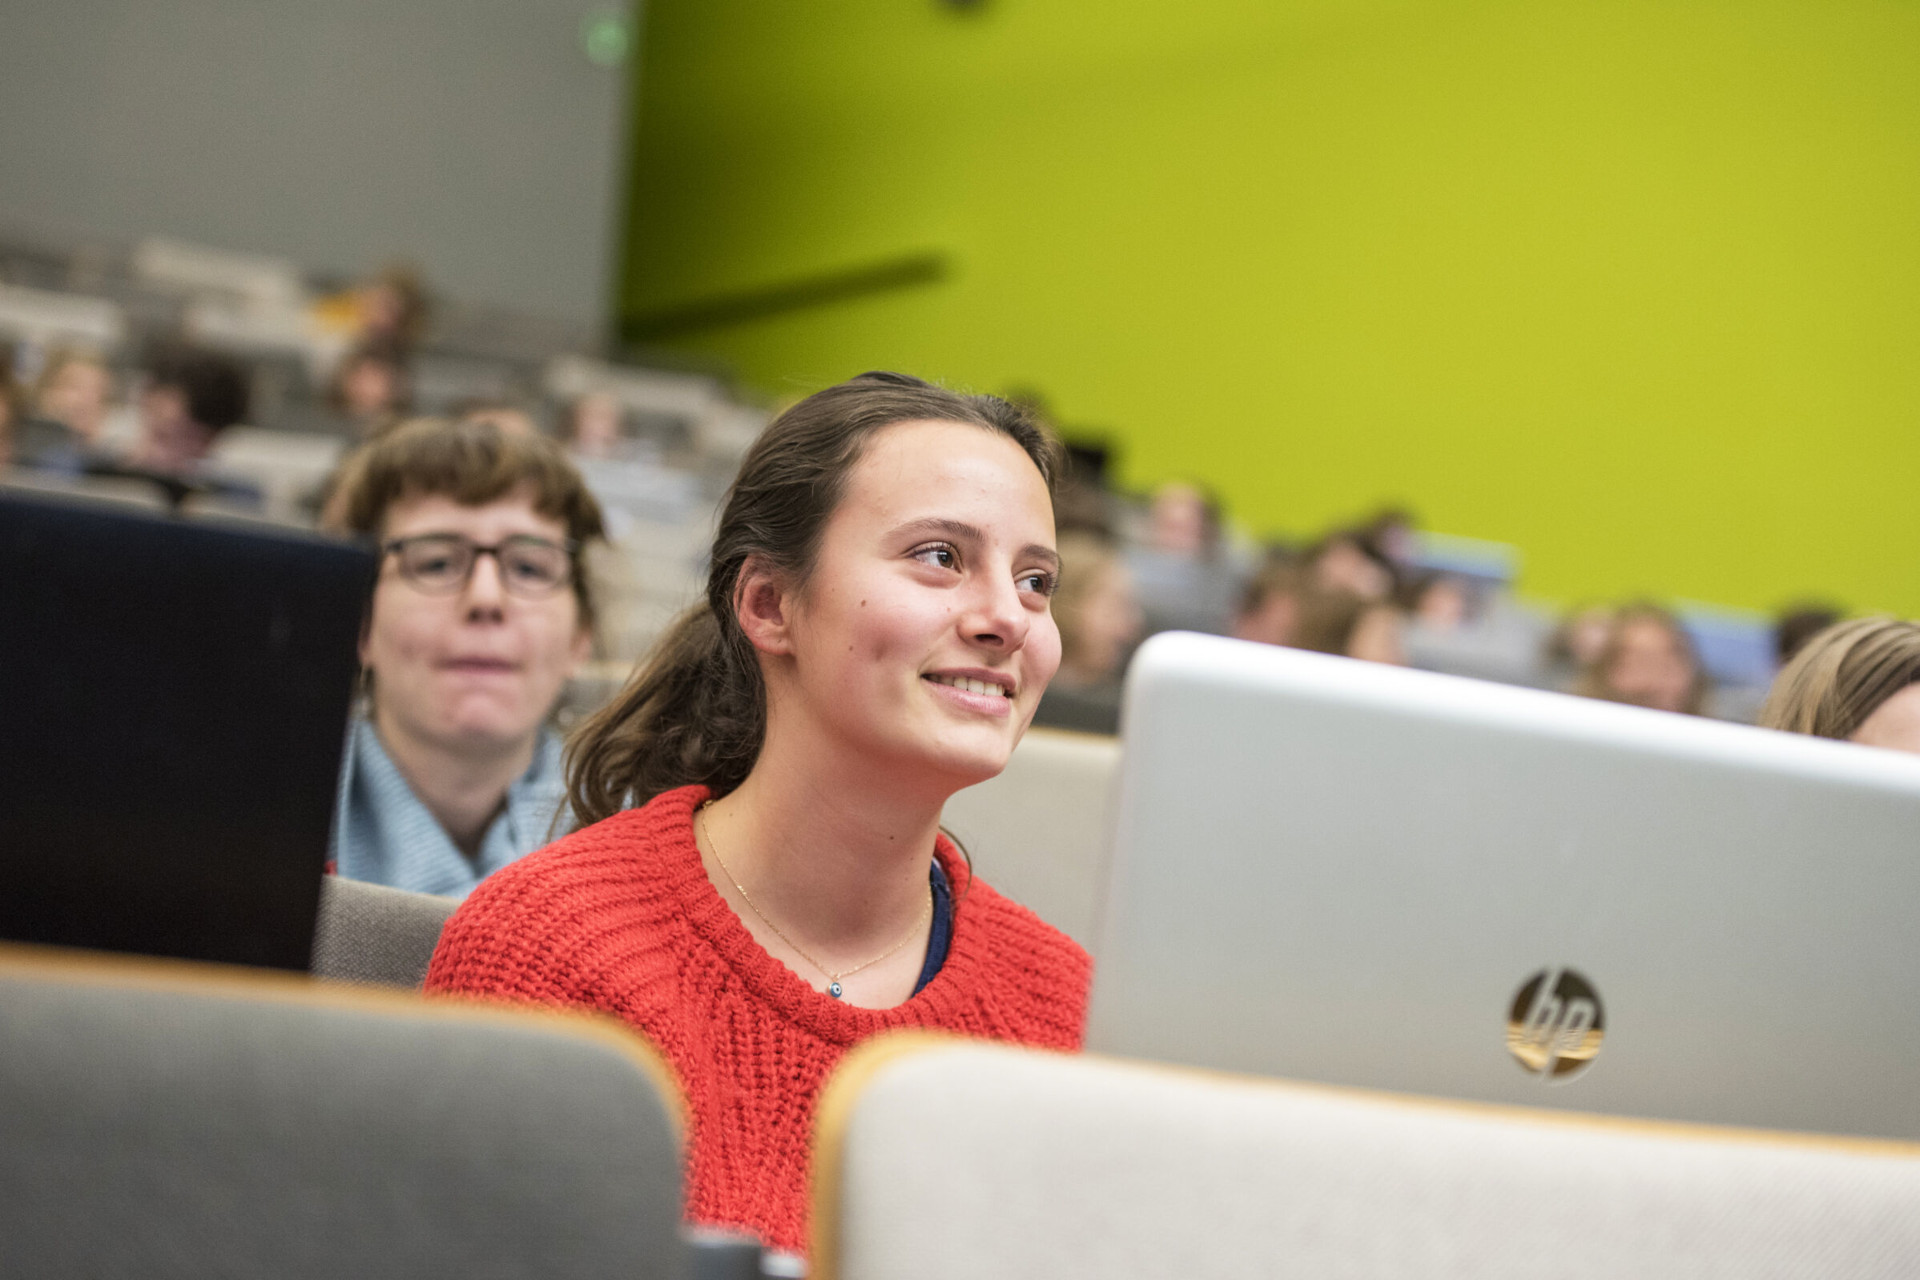
\includegraphics[scale=0.1,min width=0.5\paperwidth,min
    height=\textheight]{Images/uantwerpen-04.jpg}}]{
  \gdef\maybeinverse{}%
  \setbeamertemplate{background canvas}[lqgraphic]{#1}
  \@rqtexttrue
}

\define@key{beamerframe}{rhgraphic}
  [{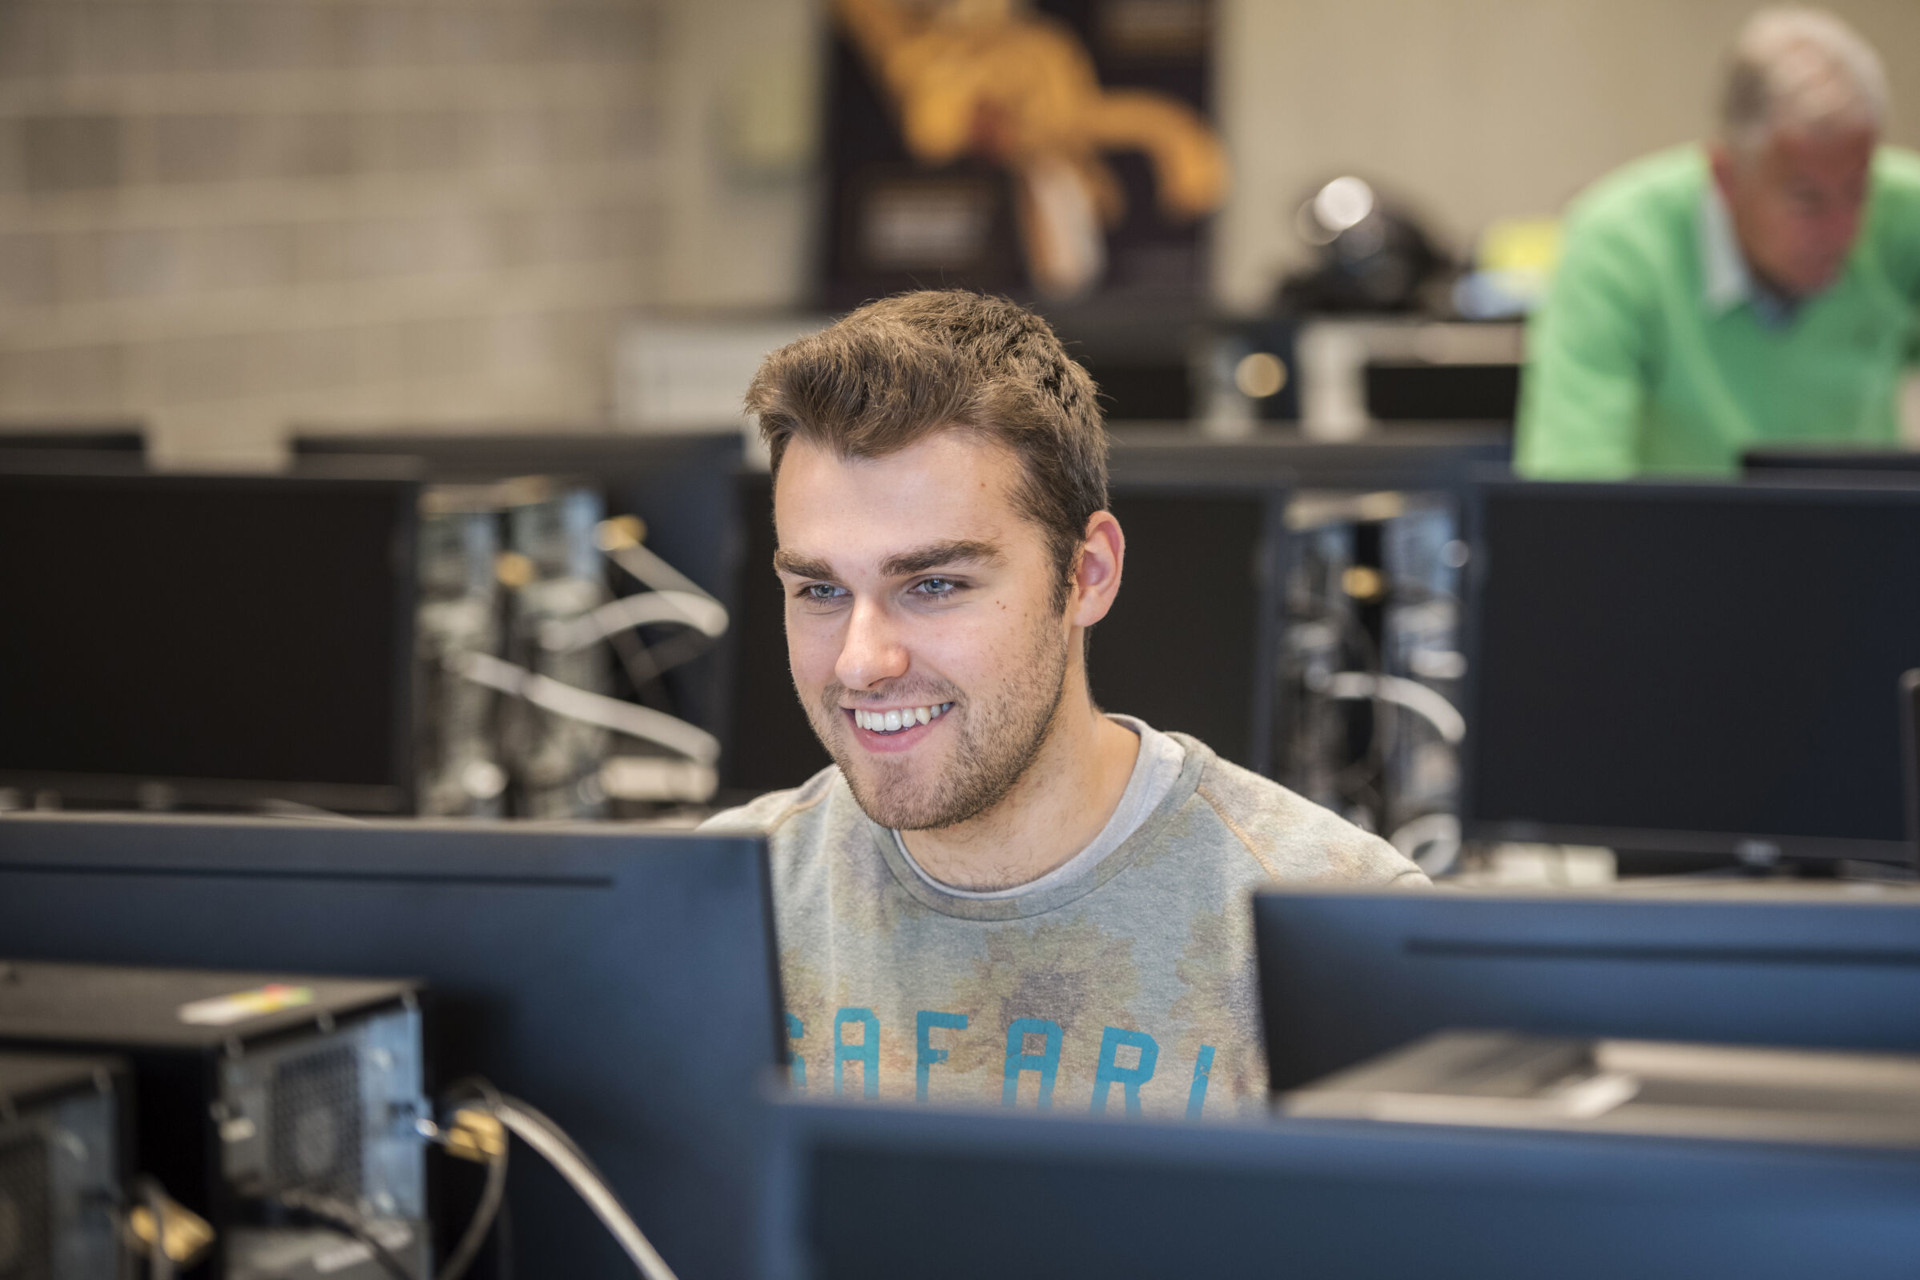
\includegraphics[scale=0.1,min width=0.5\paperwidth,min
    height=\textheight]{Images/uantwerpen-05.jpg}}]{ 
  \gdef\maybeinverse{}%
  \setbeamertemplate{background canvas}[rhgraphic]{#1}
  \@lhtexttrue
}

\define@key{beamerframe}{rqgraphic}
  [{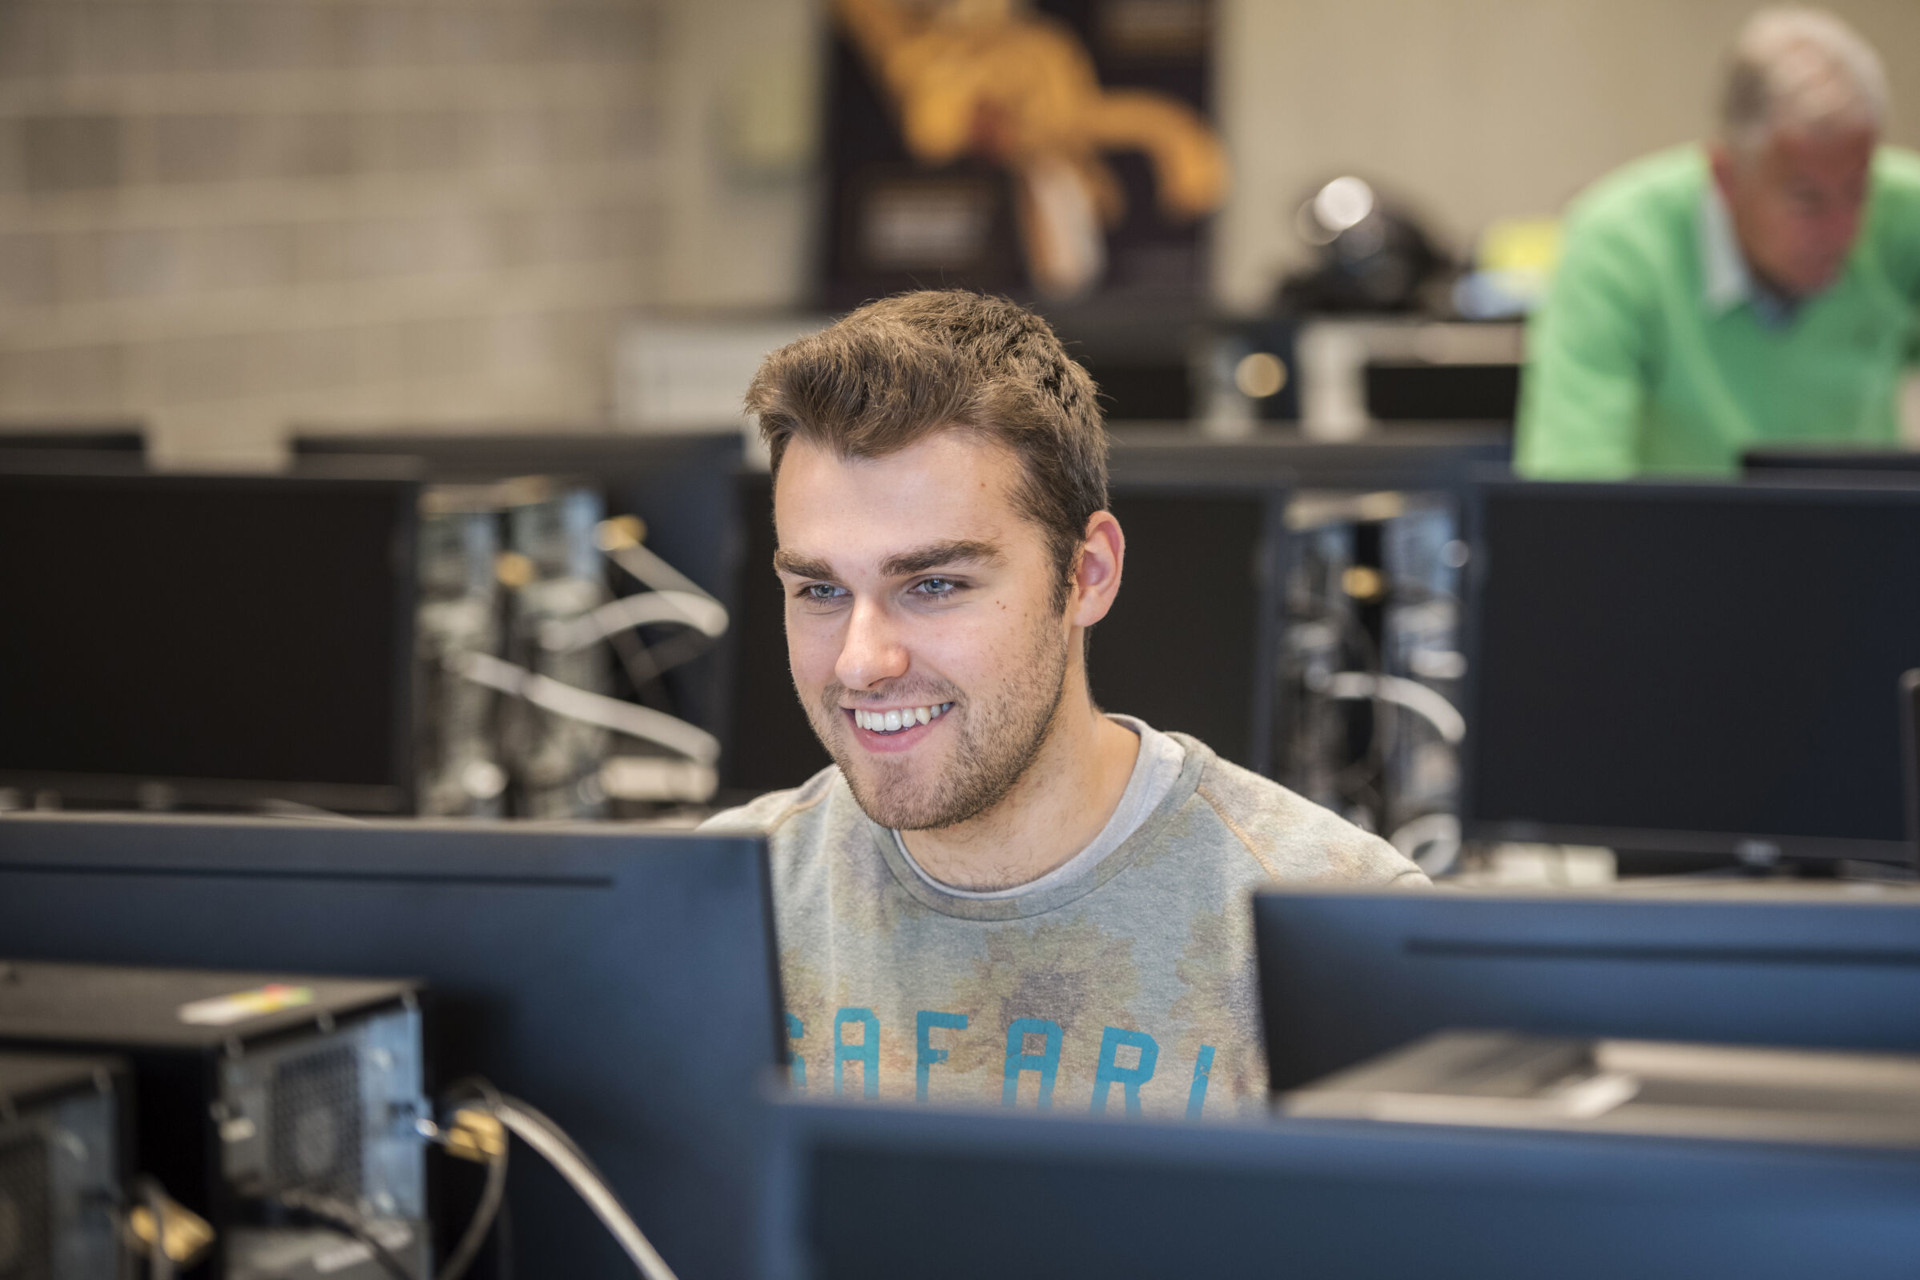
\includegraphics[scale=0.5,min width=0.5\paperwidth,min
    height=\textheight]{Images/uantwerpen-05.jpg}}]{ 
  \gdef\maybeinverse{}%
  \setbeamertemplate{background canvas}[rqgraphic]{#1}
  \@lqtexttrue
}

\define@key{beamerframe}{thgraphic}
  [{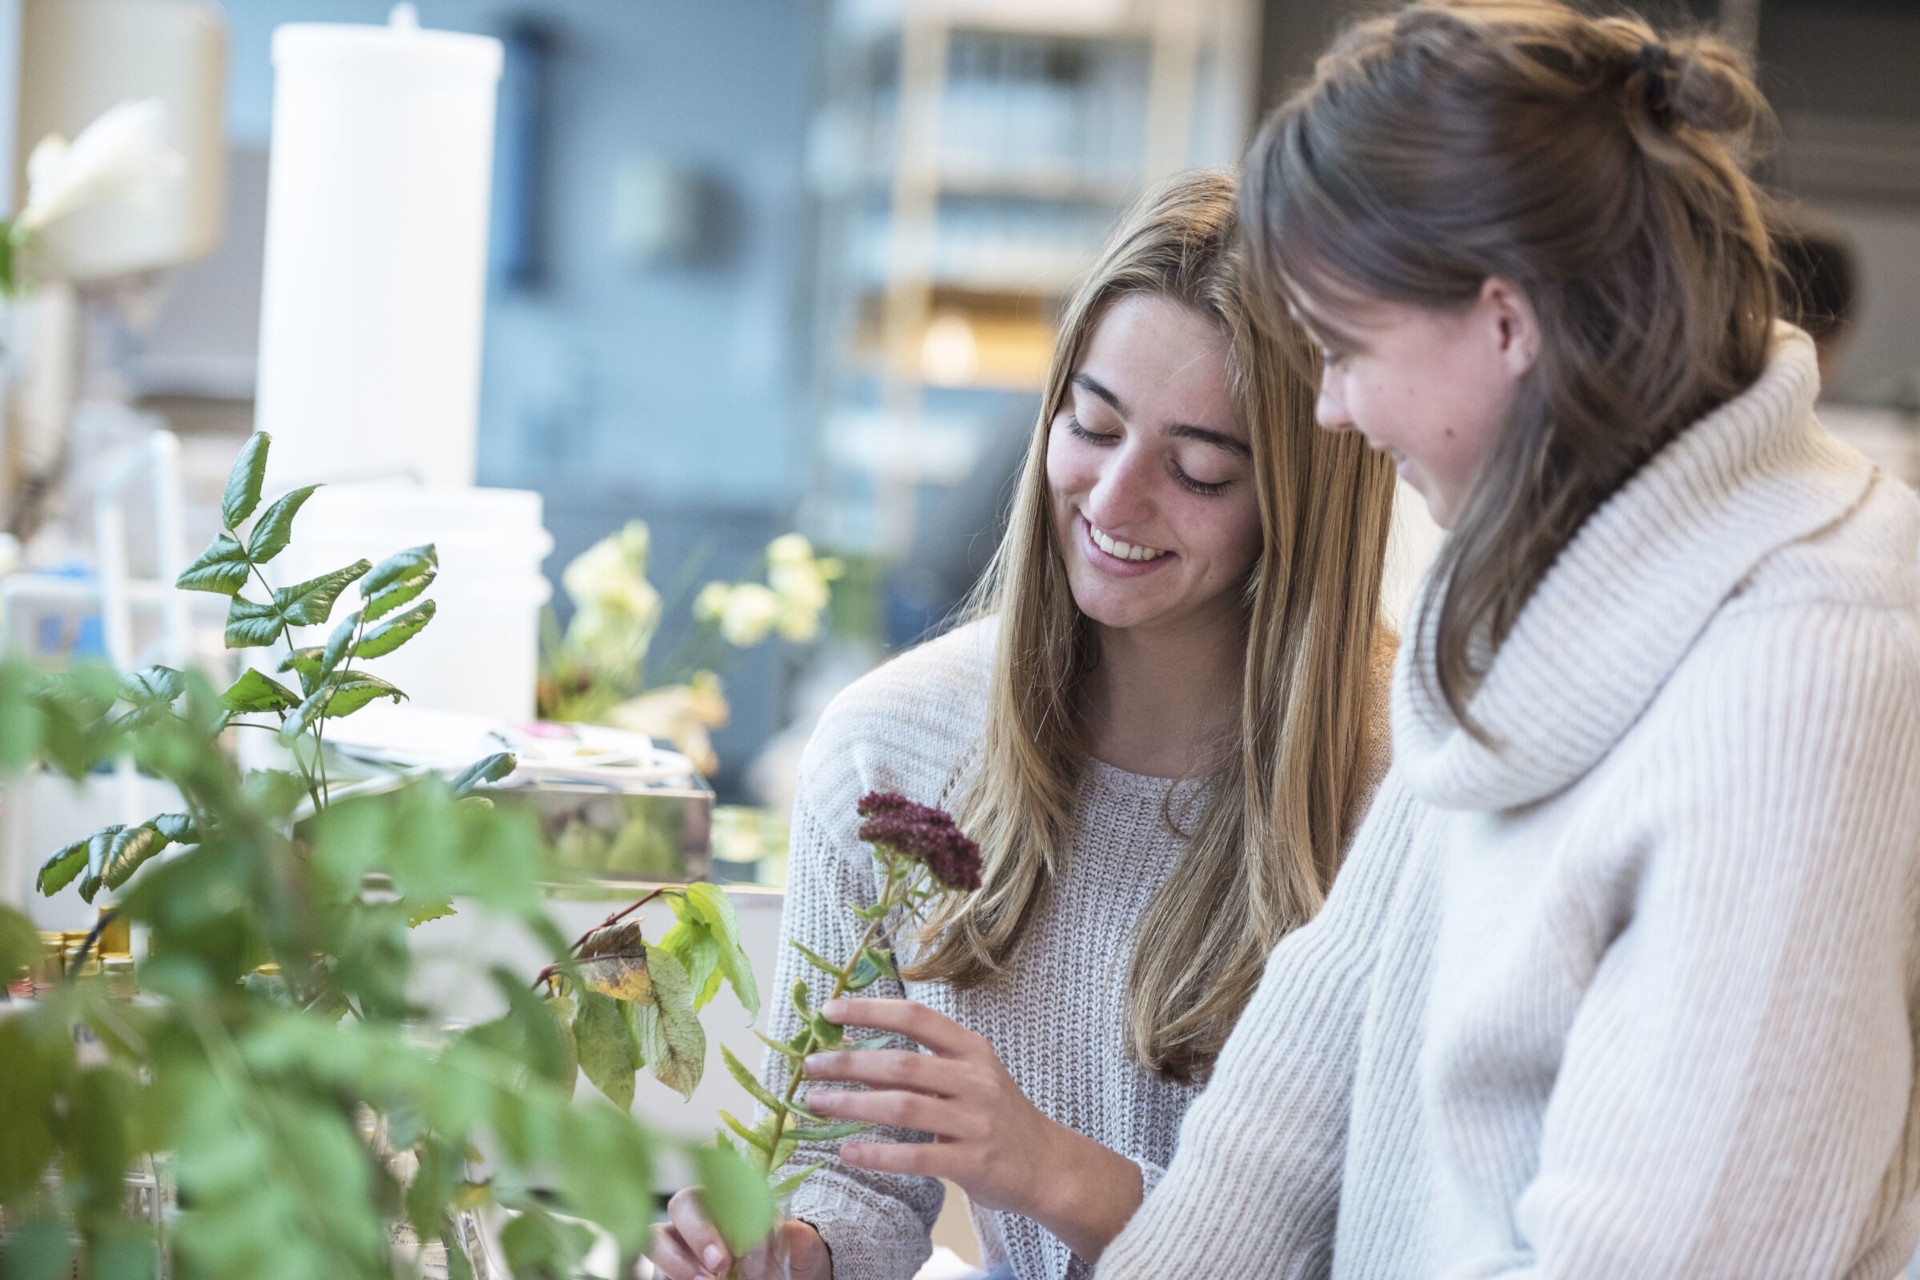
\includegraphics[scale=0.5,min width=\paperwidth,min
    height=0.5\textheight]{Images/uantwerpen-06.jpg}}]{ 
  \gdef\maybeinverse{}%
  \setbeamertemplate{background canvas}[thgraphic]{#1}
  \@bhtexttrue
}

\define@key{beamerframe}{bhgraphic}
  [{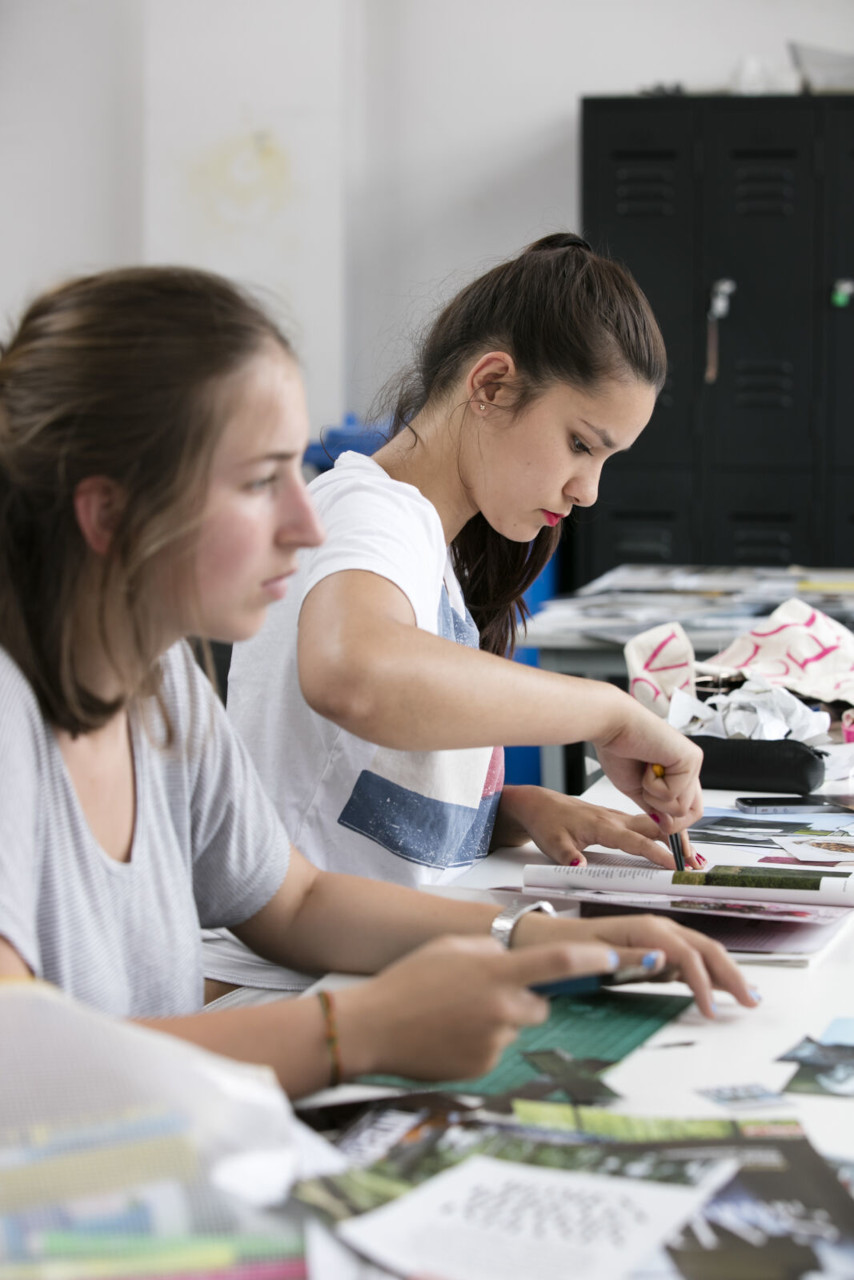
\includegraphics[scale=0.5,min width=\paperwidth,min
    height=0.5\textheight]{Images/uantwerpen-07.jpg}}]{ 
  \gdef\maybeinverse{}%
  \setbeamertemplate{background canvas}[bhgraphic]{#1}
}

\BeforeBeginEnvironment{frame}{%
  \gdef\maybeinverse{}%
  \setbeamertemplate{title page}[main]%
  \setbeamertemplate{section page}[main]%
  \setbeamertemplate{subsection page}[main]%
  \setbeamertemplate{background canvas}[normal]%
  \usebeamercolor[fg]{normal text}%
}

% The following does not work as \end{frame} is never executed by
% beamer!
% \AtEndEnvironment{frame}{\gdef\maybeinverse{}}

\NewEnviron{rhframe}[3][]{%
  \begin{frame}[#1]{#2}{#3}
    \begin{minipage}[t]{0.525\textwidth}
      ~
    \end{minipage}
    \begin{minipage}[t]{0.465\textwidth}
      \BODY
    \end{minipage}
  \end{frame}
}

\NewEnviron{r3qframe}[3][]{%
  \begin{frame}[#1]{#2}{#3}
    \begin{minipage}[t]{0.23\textwidth}
      ~
    \end{minipage}
    \begin{minipage}[t]{0.76\textwidth}
      \BODY
    \end{minipage}
  \end{frame}
}

\NewEnviron{lhframe}[3][]{%
  \begin{frame}[#1]{#2}{#3}
    \begin{minipage}[t]{0.465\textwidth}
      \BODY
    \end{minipage}
    \begin{minipage}[t]{0.525\textwidth}
      ~
    \end{minipage}
  \end{frame}
}

\NewEnviron{l3qframe}[3][]{%
  \begin{frame}[#1]{#2}{#3}
    \begin{minipage}[t]{0.77\textwidth}
      \BODY
    \end{minipage}
    \begin{minipage}[t]{0.22\textwidth}
      ~
    \end{minipage}
  \end{frame}
}

\NewEnviron{bhframe}[3][]{%
  \begin{frame}[#1]{#2}{#3}
      \BODY
  \end{frame}
}

\NewEnviron{thframe}[3][]{%
  \begin{frame}[#1]{#2}{#3}
      \BODY
  \end{frame}
}

%%%%%%%%%%%%
% Order:
% 1. option is executed
% 2. frametitle is typeset
% 3. canvas is typeset
% 4. frame is typeset
%%%%%%%%%%%%

\def\ps@uantwerpen@titlepage{%
  \setbeamercolor{title in title page}{parent=palette primary}
  \setbeamertemplate{footline}[empty]
  \@nameuse{ps@uantwerpen}
}

\defbeamertemplate*{background canvas}{negativefill}[1]
{%
  \gdef\appropriatelogo{\logomonowhite}%
  \gdef\appropriateslidenumber{\usebeamercolor{pageno in head/foot}%
    \insertframenumber/\inserttotalframenumber}%
  \color{maincolor}\vrule width\paperwidth height\paperheight
}

\defbeamertemplate*{background canvas}{negative}[1]
{%
  \gdef\appropriatelogo{\logopos}%
  \gdef\appropriateslidenumber{}%
  \begin{tikzpicture}
    \clip (0,0) rectangle (\pw,\ph);
    \uantwerpenleftshape[fill=maincolor]{(0.8,0.8)}{(\pw-0.8,\ph-0.8)}
  \end{tikzpicture}
}

\defbeamertemplate*{background canvas}{graphicfill}[1]
{%
  \gdef\appropriatelogo{\logoneg}%
  \gdef\appropriateslidenumber{}%
  \begin{tikzpicture}
    \clip (0,0) rectangle (\pw,\ph);
    \node[align=center] at  (0.5*\pw,0.5*\ph) {#1};
  \end{tikzpicture}%
}

\defbeamertemplate*{background canvas}{graphic}[1]
{%
  \gdef\appropriatelogo{\logopos}%
  \gdef\appropriateslidenumber{}%
  \begin{tikzpicture}
    \clip (0,0) rectangle (\pw,\ph);
    \begin{scope}
      \uantwerpenleftshape[clip]{(0.8,0.8)}{(\pw-0.8,\ph-0.8)}
      \node[align=center] at  (0.5*\pw,0.5*\ph) {#1};
    \end{scope}
  \end{tikzpicture}%
}

\defbeamertemplate*{background canvas}{lhgraphic}[1]
{%
  \gdef\maybeinverse{}%
  \gdef\appropriatelogo{\logopos}%
  \gdef\appropriateslidenumber{\usebeamercolor{pageno in head/foot}%
    \insertframenumber/\inserttotalframenumber}%
  \pgfmathsetmacro\dx{0.5*\pw-1.2}%
  \pgfmathsetmacro\dy{\ph-1.6}%
  \begin{tikzpicture}
    \clip (0,0) rectangle (\pw,\ph);
    \begin{scope}
      \uantwerpenleftshape[clip]{(0.8,0.8)}{(0.8+\dx,0.8+\dy)}
      \node[align=center] at  (0.8+0.5*\dx,0.8+0.5*\dy) {#1};
    \end{scope}
  \end{tikzpicture}
  \@tempswatrue
}

\defbeamertemplate*{background canvas}{lqgraphic}[1]
{%
  \gdef\maybeinverse{}%
  \gdef\appropriatelogo{\logopos}%
  \gdef\appropriateslidenumber{\usebeamercolor{pageno in head/foot}%
    \insertframenumber/\inserttotalframenumber}%
  \pgfmathsetmacro\dx{0.25*\pw-1.2}%
  \pgfmathsetmacro\dy{\ph-1.6}%
  \begin{tikzpicture}
    \clip (0,0) rectangle (\pw,\ph);
    \begin{scope}
      \uantwerpenleftshape[clip]{(0.8,0.8)}{(0.8+\dx,0.8+\dy)}
      \node[align=center] at  (0.8+0.5*\dx,0.8+0.5*\dy)
      {#1};
    \end{scope}
  \end{tikzpicture}
  \@tempswatrue
}

\defbeamertemplate*{background canvas}{rhgraphic}[1]
{%
  \gdef\maybeinverse{}%
  \gdef\appropriatelogo{\logopos}%
  \gdef\appropriateslidenumber{\usebeamercolor{pageno in head/foot}%
    \insertframenumber/\inserttotalframenumber}%
  \pgfmathsetmacro\dx{0.5*\pw-1.2}%
  \pgfmathsetmacro\dy{\ph-1.6}%
  \begin{tikzpicture}
    \clip (0,0) rectangle (\pw,\ph);
    \begin{scope}[shift={(0.5*\pw,0)}]
      \uantwerpenrightshape[clip]{(0.4,0.8)}{(0.4+\dx,0.8+\dy)}
      \node[align=center] at  (0.8+0.5*\dx,0.8+0.5*\dy) {#1};
    \end{scope}
  \end{tikzpicture}
  \@tempswatrue
}

\defbeamertemplate*{background canvas}{rqgraphic}[1]
{%
  \gdef\maybeinverse{}%
  \gdef\appropriatelogo{\logopos}%
  \gdef\appropriateslidenumber{\usebeamercolor{pageno in head/foot}%
    \insertframenumber/\inserttotalframenumber}%
  \pgfmathsetmacro\dx{0.25*\pw-1.2}%
  \pgfmathsetmacro\dy{\ph-1.6}%
  \begin{tikzpicture}
    \clip (0,0) rectangle (\pw,\ph);
    \begin{scope}[shift={(0.75*\pw,0)}]
      \uantwerpenrightshape[clip]{(0.4,0.8)}{(0.4+\dx,0.8+\dy)}
      \node[align=center] at  (0.8+0.5*\dx,0.8+0.5*\dy) {#1};
    \end{scope}
  \end{tikzpicture}
  \@tempswatrue
}

\defbeamertemplate*{background canvas}{thgraphic}[1]
{%
  \gdef\maybeinverse{}%
  \gdef\appropriatelogo{\logopos}%
  \gdef\appropriateslidenumber{\usebeamercolor{pageno in head/foot}%
    \insertframenumber/\inserttotalframenumber}%
  \pgfmathsetmacro\dx{\pw-1.6}%
  \pgfmathsetmacro\dy{0.5*\ph-0.8}%
  \begin{tikzpicture}
    \clip (0,0) rectangle (\pw,\ph);
    \begin{scope}[shift={(0,0.5*\ph)}]
      \uantwerpenleftshape[clip] {(0.8,0)}{(0.8+\dx,\dy)}
      \node[align=center] at  (0.8+0.5*\dx,0.5*\dy) {#1};
    \end{scope}
  \end{tikzpicture}
  \@tempswatrue
}

\defbeamertemplate*{background canvas}{bhgraphic}[1]
{%
  \gdef\maybeinverse{}%
  \gdef\appropriatelogo{\logopos}%
  \gdef\appropriateslidenumber{\usebeamercolor{pageno in head/foot}%
    \insertframenumber/\inserttotalframenumber}%
  \pgfmathsetmacro\dx{\pw-1.6}%
  \pgfmathsetmacro\dy{0.5*\ph-0.8}%
  \begin{tikzpicture}
    \clip (0,0) rectangle (\pw,\ph);
    \begin{scope}[shift={(0,0.8)}]
    \uantwerpenleftshape[clip] {(0.8,0)}{(0.8+\dx,\dy)}
    \node[align=center] at  (0.8+0.5*\dx,0.5*\dy) {#1};
    \end{scope}
  \end{tikzpicture}
  \@tempswatrue
}


\defbeamertemplate*{background canvas}{normal}
{%
  \gdef\maybeinverse{}%
  \gdef\appropriatelogo{\logopos}%
  \gdef\appropriateslidenumber{\usebeamercolor{pageno in
      head/foot}\insertframenumber/\inserttotalframenumber}%
}


\defbeamertemplate*{title page}{main}[1][]
{%
  \thispagestyle{uantwerpen@titlepage}%
  \begin{tikzpicture}
    \clip (0,0) rectangle (\textwidth,\paperheight-0.075cm);
    \node[anchor=center] at  (0.5*\textwidth,0.75*\ph)
    {\includegraphics[height=.9\logounitheight]{\logopos}};
    \node[
    text width=0.98\textwidth,
    text=basecolor,
    align=center] at (0.5*\textwidth,0.5*\ph) {
      \begin{beamercolorbox}[wd=\textwidth,center]{title in title page}
        \LARGE\bfseries\inserttitle\\[1ex]
        \usebeamercolor[fg]{subtitle in title page}
        \color{fg}\large\bfseries\insertsubtitle
      \end{beamercolorbox}
    };
    \node[
    text width=0.98\textwidth,
    color=basecolor,
    align=center] at (0.5*\textwidth,0.25*\ph) {
      \begin{beamercolorbox}[wd=\textwidth,center]{author in title page}
        \large\bfseries\insertauthor
      \end{beamercolorbox}
    };
    \node[
    text width=0.98\textwidth,
    color=basecolor,
    align=center] at (0.5*\textwidth,0.15*\ph) {
      \begin{beamercolorbox}[wd=\textwidth,center]{date in title page}
        \normalsize\bfseries\insertdate
      \end{beamercolorbox}
    };
  \end{tikzpicture}
}

\defbeamertemplate*{title page}{negative}[1][]
{
  \begin{tikzpicture}
    \clip (0,0) rectangle (\textwidth,\paperheight-0.075cm);
    \node[
    text width=0.98\textwidth,
    align=center] at (0.5*\textwidth,0.5*\ph) {
      \begin{beamercolorbox}[wd=\textwidth,center]{inverse title in title page}
        \LARGE\bfseries\inserttitle\\[1ex]
        \usebeamercolor[fg]{\maybeinverse subtitle in title page}
        \color{fg}\large\bfseries\insertsubtitle
      \end{beamercolorbox}
    };
    \node[
    text width=0.98\textwidth,
    align=center,] at (0.5*\textwidth,0.25*\ph) {
      \begin{beamercolorbox}[wd=\textwidth,center]{inverse author in title page}
        \large\bfseries\insertauthor
      \end{beamercolorbox}
    };
    \node[
    text width=0.98\textwidth,
    color=basecolor,
    align=center] at (0.5*\textwidth,0.15*\ph) {
      \begin{beamercolorbox}[wd=\textwidth,center]{inverse date in title page}
        \normalsize\bfseries\insertdate
      \end{beamercolorbox}
    };
  \end{tikzpicture}
}

\defbeamertemplate*{title page}{negativefill}[1][]
{
  \thispagestyle{uantwerpen@titlepage}
  \begin{tikzpicture}
    \clip (0,0) rectangle (\textwidth,\paperheight-0.075cm);
    \node[anchor=center] at  (0.5*\textwidth,0.75*\ph)
    {\includegraphics[height=.9\logounitheight]{\logomonowhite}};
    \node[
    draw,rectangle,
    text width=0.98\textwidth,
    color=maincolor,
    align=center] at (0.5*\textwidth,0.5*\ph) {
      \begin{beamercolorbox}[wd=\textwidth,center]{inverse title in title page}
        \LARGE\bfseries\inserttitle\\[1ex]
        \usebeamercolor[fg]{inverse subtitle in title page}
        \color{fg}\large\bfseries\insertsubtitle
      \end{beamercolorbox}
    };
    \node[
    text width=0.98\textwidth,
    color=maincolor,
    align=center] at (0.5*\textwidth,0.25*\ph) {
      \begin{beamercolorbox}[wd=\textwidth,center]{inverse author in title page}
        \large\bfseries\insertauthor
      \end{beamercolorbox}
    };
    \node[
    text width=0.98\textwidth,
    color=basecolor,
    align=center] at (0.5*\textwidth,0.15*\ph) {
      \begin{beamercolorbox}[wd=\textwidth,center]{inverse date in title page}
        \normalsize\bfseries\insertdate
      \end{beamercolorbox}
    };
  \end{tikzpicture}
}

\defbeamertemplate*{section page}{main}[1][]
{%
  \begin{tikzpicture}
    \clip (0,0) rectangle (\textwidth,\paperheight-0.075cm);
    \node[
    text width=0.98\textwidth,
    text=basecolor,
    align=center] at (0.5*\textwidth,0.55*\ph) {
      \begin{beamercolorbox}[wd=\textwidth,center]{section title}
        \Large\bfseries\insertsectionnumber.~\insertsection
      \end{beamercolorbox}
    };
  \end{tikzpicture}
}

\defbeamertemplate*{subsection page}{main}[1][]
{%
  \begin{tikzpicture}
    \clip (0,0) rectangle (\textwidth,\paperheight-0.075cm);
    \node[
    text width=0.98\textwidth,
    text=basecolor,
    align=center] at (0.5*\textwidth,0.55*\ph) {
      \begin{beamercolorbox}[wd=\textwidth,center]{section title}
        \Large\bfseries\insertsectionnumber.~\insertsection
      \end{beamercolorbox}
    };
    \node[
    text width=0.98\textwidth,
    text=basecolor,
    align=center] at (0.5*\textwidth,0.45*\ph) {
      \begin{beamercolorbox}[wd=\textwidth,center]{subsection title}
        \large\bfseries\insertsubsection
      \end{beamercolorbox}
    };
  \end{tikzpicture}
}

\defbeamertemplate*{section page}{negative}[1][]
{
  \begin{tikzpicture}
    \clip (0,0) rectangle (\textwidth,\paperheight-0.075cm);
    \node[
    text width=0.98\textwidth,
    text=basecolor,
    align=center] at (0.5*\textwidth,0.55*\ph) {
      \begin{beamercolorbox}[wd=\textwidth,center]{inverse section title}
        \Large\bfseries\insertsectionnumber.~\insertsection
      \end{beamercolorbox}
    };
  \end{tikzpicture}
}

\defbeamertemplate*{subsection page}{negative}[1][]
{
  \begin{tikzpicture}
    \clip (0,0) rectangle (\textwidth,\paperheight-0.075cm);
    \node[
    text width=0.98\textwidth,
    text=basecolor,
    align=center] at (0.5*\textwidth,0.55*\ph) {
      \begin{beamercolorbox}[wd=\textwidth,center]{inverse section title}
        \Large\bfseries\insertsectionnumber.~\insertsection
      \end{beamercolorbox}
    };
    \node[
    text width=0.98\textwidth,
    text=basecolor,
    align=center] at (0.5*\textwidth,0.45*\ph) {
      \begin{beamercolorbox}[wd=\textwidth,center]{inverse subsection title}
        \large\bfseries\insertsubsection
      \end{beamercolorbox}
    };
  \end{tikzpicture}
}

\defbeamertemplate*{footline}{empty}
{
}

\defbeamertemplate*{footline}{normal}
{%
  \leavevmode%
  \hbox{\begin{beamercolorbox}
      [wd=.5\paperwidth,ht=0.55cm,dp=0.25cm,left,leftskip=.8cm
      plus1fill]{author in head/foot}% 
      \includegraphics[height=0.35\logounitheight]{\appropriatelogo}
      \hskip0pt plus 1filll ~
  \end{beamercolorbox}%
  \begin{beamercolorbox}[wd=.5\paperwidth,ht=0.55cm,dp=0.25cm,
    right,rightskip=.8cm plus1fill]{\maybeinverse pageno in head/foot}%
    \usebeamerfont{pageno in head/foot}~\hskip0pt plus 1filll
    \appropriateslidenumber
  \end{beamercolorbox}}%
  \vskip0pt%
}

\defbeamertemplate*{frametitle}{empty}
{
}

\defbeamertemplate*{frametitle}{normal}
{%
  \vskip0.75cm%
  \if@rhtext%
  \@tempdima=0.5\textwidth%
  \@tempdimb=0.5\textwidth%
  \advance\@tempdima by0.5\beamer@leftmargin%
  \advance\@tempdimb by-0.5\beamer@leftmargin%
  \else%
  \if@rqtext%
  \@tempdima=0.23\textwidth%
  \@tempdimb=0.77\textwidth%
  \else%
  \if@lhtext%
  \@tempdima=0em%
  \@tempdimb=0.5\textwidth%
  \advance\@tempdimb by-0.5\beamer@leftmargin%
  \else%
  \if@lqtext%
  \@tempdima=0em%
  \@tempdimb=0.77\textwidth%
  \else%
  \if@bhtext%
  \@tempdima=0em%
  \@tempdimb=\textwidth%
  \vskip0.5\textheight%
  \else%
  \@tempdima=0em%
  \@tempdimb=\textwidth%
  \fi%
  \fi%
  \fi%
  \fi%
  \fi%
  \hskip\@tempdima%
  \begin{beamercolorbox}[wd=\@tempdimb]{\maybeinverse frametitle}%
    \usebeamerfont{frametitle}\insertframetitle\\[0.5ex]%
    \ifx\insertframesubtitle\@empty%
    {\usebeamerfont{framesubtitle}%
      \usebeamercolor[fg]{\maybeinverse framesubtitle}~\strut\par}%
    \vskip-1ex%
    \else%
    {\usebeamerfont{framesubtitle}%
      \usebeamercolor[fg]{\maybeinverse framesubtitle}%
      \insertframesubtitle\strut\par}%
    \fi%
    \if@tempswa\else\vskip-.3cm\fi% set inside beamercolorbox... evil here...
  \end{beamercolorbox}%
}

\newdimen\xloleft
\newdimen\yloleft
\newdimen\xupright
\newdimen\yupright
\newdimen\xcurrent
\newdimen\ycurrent
\newcommand*\extractloleftuadocs[1]{\path  (#1);\pgfgetlastxy{\xloleft}{\yloleft};}
\newcommand*\extractuprightuadocs[1]{\path (#1);\pgfgetlastxy{\xupright}{\yupright};}
\newcommand*\extractcurrentuadocs[1]{\path (#1);\pgfgetlastxy{\xcurrent}{\ycurrent};}

\DeclareRobustCommand\place{\@ifnextchar[{\@place}{\@place[align=left] }}
\def\@place[#1] at (#2,#3)#4{
  \begin{tikzpicture}[overlay,remember picture]
    \extractloleftuadocs{$(current page.south west)$}
    \extractuprightuadocs{$(current page.north east)$}
    \node[#1] at
    ({\xloleft*(1-#2)+\xupright*#2},{\yloleft*(1-#3)+\yupright*#3}) {#4};
  \end{tikzpicture}
}

\mode
<all>
%</bmrouter>
%    \end{macrocode}
%
% \Finale
\endinput
